\chapter{Analysis of High Mass Drell-Yan Transverse Spin Phenomena}
\label{ch::hmanalysis}
\ifpdf
\graphicspath{{Chapters/HMAnalysis/Figs/}}
\fi

This chapter goes over the analysis techniques and results from the 2015
transversely polarized Drell-Yan data taking.  The chapter begins by describing
the data collection setup and the event selection criteria followed by the
analysis techniques used to determine asymmetry amplitudes.  The analysis
techniques described are: the standard transverse spin-dependent asymmetry (TSA)
analysis, Sec~\ref{sec::standTSA}, the double ratio analysis,
Sec~\ref{sec::doubleratio}, the $q_T$ weighted asymmetry analysis,
Sec~\ref{sec::qtweighted}, and finally the left-right asymmetry analysis,
Sec~\ref{sec::leftrightasym}.  All of these analyses are related in that they
measure TMD effects from the Drell-Yan process.  For this reason the event
selection and kinematical asymmetry binning described in the opening sections
will be the same for all analyses in this chapter unless stated otherwise.

\section{Data Sample} \label{sec::datasample}

\subsection{Data Collection} \label{sec::datacollection}

The data sample is from the 2015 COMPASS Drell-Yan measurement.  In this
measurement a 190~GeV/c $\pi^-$ beam impinged on a transversely polarized NH$_3$
target and two oppositely charged muons were detected in the spectrometer.
Fig.~\ref{fig::dy_2015_targ_setup} gives a visual of the basic setup and
chapter~\ref{ch::compass} goes over the spectrometer setup and beam in more
details.  The COMPASS spectrometer began taking commissioning data in April of
2015.  The data collected for this analysis, after the commissioning phase, is
from July 8 through November 12 of 2015.  After November 12, the SPS stopped
providing beam for a winter shut down.  The data is split into 9 periods lasting
approximated 2 weeks each and labeled W07-W15.  During each data period the
spectrometer conditions were frozen so no detector changes could affect the
spectrometer acceptance.  Sec~\ref{sec::polTarget} describes the polarized
target in more details.  In summaray, the NH$_3$ target was split into two
oppositely polarized cells separated by 20~cm with one cell polarized vertically
up and one cell polarized vertically down in the lab frame.  Each data period is
split into two sub-periods to reduce systematic effects of acceptance and
luminosity dependencies.  The polarization of both cells was flipped between
sub-periods.  A summary of the analysis data taking from each period is shown in
Table~\ref{tab::datataking}.

\begin{figure}[h!t]
  \centering 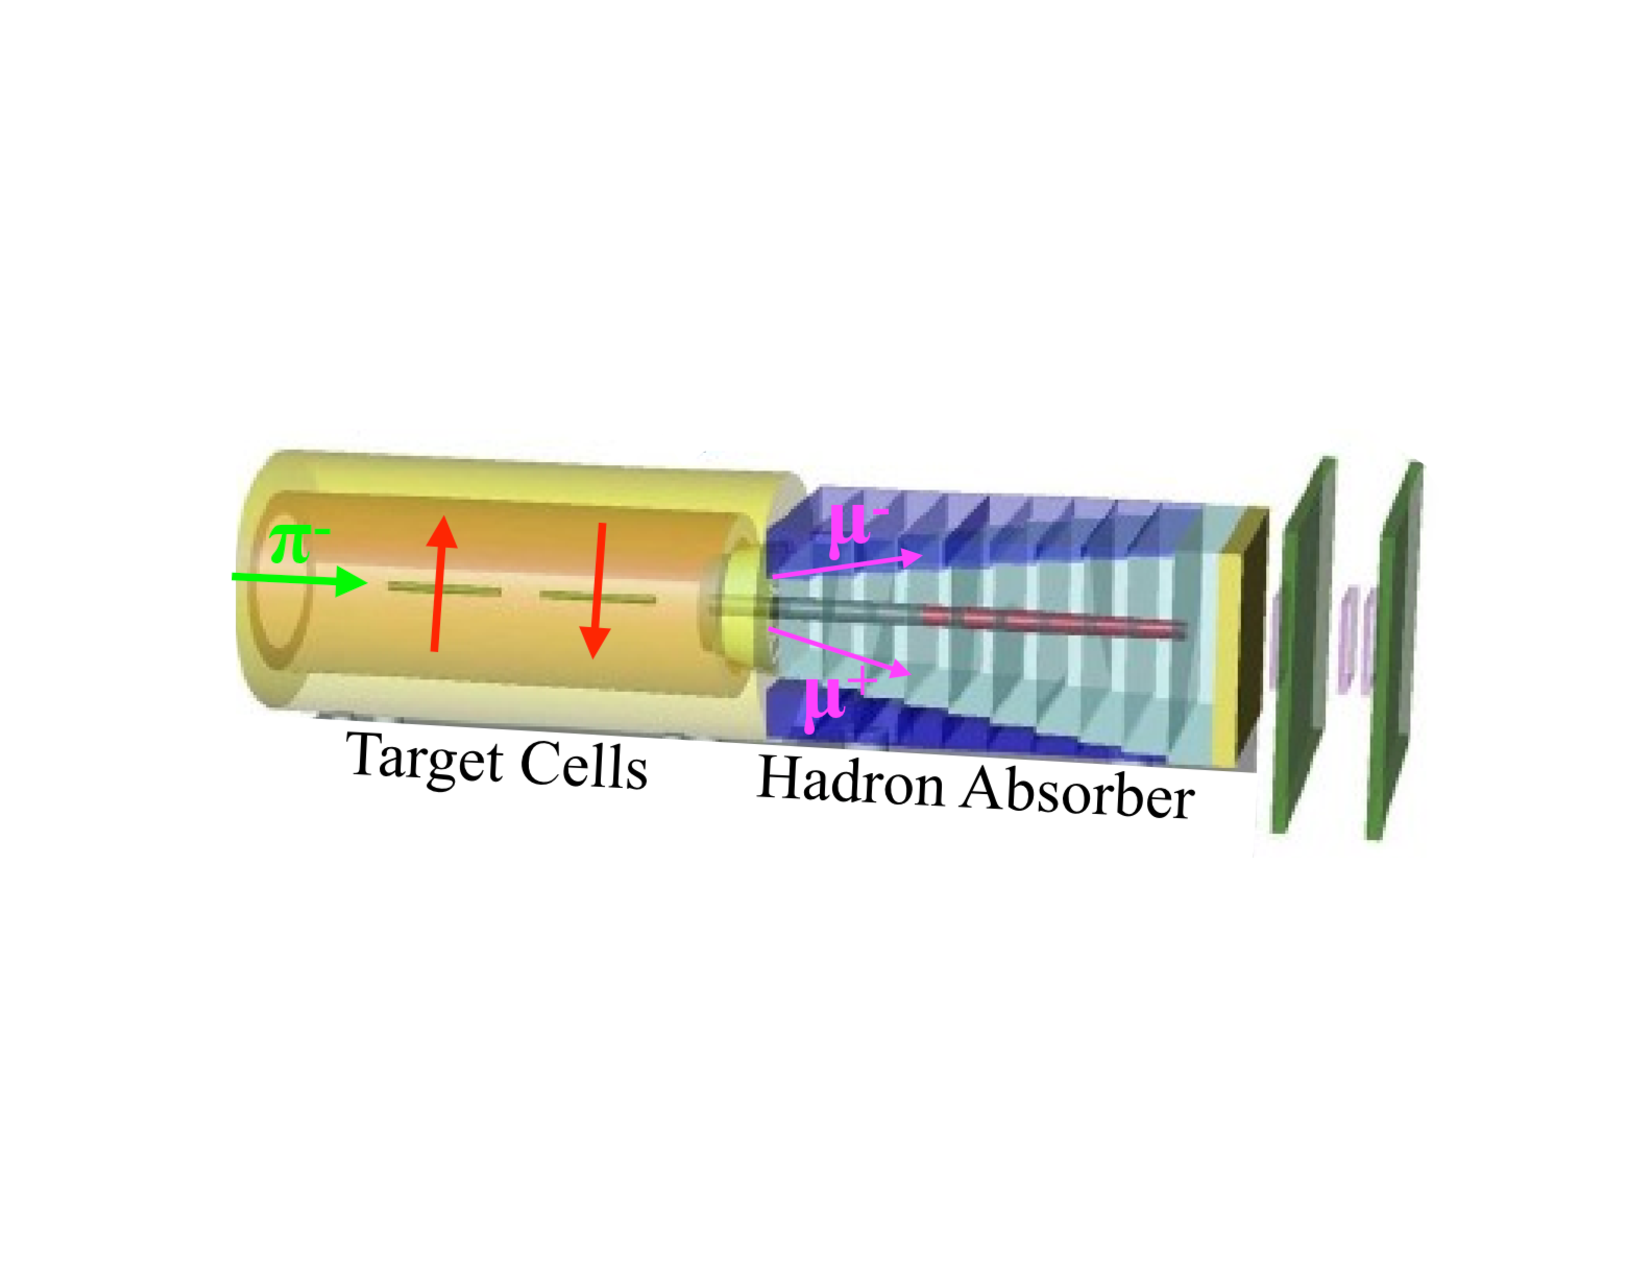
\includegraphics[width=0.6\textwidth, trim=4cm 7cm 4cm 7cm,
    clip]{dy_2015_targ_setup}
  \caption{Basic pictorial setup of the target region in 2015 COMPASS Drell-Yan
    data collection.}
  \label{fig::dy_2015_targ_setup}
\end{figure}


\begin{table}[h!t]
  \centering
  \begin{tabular}{ |c|c|c|c|c|c| }
    \hline Period& Sub-period& Polarization& First-Last run& Begin date& End
    date \\ \hline
    
    \multirow{2}{2em}{W07}& one& $\downarrow \uparrow$& 259363 - 259677& July
    9& July 15 \\ & two& $\uparrow \downarrow$& 259744 - 260016& July 16& July
    22 \\ \hline

    \multirow{2}{2em}{W08}& one& $\uparrow \downarrow$& 260074 - 260264& July
    23& July 29 \\ & two& $\downarrow \uparrow$& 260317 - 260565& July 29&
    August 5 \\ \hline

    \multirow{2}{2em}{W09}& one& $\downarrow \uparrow$& 260627 - 260852&
    August 5& August 12 \\ & two& $\uparrow \downarrow$& 260895 - 261496&
    August 12& August 26 \\ \hline

    \multirow{2}{2em}{W10}& one& $\uparrow \downarrow$& 261515 - 261761&
    August 26& September 1 \\ & two& $\downarrow \uparrow$& 261970 - 262221&
    September 4& September 9 \\ \hline

    \multirow{2}{2em}{W11}& one& $\downarrow \uparrow$& 262370 - 262772&
    September 11& September 22 \\ & two& $\uparrow \downarrow$& 262831 -
    263090& September 23& September 30 \\ \hline

    \multirow{2}{2em}{W12}& one& $\uparrow \downarrow$& 263143 - 263347&
    September 30& October 7 \\ & two& $\downarrow \uparrow$& 263386 - 263603&
    October 8& October 14 \\ \hline

    \multirow{2}{2em}{W13}& one& $\downarrow \uparrow$& 263655 - 263853&
    October 15& October 21 \\ & two& $\uparrow \downarrow$& 263926 - 264134&
    October 22& October 28 \\ \hline

    \multirow{2}{2em}{W14}& one& $\uparrow \downarrow$& 264170 - 264330&
    October 28& November 2 \\ & two& $\downarrow \uparrow$& 264429 - 264562&
    November 4& November 8 \\ \hline

    \multirow{2}{2em}{W15}& one& $\downarrow \uparrow$& 264619 - 264672&
    November 9& November 11 \\ & two& $\uparrow \downarrow$& 264736 - 264857&
    November 12& November 16 \\ \hline
    
  \end{tabular}
  \caption{COMPASS 2015 data taking periods}
  \label{tab::datataking}
\end{table}

\subsection{Stability Tests} \label{sec::stability}
To ensure the data analyzed were recorded during stable beam and spectrometer
conditions, stability of the analysis data was performed on a spill-by-spill and
run-by-run basis.  The data was recorded in runs with a maximum of 200 spills
per run.  One spill can have several thousand events.

\subsubsection{Bad Spill Analysis} To determine if a given spill is deemed
unstable several macro variables were averaged over per spill and compared to
neighboring spill averages.  These macro variables were chosen specifically to
be sensitive to the general stability conditions of the data collection and are
listed in the following itemized list.  The analysis criteria for an bad
spill events was two oppositely charged muons.  A muon is defined as having
crossed 15 radiation lengths of material.

\begin{itemize}
\item number of beam particles divided by the number of events
\item number of beam particles divided by the number of primary vertices
\item number of hits per beam track divided by the number of beam particles
\item number of primary vertices divided by the number of events
\item number of outgoing tracks divided by the number of events
\item number of outgoing particles from a primary vertex divided by the number
  of primary vertices
\item number of outgoing particle from primary vertex divided by the number of
  events
\item number of outgoing particles from primary vertex divided by the number of
  events
\item number of hits from outgoing particles divided by the number outgoing
  particles
\item number of $\mu^+$ tracks divided by the number of events
\item number of $\mu^+$ tracks from primary vertex divided by the number of
  events
\item number of $\mu^-$ tracks divided by the number of events
\item number of $\mu^-$ tracks from primary vertex divided by the number of
  events
\item $\sum \chi^2$ of outgoing particles divided by the number of outgoing
  particles
\item $\sum \chi^2$ of all vertices divided by the number of all vertices in an
  event
\item Trigger rates (LASxLAS, OTxLAS, LASxMT)
\end{itemize}

If the data collected was stable during a spill the average values from the
macro variables in the above itemized list are expected to be constant
from one spill to the next.  To determine if a spill was recorded in unstable
conditions the spill of interest is compared with its neighboring 2500 spills
occurring before and after in time.  If the spill of interest is over a
specified sigma deviation from any of the neighboring spills too many times, the
spill is mark as a bad spill.  If a spill fails this bad spill criteria for any
of the macro variables in the above itemized list, the spill is deemed
bad and not included in the analysis.  The criteria for the sigma distance and
number of times a spill crosses this distance to be deemed a bad are different
for each data taking period.  In addition to checking the nearest neighbor
spills, an entire run is marked bad if the run has less than 10 spills or
greater than 70\% bad spills.  Table~\ref{tab::badspillpercent} describes the
bad spill impact on each period. \par

\subsubsection{Bad Run Analysis}
The stability of the spectrometer is also verified by a run-by-run check in
parallel to the spill-by-spill checks.  The run-by-run analysis compares
kinematic distributions and the average of these distributions per run to the
kinematic distributions and averages from the other runs in a given period.  The
distributions tested are: x$_{\mathrm{N}}$, x$_{\pi}$, x$_{\mathrm{F}}$,
q$_{\mathrm{T}}$, M$_{\mu\mu}$, P$_{\mu^+}$, P$_{\mu^-}$, P$_{\gamma}$,
P$_{\pi^-}$, and vertex x, y and z positions.  The quantities in the run-by-run
analysis are expected to influence the asymmetries measured, however their
distributions and averages are not expected to have spin-influenced effects from
the limited statistics in just a single run.

The distributions are compared with an unbinned-Kolmogorov test and the
averages over a distribution are compared based on their deviations from each
other.  The unbinned-Kolmogorov test is made between all the runs in a given
period.  A run is marked bad if it is incompatible with most of the runs in a
period.  Additionally, the mean for each distribution in a run is is compared
with the average from a given period.  When an average kinematical variables
from a run is more than five standard deviations from the average within a
period, the run is rejected.  The results of the bad spill rejection after
having already applied the bad spill rejection are shown in
Table~\ref{tab::badspillpercent}.

\begin{table}[h!t]
  \centering
  \begin{tabular}{ |c|c|c| }
    \hline \textbf{Period}& \textbf{Bad Spill Rejection}&
    \textbf{Bad Spill and Bad Run Rejection} \\ \hline \hline
    
    W07& 11.79\%& 17.94\%\\ \hline
    W08& 18.00\%& 21.19\%\\ \hline
    W09& 14.76\%& 17.11\%\\ \hline
    W10& 15.88\%& 17.80\%\\ \hline
    W11& 22.49\%& 26.14\%\\ \hline
    W12& 12.71\%& 13.79\%\\ \hline
    W13& 22.32\%& 22.73\%\\ \hline
    W14& 8.91\%& 10.70\%\\ \hline
    W15& 3.94\%& 3.94\%\\ \hline

  \end{tabular}
  \caption{Stability analysis rejection percentages}
  \label{tab::badspillpercent}
\end{table}

\subsection{Event Selection} \label{sec::dy_eventselection}
The cuts in the event selection were chosen to ensure the event consisted of two
oppositely charged muons resulting from a pion collision in the transversely
polarized target.  The event selection was initial filtered from miniDSTs to
$\mu$DSTs where only events with at least two muons detected were kept in the
$\mu$DSTs.  The cuts used in this analysis are described in the following
enumerated list, where the event selection is performed on the $\mu$DSTs and the
events used are from the slot1 reconstruction.  A summary of the number of
events remaining after the last cuts is shown in Table~\ref{tab::EventTable}.

\begin{enumerate}
\item Two oppositely charged particles from a common best primary vertex having
  an invariant mass between 4.3~{\gvcw} and 8.5~{\gvcw}.  A primary vertex is
  defined as any vertex with an associated beam particle.  In case of multiple
  common primary vertices the best primary vertex is determined by CORAL tagging
  the vertex as best primary (PHAST method PaVertex::IsBestPrimary()).  In the
  case that CORAL did not tag any of the common vertices as the best primary the
  vertex with the smallest spatial $\chi^2$ value is used as the best primary
  vertex.  The mass range of 4.3~{\gvcw} through 8.5~{\gvcw} is deemed the high
  mass range.  Fig.~\ref{fig::DY_InvariantMass} shows the mass invariant mass
  distribution and the background components.  The mass range between 4.3 and
  8.5~{\gvcw} corresponds to over 96~\% Drell-Yan events.
\item A dimuon trigger fired.  A dimuon trigger firing means there are at least
  two particles in coincidence in this event. The dimuon triggers used were a
  coincidence between two particles in the large angle spectrometer, LAS-LAS
  trigger, or a particle in the large angle spectrometer and a particle in the
  Outer hodoscope, LAS-Outer trigger.  The triggering process is further
  described in Sec~\ref{sec::trigger}.  The LAS-Middle trigger was used as a
  veto on beam decay muons.  A beam decay muon results from the decay of a beam
  pion, kaon or anti-proton into a muon depicted as $\pi^- \rightarrow \mu^- +
  \bar{\nu}_{\mu^-}$, $K^- \rightarrow \mu^- + \bar{\nu}_{\mu^-}$, or $\bar{p}
  \rightarrow \mu^- + \bar{\nu}_{\mu^-}$ respectively.  A beam decay muon can
  then be in coincidence with a positive muon from another decay or strong
  reaction in the target resulting in an unwanted background process.  The
  LAS-Middle trigger was used as a veto because this trigger was found to have
  many events resulting from a beam pion decaying to a muon.
\item Both particles are muons.  A muon was defined as having crossed 30
  radiation lengths of material between the particles first and last measured
  points.  This criteria has been previously been determined to be effective at
  distinguishing between muons and hadrons.  In the data production no
  detectors were used from upstream of the hadron absorber so the absorber is
  not included in the determination of material crossed.
\item The first measured point for both particles occurs before 300~cm and the
  last measured point occurs after 1500~cm.  This cut ensures both particles
  have positions upstream of the first spectrometer magnet and downstream of the
  first muon filter.
\item The timing of both muons is defined.  This checks that the time relative
  to the trigger time is determined for both muons so further timing cuts can be
  performed.
\item Both muons are in time within 5~nanoseconds.  This track time for each
  muon is defined relative to the trigger time as in the previous cut.  This cut
  rejects uncorrelated muons.
\item The muon track's spacial reduced $\chi^2$ are individually less than 10.
  This cut ensures track quality.
\item A validation that each muon crossed the trigger it was associated as
  having triggered.  This trigger validation cut was performed by extrapolating
  (PHAST Method PaTrack::Extrapolate()) each muon track back to the two
  hodoscopes it fired and determining if the muon crossed the geometric
  acceptance of both of these hodoscopes.
\item The event does not occur in the bad spill or run list.  Many tests were
  performed to test the basic stability of the spectrometer and beam as
  described in Sec~\ref{sec::stability}.  The spills placed on the bad spill
  list were deemed to occur during unstable data taking conditions.
\item The Drell-Yan kinematics are physical.  That is $0 < x_{\pi} \;
  x_{\mathrm{N}} < 1$ and $-1 < x_{\mathrm{F}} < 1$.
\item The transverse momentum of the virtual photon, $q_T$, is between 0.4 and
  5.0 GeV/c.  The lower limit ensures the azimuthal angular resolution is
  sufficient and the upper cut further ensures the kinematic distributions are
  physically possible and not badly reconstructed events.
\item The vertex originated within the z-positions of the transversely polarized
  target cells defined by the target group.  -294.5~cm$<$ Z$_{\mathrm{vertex}}$
  $<$-239.3~cm for the upstream target and -219.5~cm$<$ Z$_{\mathrm{vertex}}$
  $<$-164.3~cm for the downstream target.
\item The vertex is within the radius of the polarized target measured to be
  1.9~cm.
\end{enumerate}

\begin{table}[h!t]
  \begin{adjustwidth}{-2cm}{}
    \begin{tabular}{ |c|c|c|c|c|c|c|c|c|c|c|c| }
      \hline \textbf{Cuts}& \textbf{W07}& \textbf{W08}& \textbf{W09}&
      \textbf{W10}& \textbf{W11}& \textbf{W12}& \textbf{W13}& \textbf{W14}&
      \textbf{W15} & \textbf{WAll} & \textbf{Remaining} \\ \hline

      \multirow{2}{13em}{High Mass $\mu^-\mu^+$ with a common best primary
        vertex}& 19410& 19184& 19654& 20707& 31371& 23563& 20561& 13154& 7697&
      175301& 100.00 \% \\ & & & & & & & & & & & \\ \hline
      
      Good Spills& 15947& 14899& 16217& 16895& 23041& 20184& 16026& 11796& 7422&
      142427& 81.70 \% \\ \hline

      0$<$ x$_{\pi}$ x$_N$ $<$1, -1$<$ x$_F$ $<$1& 15932& 14886& 16200& 16885&
      23022& 20171& 16013& 11794& 7414& 142317& 81.70 \% \\ \hline

      0.4$<$ q$_T$ $<$5(GeV/c)& 14342& 13385& 14609& 15239& 20667& 18101& 14365&
      10588& 6636& 127932& 60.75 \% \\ \hline

      Z Vertex within NH$_3$& 4256& 4024& 4330& 4552& 6369& 5503& 4411& 3130&
      2028& 38603& 15.05 \% \\ \hline

      Vertex Radius $<$ 1.9cm& 4175& 3950& 4257& 4474& 6252& 5414& 4334& 3078&
      1987& 37921& 12.21 \% \\ \hline
      
    \end{tabular}
    \caption{Numbers of selected di-muon events in this analysis of 2015 COMPASS
      data}
    \label{tab::EventTable}
  \end{adjustwidth}
\end{table}

\subsection{Binning}
The asymmetries are measured in bins of $x_N$, $x_{\pi}$, $x_F$,
$q_T$, and $M_{\mu\mu}$. $x_N$ and $x_{\pi}$ are the momentum
fractions of the target nucleon and beam pion respectively, $x_F$ =
$x_{\pi} - x_N$, $q_T$ is the transverse momentum of the virtual
photon and $M_{\mu\mu}$ is the invariant mass of the di-muon.  The binning was
determined by requiring equal statistical population in each kinematic bin.  In
addition, the asymmetries are determined in an integrated bin using all the
analysis data.  The analyzes binning limits are summarized in
Table~\ref{tab::binning}.

\begin{table}[h!t]
  \centering
  \begin{tabular}{ |c|c|c|c|c| }
    \hline \textbf{Kinematics}& \textbf{Lowest limit}& \textbf{Upper limit bin
      1}& \textbf{Upper limit bin 2}& \textbf{Upper limit bin 3}\\ \hline
    
    $x_N$& 0.0& 0.13& 0.19& 1.0\\ \hline $x_{\pi}$& 0.0& 0.40& 0.56&
    1.0\\ \hline $x_F$& -1.0& 0.22& 0.41& 1.0\\ \hline $q_T$ (GeV/c)& 0.4& 0.86&
    1.36& 5.0\\ \hline $M_{\mu\mu}$ (GeV/c$^2$)& 4.3& 4.73& 5.50& 8.5 \\ \hline
    
  \end{tabular}
  \caption{Analysis binning limits}
  \label{tab::binning}
\end{table}

\subsection{Analysis Notation}
Table~\ref{tab::ANnotations} summarizes the general notations used in the
asymmetry analysis definitions and derivations used throughout this chapter.

\begin{table}[h!t]
  \centering
  \caption{Notations used for defining the asymmetry analysis}
  \label{tab::ANnotations}
  \begin{tabular}{ |c|c| }
    
    \hline \textbf{Notation}& \textbf{Description}
    \\ \hline 1(2)& target cell
    number. 1=upstream, 2=downstream \\ \hline
    $\uparrow(\downarrow)$ & target
    cell vertical polarization direction, up(down) \\ \hline
    $|S_T|$& fraction of
    polarized target nucleons \\ \hline
    $l(r)$ & virtual photon detected left(right) of spin \\ \hline
    $J(S)$ & spectrometer Jura(Saleve) side meaning west(east) side
    \\ \hline
    
  \end{tabular}
\end{table}

\section{Transverse Spin-Dependent Asymmetries} \label{sec::standTSA}
This section describes the standard TSA analysis, in Drell-Yan, for which the
results of 2015 data are published in reference~\cite{compassDYpaper}.  The main
motivation for this analysis was to conclude on the sign flip of the Sivers
function flip between the Drell-Yan and SIDIS processes using data from the same
experimental setup for both processes.  The results shown are those determined
by the COMPASS Drell-Yan analysis group.

The kinematical distributions shown for this analysis are the same as for the
remaining analyses in this chapter.  This results from the fact that all the
analyses in this chapter use the same event selection and cuts.  The only
exception to this is for the $q_T$-weighted analysis, Sec~\ref{sec::qtweighted},
which cannot cut on $q_T$ and therefore has a different $q_T$ distribution as is
explained in Sec~\ref{sec::high_qt}.

As was noted in the event selection~\ref{sec::dy_eventselection}, the data
considered are in the invariant mass range [4.3-8.5~{\gvcw}].
Fig.~\ref{fig::DY_InvariantMass} shows the invariant mass range from the 2015
COMPASS data.  All cuts except a cut on invariant mass are included in
Fig.~\ref{fig::DY_InvariantMass} and as well a fit to show the background
processes is included.

The fit is determined from Monte-Carlo data, described in
Table~\ref{tab::MCproduction}, and combinatorial background analysis.  The
Monte-Carlo data simulated all hard processes with a decay to two oppositely
charged muons and can be reconstructed in the COMPASS spectrometer.
Combinatorial background analysis estimates the background as $N_{combinatorial}
= 2\sqrt{N_{\mu^+\mu^+}N_{\mu^-\mu^-}}$.  As can be seen from the Monte-Carlo
curves in Fig.~\ref{fig::DY_InvariantMass}, there are two distinguishable
background peaks.  The lower mass peak at about 3~{\gvcw} corresponds to
J/$\Psi$ production and the higher mass peak at around 3.6~{\gvcw} corresponds
to $\Psi$' production.  All the analyses in this chapter use the mass range
between 4.3 and 8.5~{\gvcw} and as Fig.~\ref{fig::DY_InvariantMass} shows, the
Drell-Yan process dominates in this mass range.  The background percentage was
estimated to be below 4\% in this mass range.

\begin{figure}[h!t]
  \centering 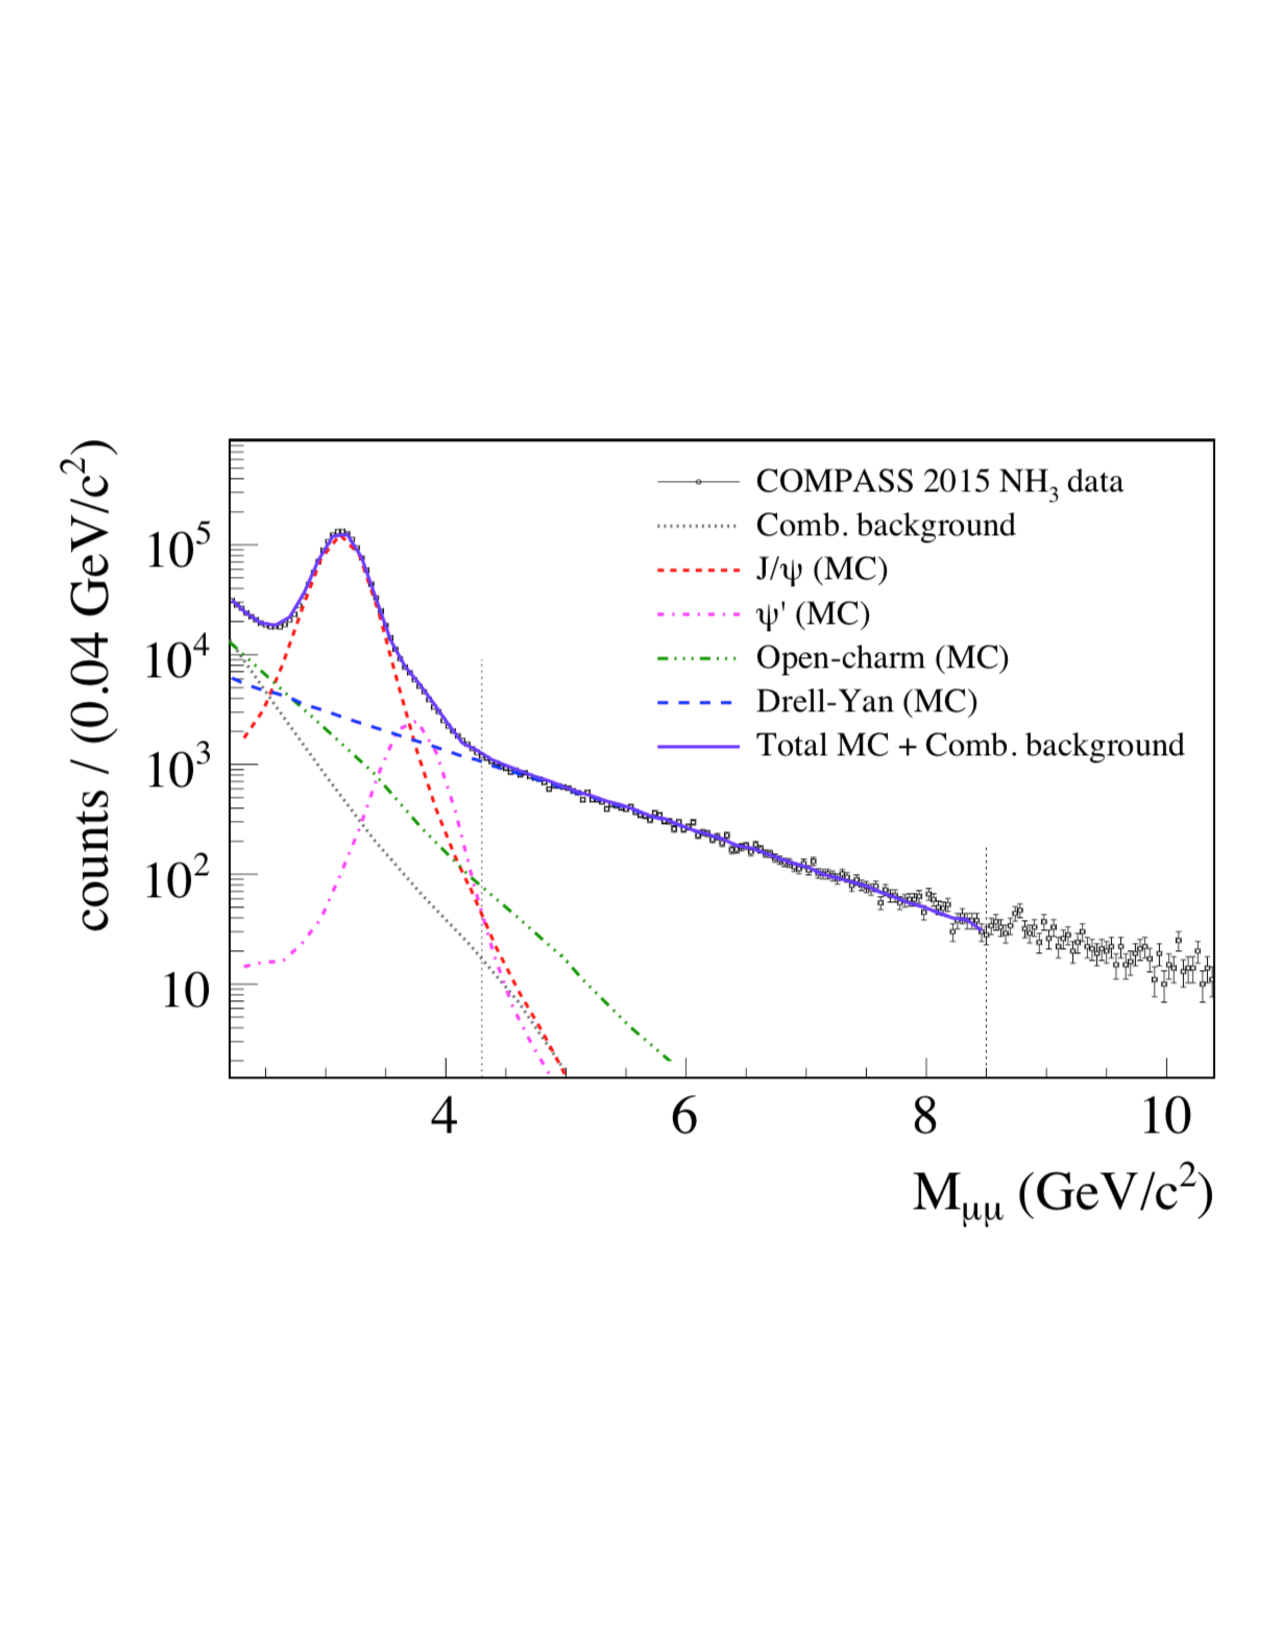
\includegraphics[width=0.6\textwidth,trim=1cm 7cm 1cm 7cm,
    clip]{DY_InvariantMass}
  \caption{The 2015 COMPASS invariant dimuon mass distribution and a fit to this
    data.  The data fit is from Monte-Carlo and combinatorial background
    analysis and is provided to show the background processes.  This image is
    taken from~\cite{compassDYpaper}.}
  \label{fig::DY_InvariantMass}
\end{figure}

Fig.~\ref{fig::DY_qT} shows the transverse virtual photon momentum, $q_T$,
distribution.  With the cut on $q_T$ between [0.4-5({\gvc})], the average $q_T$
is 1.2~{\gvc} while the average $M_{\mu\mu}$ is 5.3~{\gvcw}.  As stated in
chapter~\ref{ch::theory_exp}, the regime where TMD functions are the theoretical
model for parton distributions is when $q_T << M_{\mu\mu}$.  While the average
$q_T$ is less than the average $M_{\mu\mu}$, it is not excluded that the results
in this chapter are outside of the TMD regime.  Nevertheless all the results
presented in this chapter are determined assuming the TMD description is valid.

\begin{figure}[h!t]
  \centering
  \begin{subfigure}{0.45\textwidth}
    \centering 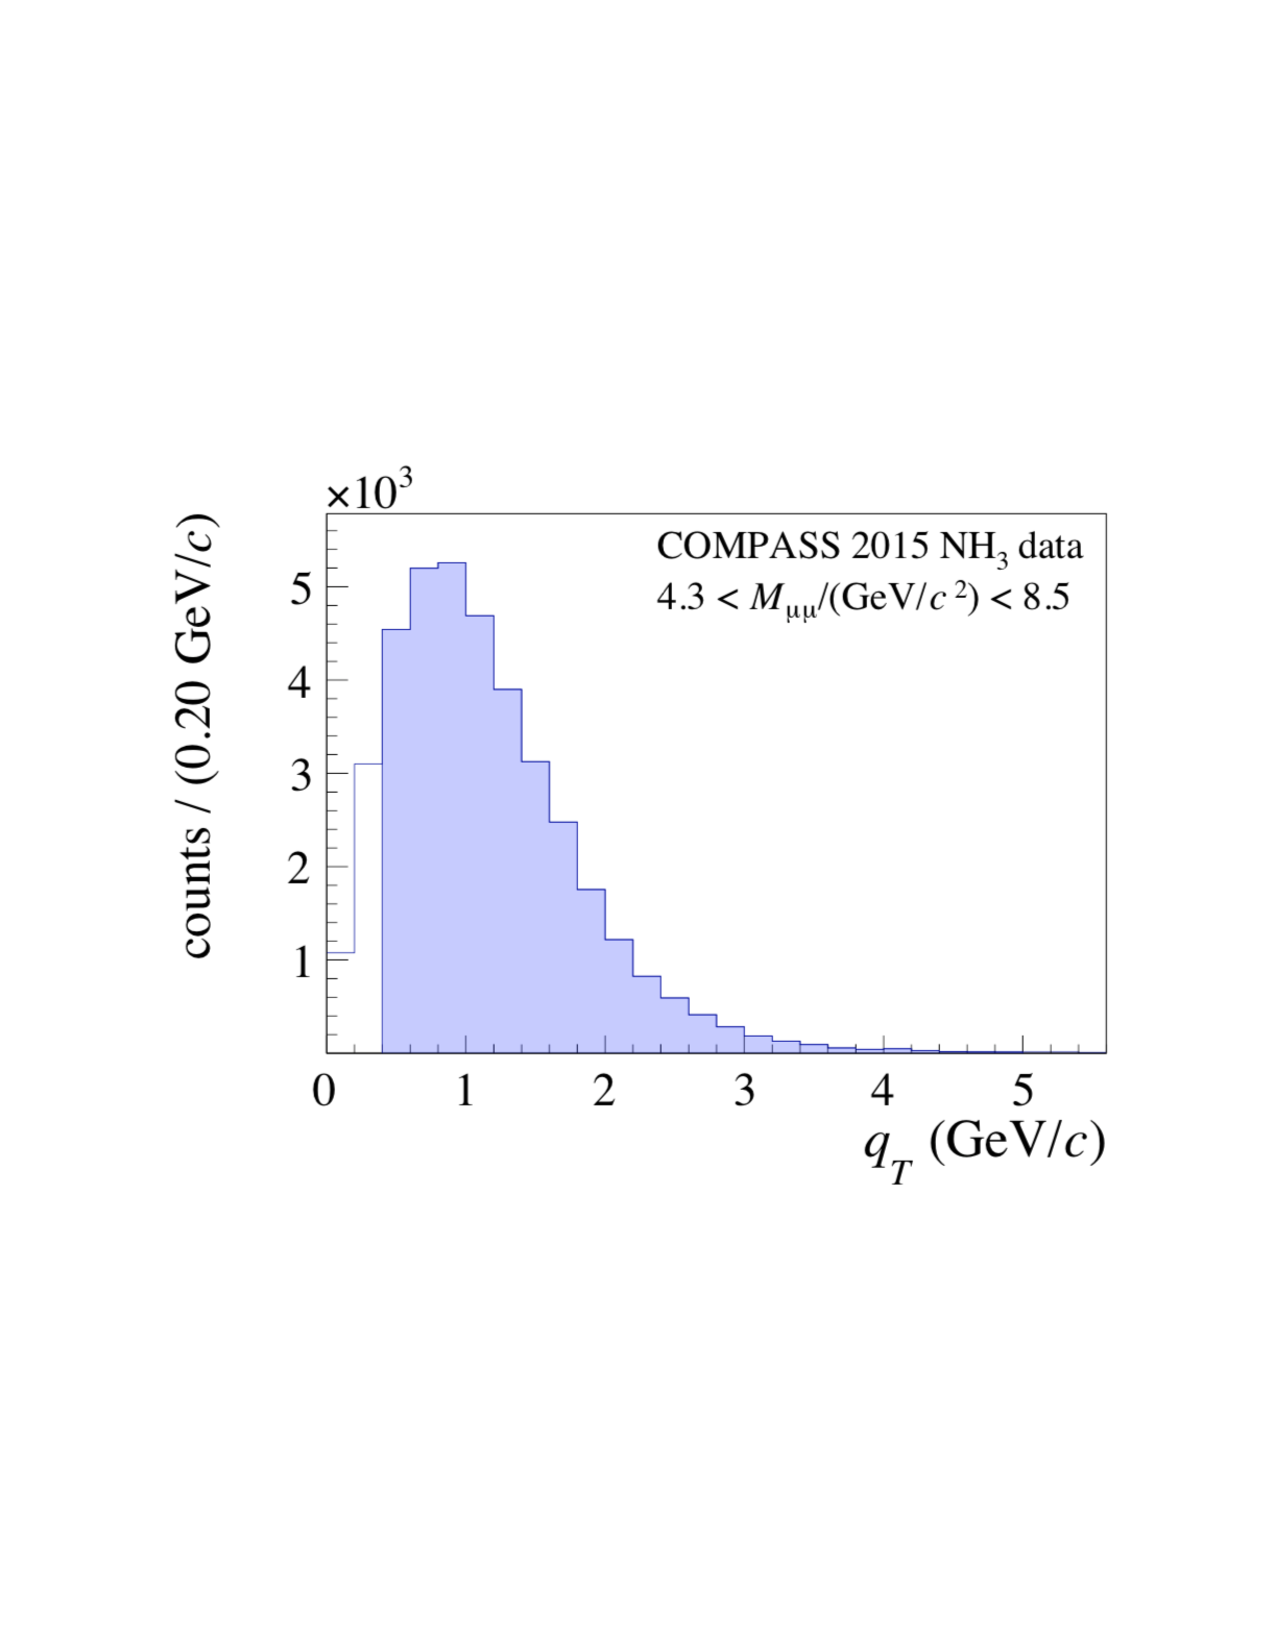
\includegraphics[width=\textwidth,trim=2cm 7.8cm 2cm 7cm,
      clip]{DY_qT}
    \caption{The $q_T$ distribution where the shaded region shows the data used
      in the high mass analysis and the unshaded region shows the full
      distribution without a $q_T$ cut.  This image is taken
      from~\cite{compassDYpaper}.}
    \label{fig::DY_qT}
  \end{subfigure}
  \begin{subfigure}{.02\textwidth}
    
\includegraphics[width=\linewidth]{tmp3}
    \label{fig::tmp3}%
  \end{subfigure}
    \begin{subfigure}{0.48\textwidth}
    \centering 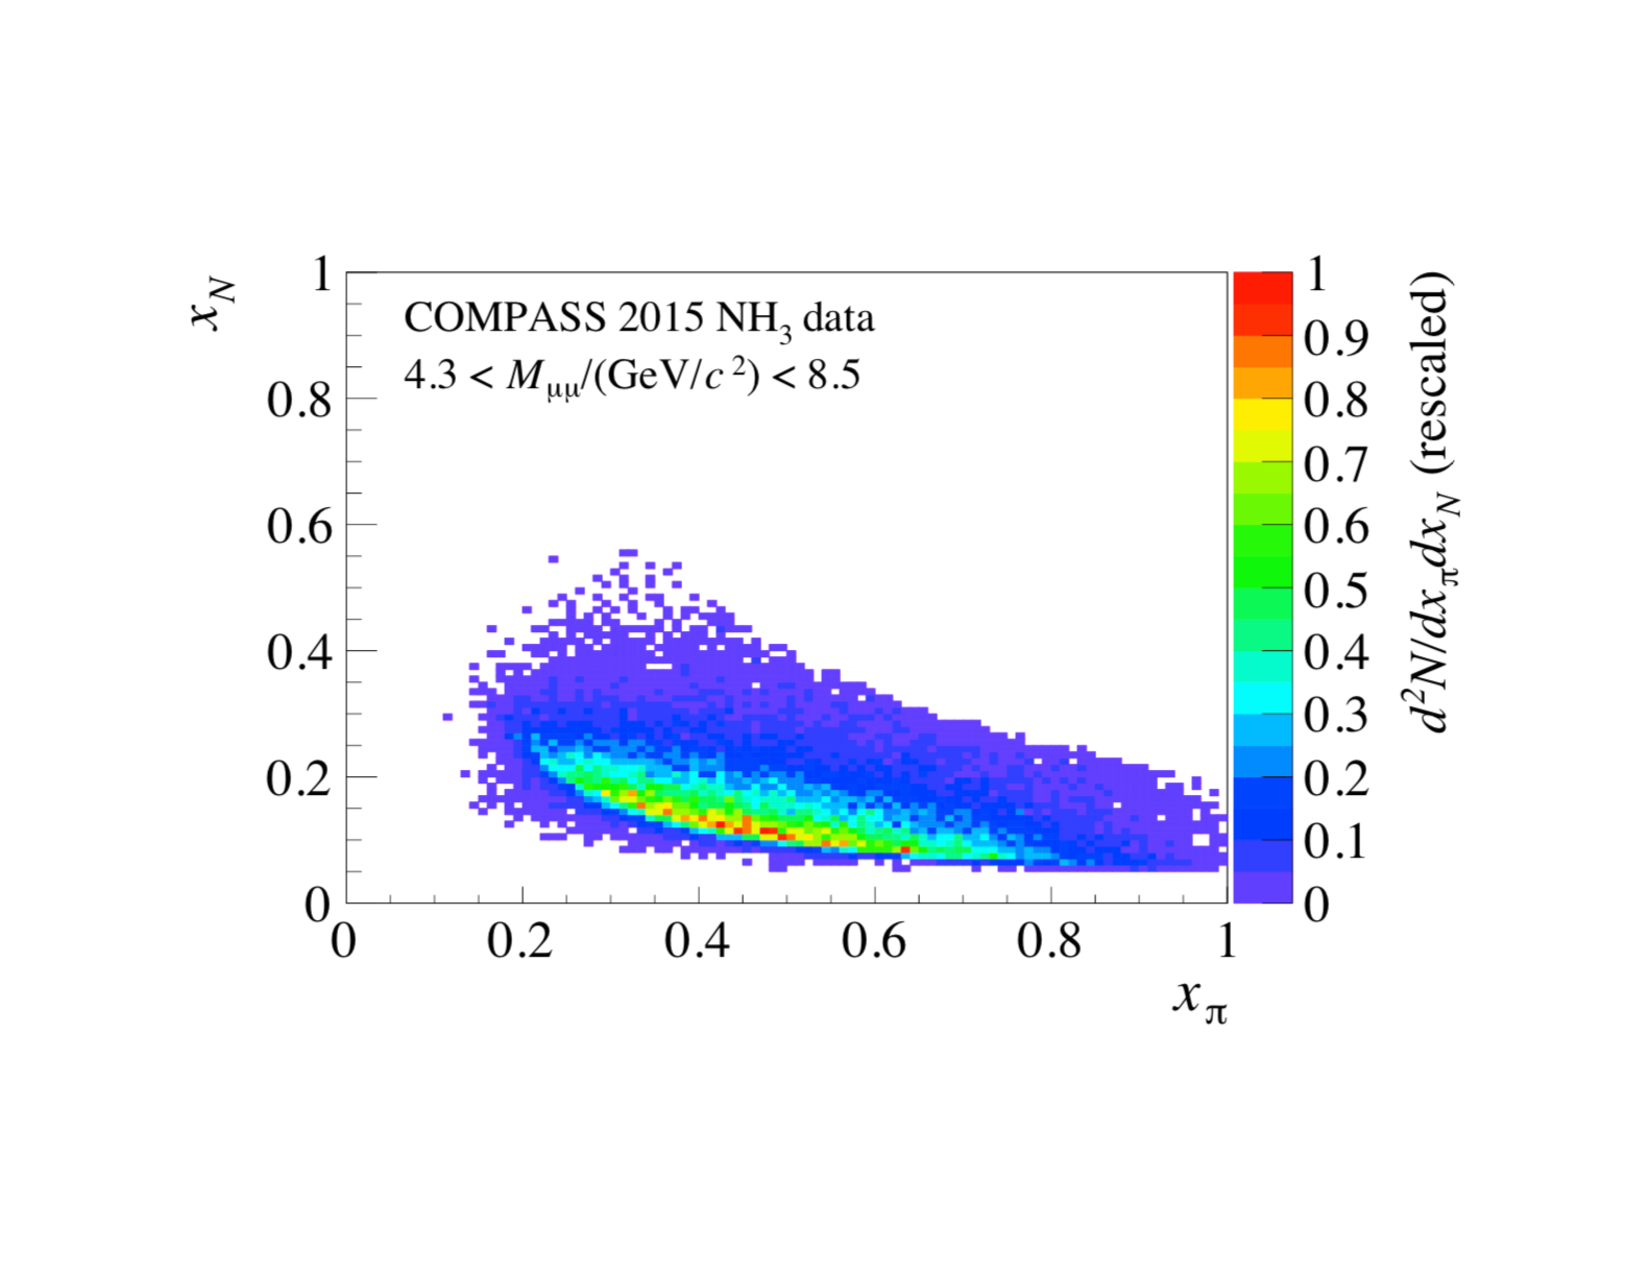
\includegraphics[width=\textwidth,trim=3.1cm 3.8cm 3.1cm
      3.8cm,clip]{DY_xPivxN}
    \caption{The 2-dimensional distribution of $x_{\pi}$ vs. $x_{N}$.  Both
      $x_{\pi}$ and $x_N$ are safely in their respective valence regions.  This
      image is taken from~\cite{compassDYpaper}.}
    \label{fig::DY_xPivxN}
  \end{subfigure}
\end{figure}

The distribution of $x_{\pi}$ versus $x_N$ is shown in
Fig.~\ref{fig::DY_xPivxN}.  The Bjorken-x of the proton, $x_N$, is almost
exclusively above 0.1 and as well Bjorken-x for the pion, $x_{\pi}$ is in its
valence region.  For these reasons it is safe to say that the Drell-Yan reaction
studied in the following analyses is the result of the pion's anti-u-quark
annihilating with the proton's u-quark.

The results from TSA analysis are determined from an extended unbinned maximum
likelihood fit to the data.  The virtual photon depolarization values are
determined on an event by event basis unlike the other analyses in this chapter.
The published integrated results of the 2015 data for the leading order and
sub-leading order TSAs are shown in Fig.~\ref{fig::DY_intAsymAmps}.  The leading
order TSAs are non-zero with approximate significance of: 1 sigma for the
Sivers TSA, $A_T^{\sin(\phi_S)}$, 1.2 sigma for the pretzelosity TSA,
$A_T^{\sin(2\phi_{CS}+\phi_S)}$ and 2 sigma for the transversity TSA,
$A_T^{\sin(2\phi_{CS}-\phi_S)}$.

\begin{figure}[h!t]
  \centering 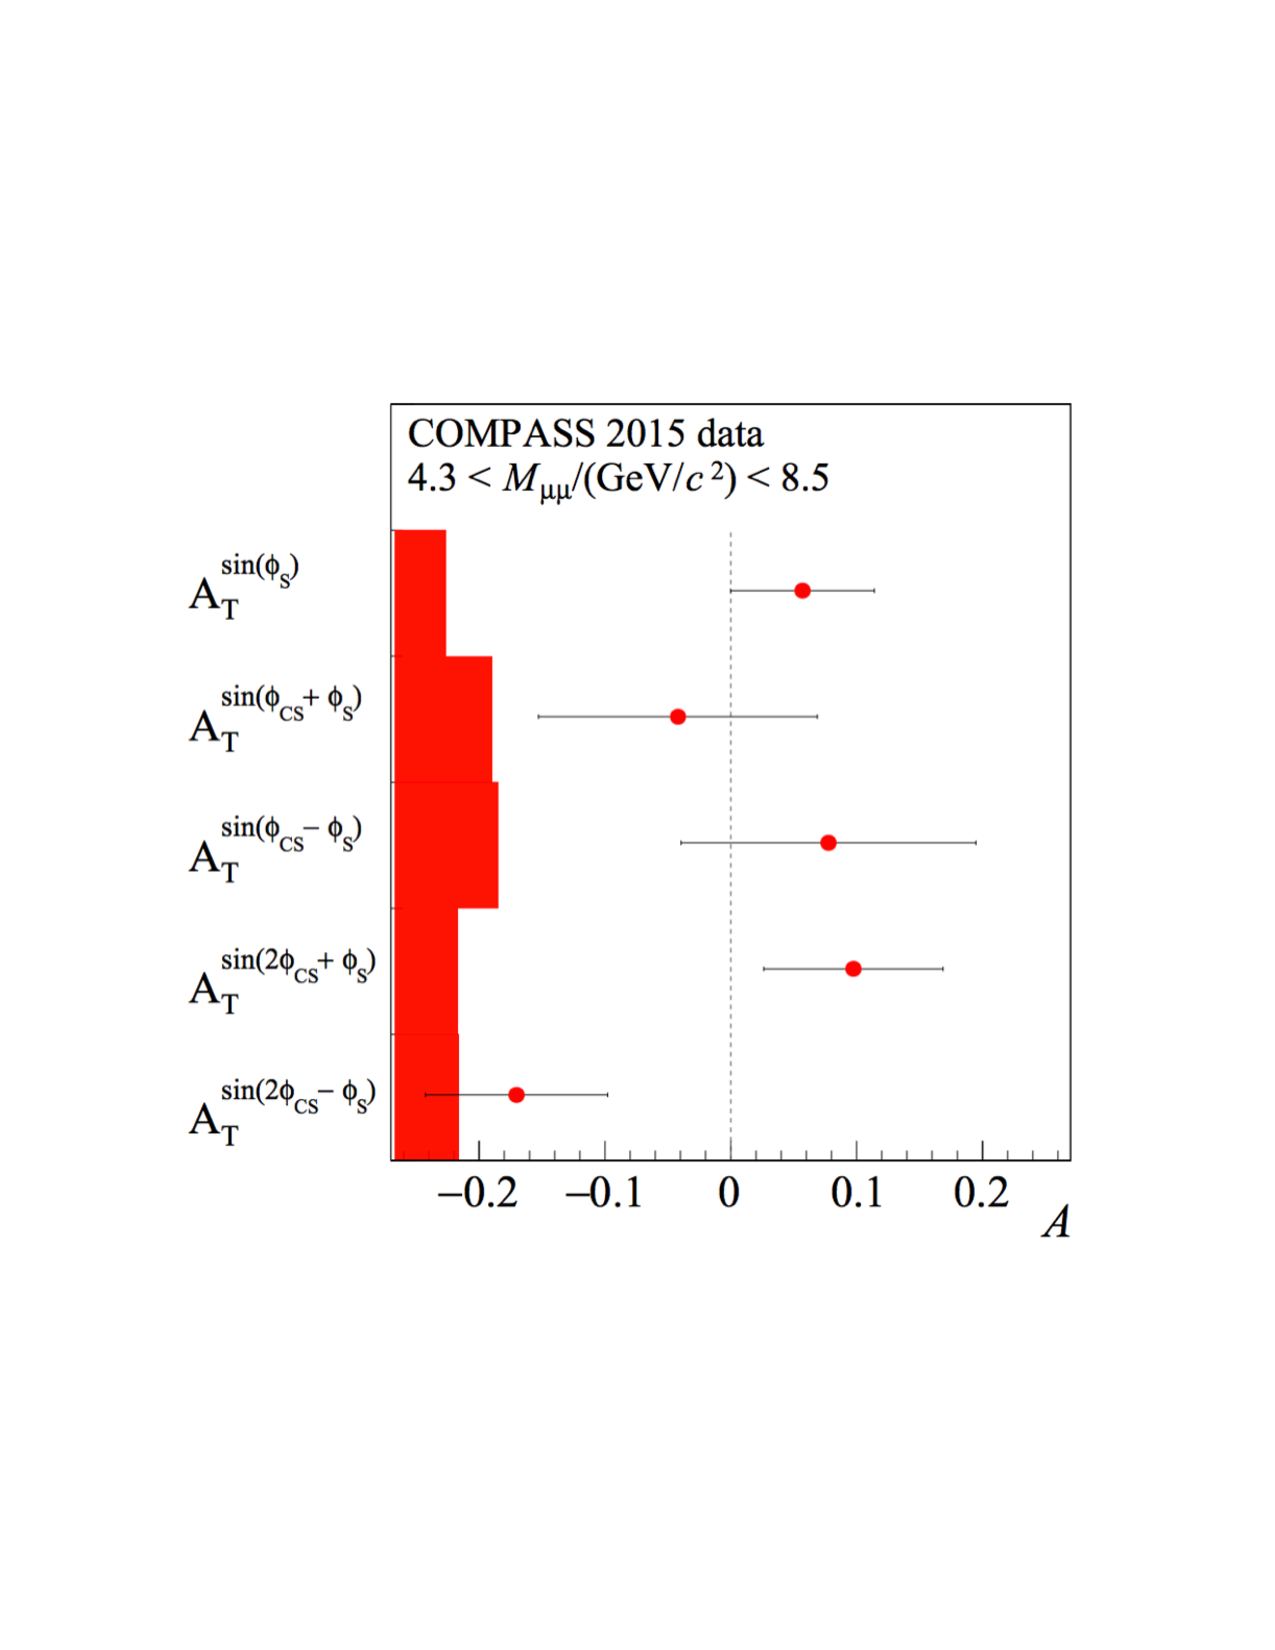
\includegraphics[width=0.43\textwidth,trim=3cm 7cm 3cm 6cm,
    clip]{DY_intAsymAmps}
  \caption{The integrated TSAs with statistical error bars and systematic
    uncertainty bands.  $A_T^{\sin(\phi_S)}$, $A_T^{\sin(2\phi_{CS}+\phi_S)}$,
    and $A_T^{\sin(2\phi_{CS}-\phi_S)}$ are leading order TSAs and
    $A_T^{\sin(\phi_{CS}+\phi_S)}$ and $A_T^{\sin(\phi_{CS}-\phi_S)}$ are
    sub-leading order TSAs.}
  \label{fig::DY_intAsymAmps}
\end{figure}

The comparison of the Sivers TSA, $A_T^{\sin(\phi_S)}$, with the expected sign
flip is shown in Fig.~\ref{fig::DY_Siv_signFlip}.  The positive solid theory
curves show the expected Sivers TSA assuming the Sivers function flips sign
between Drell-Yan and SIDIS.  The main difference in these three theory curves
is the $Q^2$ evolution which is also the main uncertainty in each prediction.
As can be seen the Sivers TSA is compatible with the expected sign change.
However, the error bars on the Sivers asymmetry amplitude are too large to
conclusively distinguish between the three theory curves or even to definitively
conclude on the sign change between Drell-Yan and SIDIS.  That being said, the
amplitude $A_T^{\sin(\phi_S)}$ is 2 sigma away from being incompatible with a
sign flip.

\begin{figure}[h!t]
  \centering 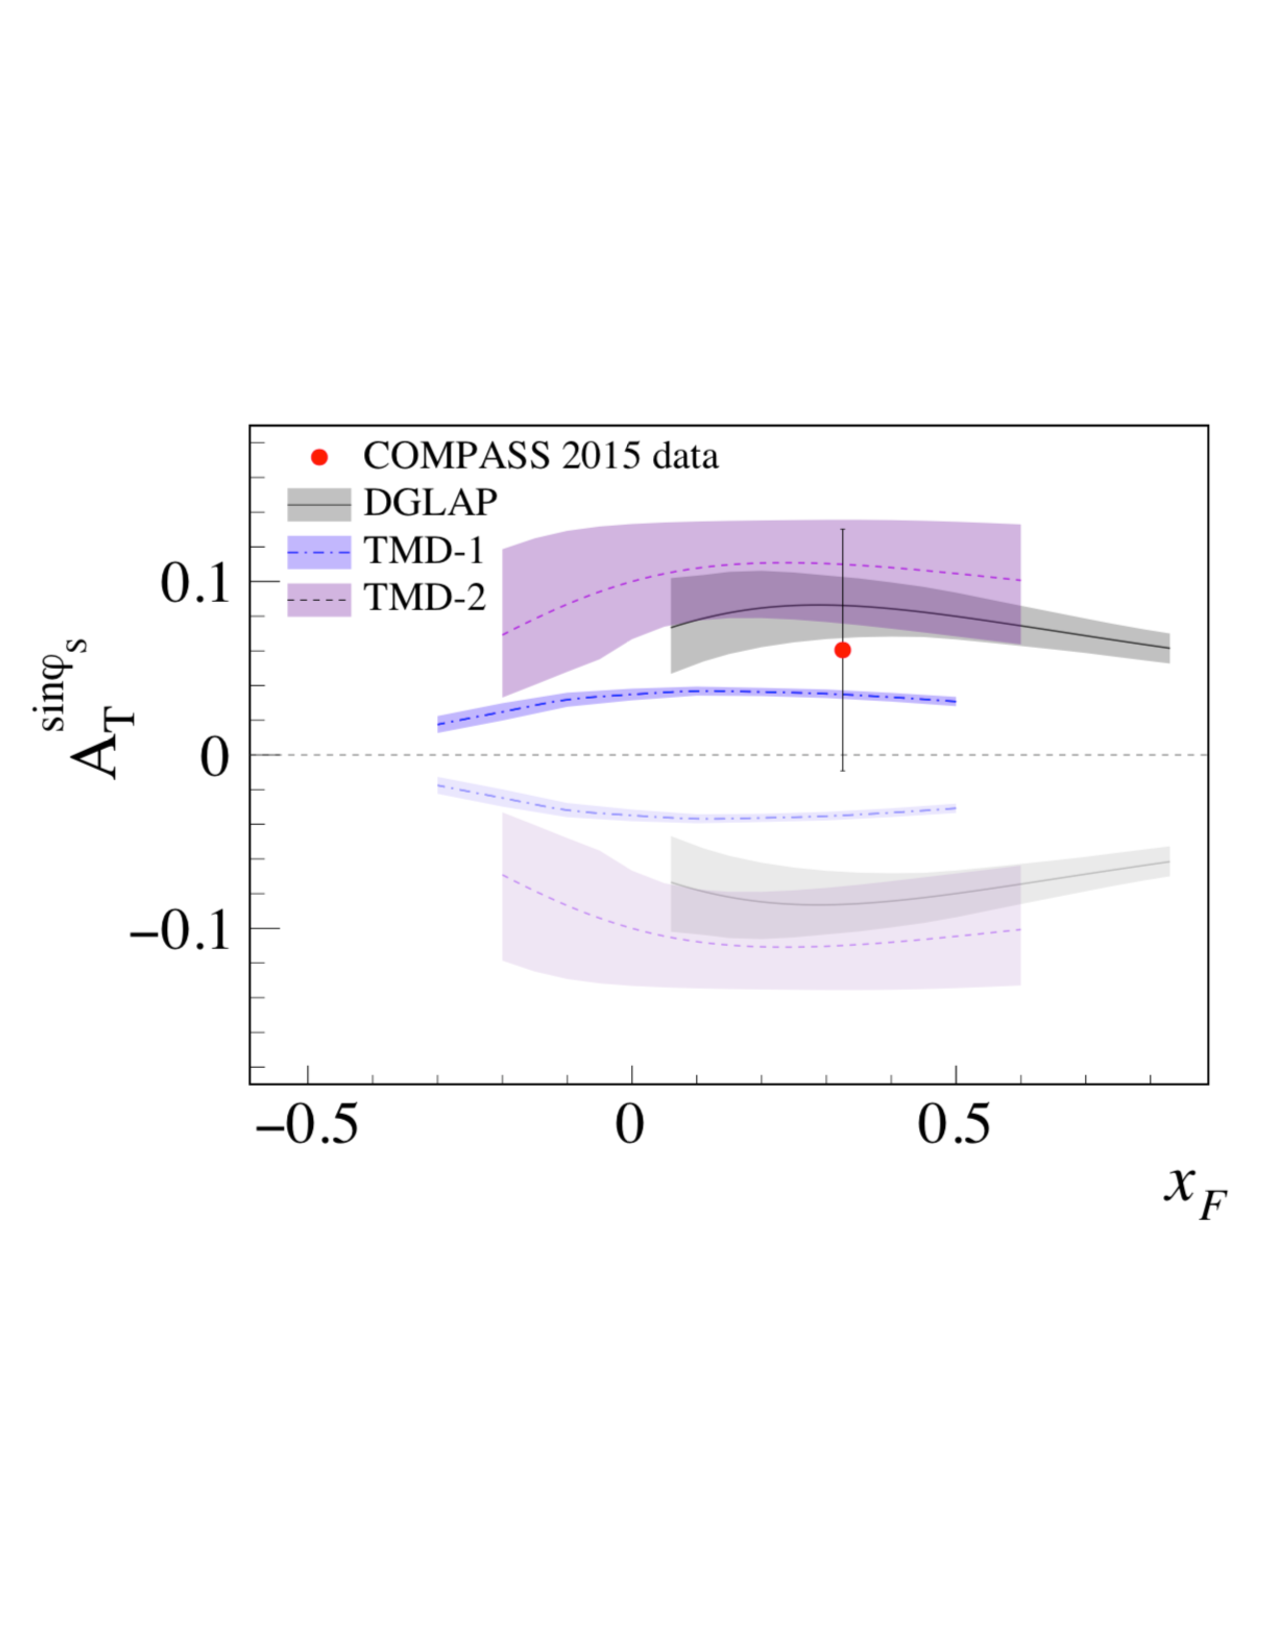
\includegraphics[width=0.6\textwidth, trim=0.5cm 7cm 0.5cm 7cm,
    clip]{DY_Siv_signFlip}
  \caption{The Sivers TSA along with theory curves for the expected sign change
    (sold curves) and without the sign change (opaque curves).  Theory curves
    and uncertainties are calculated using $Q^2$ evolution from
    DGLAP~\cite{Anselmino:2016uie}, TMD-1~\cite{Echevarria:2014xaa},
    TMD-2~\cite{Sun:2013hua}.  This image is taken from~\cite{compassDYpaper}.}
  \label{fig::DY_Siv_signFlip}
\end{figure}


\section{Double Ratio Analysis} \label{sec::doubleratio}
The double ratio method is used to determined spin-dependent asymmetry
amplitudes.  This means the asymmetry amplitudes $A^{\sin\phi_S}_T$,
$A^{\sin(2\phi+\phi_S)}_T$ and $A^{\sin(2\phi-\phi_S)}_T$ can be determined from
the 2015 transversely polarized Drell-Yan data.  The benefit of this method is
that the spectrometer acceptance does not effect the determination of the
asymmetry amplitudes.  The author of this thesis performed the analysis in this
section and found results consistent with those determined from TSA analysis.

\subsection{Asymmetry Extraction}
The double ratio is defined as

\begin{equation}
  R_D(\Phi) =
  \frac{N_1^{\uparrow}(\Phi)N_2^{\uparrow}(\Phi)}
       {N_1^{\downarrow}(\Phi)N_2^{\uparrow}(\Phi)},
\end{equation}
\noindent
where $N$ represents the counts, 1(2) is the upstream(downstream) target cell
and $\uparrow$($\downarrow$) denotes the transverse polarization direction.  The
number of counts, $N(\Phi)$, is defined as

\begin{equation}
  \label{equ::countsdef}
  N(\Phi) = L * \sigma(\Phi) * a(\Phi),
\end{equation}

\noindent
where $L$ is the luminosity, $\sigma$ is the cross-section and $a$ is the
spectrometer acceptance.  In Eq.~\ref{equ::countsdef} the acceptance is a
function of detector efficiencies and the spectrometer acceptance.  When
assuming the spin-dependent Drell-Yan cross-section,
Eq.~\ref{equ::DY_MostusefulXsect}, the number of counts, $N(\Phi)$, can be
written

\begin{equation}
  \label{equ::spindependentCounts}
  N(\Phi) = a(\Phi)L\sigma_U\Big(1 \pm D_{[\theta]}|S_T|A^w_T\sin(\Phi)\Big).
\end{equation}
\noindent
where +(-) is for target polarized up(down), $D_{[\theta]}$ is the virtual
photon depolarization factor and $|S_T|$ is the target polarization percentage.
The depolarization factor, $D_{[\theta]}$ is defined in
Eq.~\ref{equ::DYDepolarizationFactorDef}.  It can be thought of as the
probability for the virtual photon to decay and produce such an asymmetry
amplitude to that for a transversely polarized photon decay.  The target
polarization percentage, $|S_T|$ is defined as $fP$, where $f$ is the dilution
factor, Eq.~\ref{equ::dilution}, and $P$ is the target polarization percentage.
Therefore the double ratio can be written
\begin{align}
  R_D(\Phi) &= \frac{ a_1^{\uparrow}(\Phi)L_1^{\uparrow}\sigma_U\Big(1 +
    D_{[\theta]1}^{\uparrow}|S_{T1}^{\uparrow}|A^w_T\sin(\Phi)\Big)
    a_2^{\uparrow}(\Phi)L_2^{\uparrow}\sigma_U\Big(1 +
    D_{[\theta]2}^{\uparrow}|S_{T2}^{\uparrow}|A^w_T\sin(\Phi)\Big) } {
    a_1^{\downarrow}(\Phi)L_1^{\downarrow}\sigma_U\Big(1 -
    D_{[\theta]1}^{\downarrow}|S_{T1}^{\downarrow}|A^w_T\sin(\Phi)\Big)
    a_2^{\downarrow}(\Phi)L_2^{\downarrow}\sigma_U\Big(1 -
    D_{[\theta]2}^{\downarrow}|S_{T2}^{\downarrow}|A^w_T\sin(\Phi)\Big) }
  \\ \nonumber &= \Big(\frac{a_1^{\uparrow}(\Phi)a_2^{\uparrow}(\Phi)}
     {a_1^{\downarrow}(\Phi)a_2^{\downarrow}(\Phi)} \Big)
     \Big(\frac{L_1^{\uparrow}L_2^{\uparrow}}
         {L_1^{\downarrow}L_2^{\downarrow}}\Big)
         \frac{\Big(1+D_{[\theta]1}^{\uparrow}|S_{T1}^{\uparrow}|A^w_T\sin(\Phi)\Big)
           \Big(1+D_{[\theta]2}^{\uparrow}|S_{T2}^{\uparrow}|A^w_T\sin(\Phi)\Big)}
              {\Big(1-D_{[\theta]1}^{\downarrow}|S_{T1}^{\downarrow}|A^w_T\sin(\Phi)\Big)
                \Big(1-D_{[\theta]2}^{\downarrow}|S_{T2}^{\downarrow}|A^w_T\sin(\Phi)\Big)
              }.
\end{align}
\noindent
As is described in Sec~\ref{sec::datacollection}, the data is collected in two
week periods where the conditions of the spectrometer are frozen for each data
taking period.  For this reason the following reasonable acceptance assumption
is made
\begin{equation}
  \label{equ::a_resonable_assump}
  \frac{a_1^\uparrow(\Phi) a_2^\uparrow(\Phi)}
       {a_1^\downarrow(\Phi) a_2^\downarrow(\Phi)}
       = C.
\end{equation}
\noindent
where $C$ is a constant.  In addition
$L^{\downarrow(\uparrow)}_2$ = $rL^{\uparrow(\downarrow)}_1$ where $r$ is a
constant reduction factor and therefore the luminosity terms cancel out as
\begin{equation}
  \frac{L_1^{\uparrow}L_2^{\uparrow}}{L_1^{\downarrow}L_2^{\downarrow}}
  = \frac{L_1^{\uparrow}rL_1^{\downarrow}}{L_1^{\downarrow}rL_1^{\uparrow}}
  = 1.
\end{equation}
\noindent
Finally the asymmetry amplitudes and target polarizations are assumed to be
small so the double ratio can be simplified to

\begin{align}
  R_D(\Phi) &=
  C\frac{\Big(1+D_{[\theta]1}^{\uparrow}|S_{T1}^{\uparrow}|A^w_T\sin(\Phi)\Big)
    \Big(1+D_{[\theta]2}^{\uparrow}|S_{T2}^{\uparrow}|A^w_T\sin(\Phi)\Big)}
  {\Big(1-D_{[\theta]1}^{\downarrow}|S_{T1}^{\downarrow}|A^w_T\sin(\Phi)\Big)
    \Big(1-D_{[\theta]2}^{\downarrow}|S_{T2}^{\downarrow}|A^w_T\sin(\Phi)\Big)}
  \\ \nonumber &\approx
  C\frac{1+\Big[D_{[\theta]1}^{\uparrow}|S_{T1}^{\uparrow}|+D_{[\theta]2}^{\uparrow}|S_{T2}^{\uparrow}|\Big]
    A^w_T\sin(\Phi)}
  {1-\Big[D_{[\theta]1}^{\downarrow}|S_{T1}^{\downarrow}|+D_{[\theta]2}^{\downarrow}|S_{T2}^{\downarrow}|\Big]
    A^w_T\sin(\Phi)} \\ \nonumber &\approx
  C\Big(1+\Big[D_{[\theta]1}^{\uparrow}|S_{T1}^{\uparrow}|+D_{[\theta]2}^{\uparrow}|S_{T2}^{\uparrow}|\Big]
  A^w_T\sin(\Phi)\Big)\Big(1+\Big[D_{[\theta]1}^{\downarrow}|S_{T1}^{\downarrow}|+D_{[\theta]2}^{\downarrow}|S_{T2}^{\downarrow}|\Big]
  A^w_T\sin(\Phi)\Big) \\ \nonumber &\approx C\Big(1 +
  \Big[D_{[\theta]1}^{\uparrow}|S_{T1}^{\uparrow}|+D_{[\theta]2}^{\uparrow}|S_{T2}^{\uparrow}|+D_{[\theta]1}^{\downarrow}|S_{T1}^{\downarrow}|+D_{[\theta]2}^{\downarrow}|S_{T2}^{\downarrow}|\Big]A^w_T\sin(\Phi)\Big).
\end{align}
\noindent
Then making the assumption that the polarizations, $S_T$, and the virtual photon
depolarization factors, $D_{\Phi}$ are approximately constant throughout a data
period, the asymmetry amplitude of interest can be determined by fitting the
double ratio with the function
\begin{equation}
  \label{equ::dr_fit_formula}
  f(\Phi) = [p0](1+4[p1]\sin(\Phi),
\end{equation}
\noindent
where $[p0]$ and $[p1]$ are fit parameters and $[p1]$ represents the asymmetry
amplitude of interest.  The $[p1]$ parameter is later corrected for average
polarization and virtual photon depolarization factors.

The double ratio, $R_D$, is determine as a function of $\Phi$, where the angle
$\Phi$ depends on which asymmetry amplitude is being determined.  The assumption
made in the measured counts formula, Eq.~\ref{equ::spindependentCounts}, is that
all angles except the spin-dependent $\Phi$ angle are integrated over.  When
this is the true, all the Drell-Yan cross-section fourier components integrate
to zero except the constant term.  The following table,
Table~\ref{tab::ratio_phiAngles}, list which $\Phi$ angle is used to determine
which spin-dependent asymmetry amplitude.

\begin{table}[h!t]
  \centering
  \caption{Measured counts as a function of each $\Phi$ angle}
  \begin{tabular}{ |c|c|c|c| }
    \hline \textbf{Asymmetry Amplitude}& \textbf{Corresponding TMD Function}&
    \textbf{$\Phi$ Angle}& \textbf{$\Phi$ Range (radians)} \\ \hline
    
    $A^{\sin(\phi_S)}_T$& Sivers& $\phi_S$& [-$\pi$, $\pi$] \\ \hline

    $A^{\sin(2\phi-\phi_S)}_T$& Transversity& $2\phi-\phi_S$& [-3$\pi$, 3$\pi$]
    \\ \hline

    $A^{\sin(2\phi+\phi_S)}_T$& Pretzelosity& $2\phi+\phi_S$& [-3$\pi$, 3$\pi$]
    \\ \hline
  \end{tabular}
    \label{tab::ratio_phiAngles}
\end{table}

The variance of the double ratio, assuming Poisson counting statistics, is

\begin{equation}
  \sigma^2_{R_D} = R^2_D(\Phi)\Big(\frac{1}{N_1^\uparrow(\Phi)}
    + \frac{1}{N_2^\uparrow(\Phi)}
    + \frac{1}{N_1^\downarrow(\Phi)}
    +\frac{1}{N_2^\downarrow(\Phi)}
   \Big).
\end{equation}

\subsection{Results}\label{sec::doubleratio_results}
The results of the asymmetry amplitudes are determined in each of the nine
periods and then combined as a weighted average.  The asymmetries are calculated
this way to minimize the effects of acceptance changes between periods as the
spectrometer was kept stable within each period but had the options for detector
changes and repairs between periods.  As well this weighted average method
allows for future measurements to be combined as a weighted average with the
final overall results without the need to know individual period results.  This
resulting asymmetry amplitudes are determined from a weighted average as
\begin{equation}
  \label{equ::wAvg}
  A = \frac{
    \sum_{period}
  A_{period}\sigma^{-2}_{period}
  }{
    \sum_{period} \sigma^{-2}_{period}
    },
  \quad \delta A = \sqrt{\sum_{period}
  \frac{1}{\sigma^{-2}_{period}}}.
\end{equation}

For each period and each kinematical bin, the asymmetry is determined by fitting
the double ratio and with Eq.~\ref{equ::dr_fit_formula}.  The results of the fit
actually determines the quantity

\begin{equation}
  A^w_T \langle D_{[\theta]} \rangle \langle |S_T|\rangle.
\end{equation}
\noindent
The asymmetry amplitude is ultimately determined by dividing the fit results by
the average polarization and average virtual photon depolarization values per
period.

To determine the asymmetry amplitude, the double ratio is binned in eight bins
in $\Phi$.  Eight bins are chosen due to the low statistics from Drell-Yan data.
Fig.~\ref{fig::dr_example_trans} shows an example of the binned double ratio and
fit results.

\begin{figure}[h!t]
  \centering 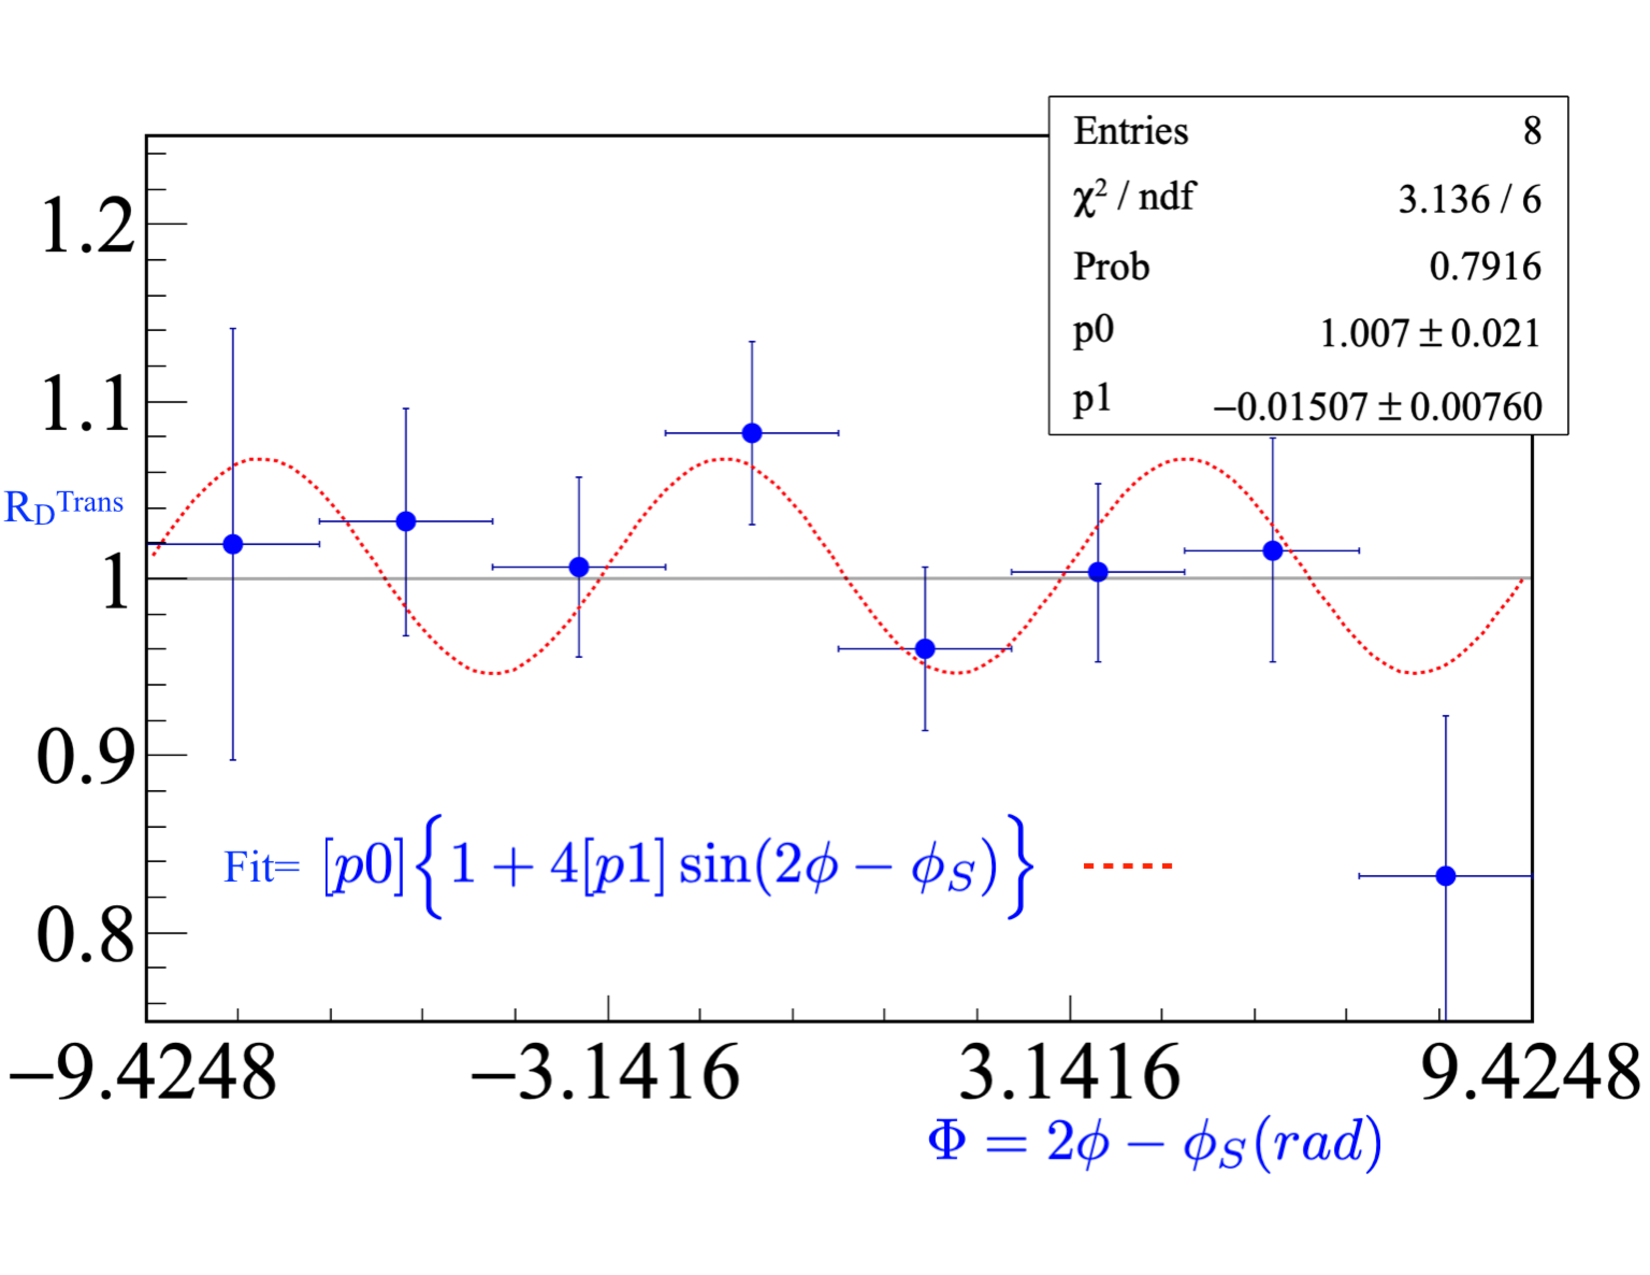
\includegraphics[width=0.6\textwidth,trim=0cm 1cm 0cm 1cm,
    clip]{dr_example_trans}
  \caption{An example double ratio and corresponding fit (red) to determine the
    amplitude $A_T^{\sin(2\phi-\phi_S)}$}
  \label{fig::dr_example_trans}
\end{figure}

\noindent
The results for all the spin-dependent asymmetry amplitudes are shown in
Fig.~\ref{fig::dr_final_results}.  As can be seen, the significance of the
integrated asymmetry amplitudes is: over 1 sigma above zero for the Sivers,
$A^{\sin\phi_S}_T$, over 3 sigma above zero for Preztelosity,
$A^{\sin(2\phi+\phi_S)}_T$, and 3 sigma below zero for transversity,
$A^{\sin(2\phi-\phi_S)}_T$.

\begin{figure}[h!t]
  \centering 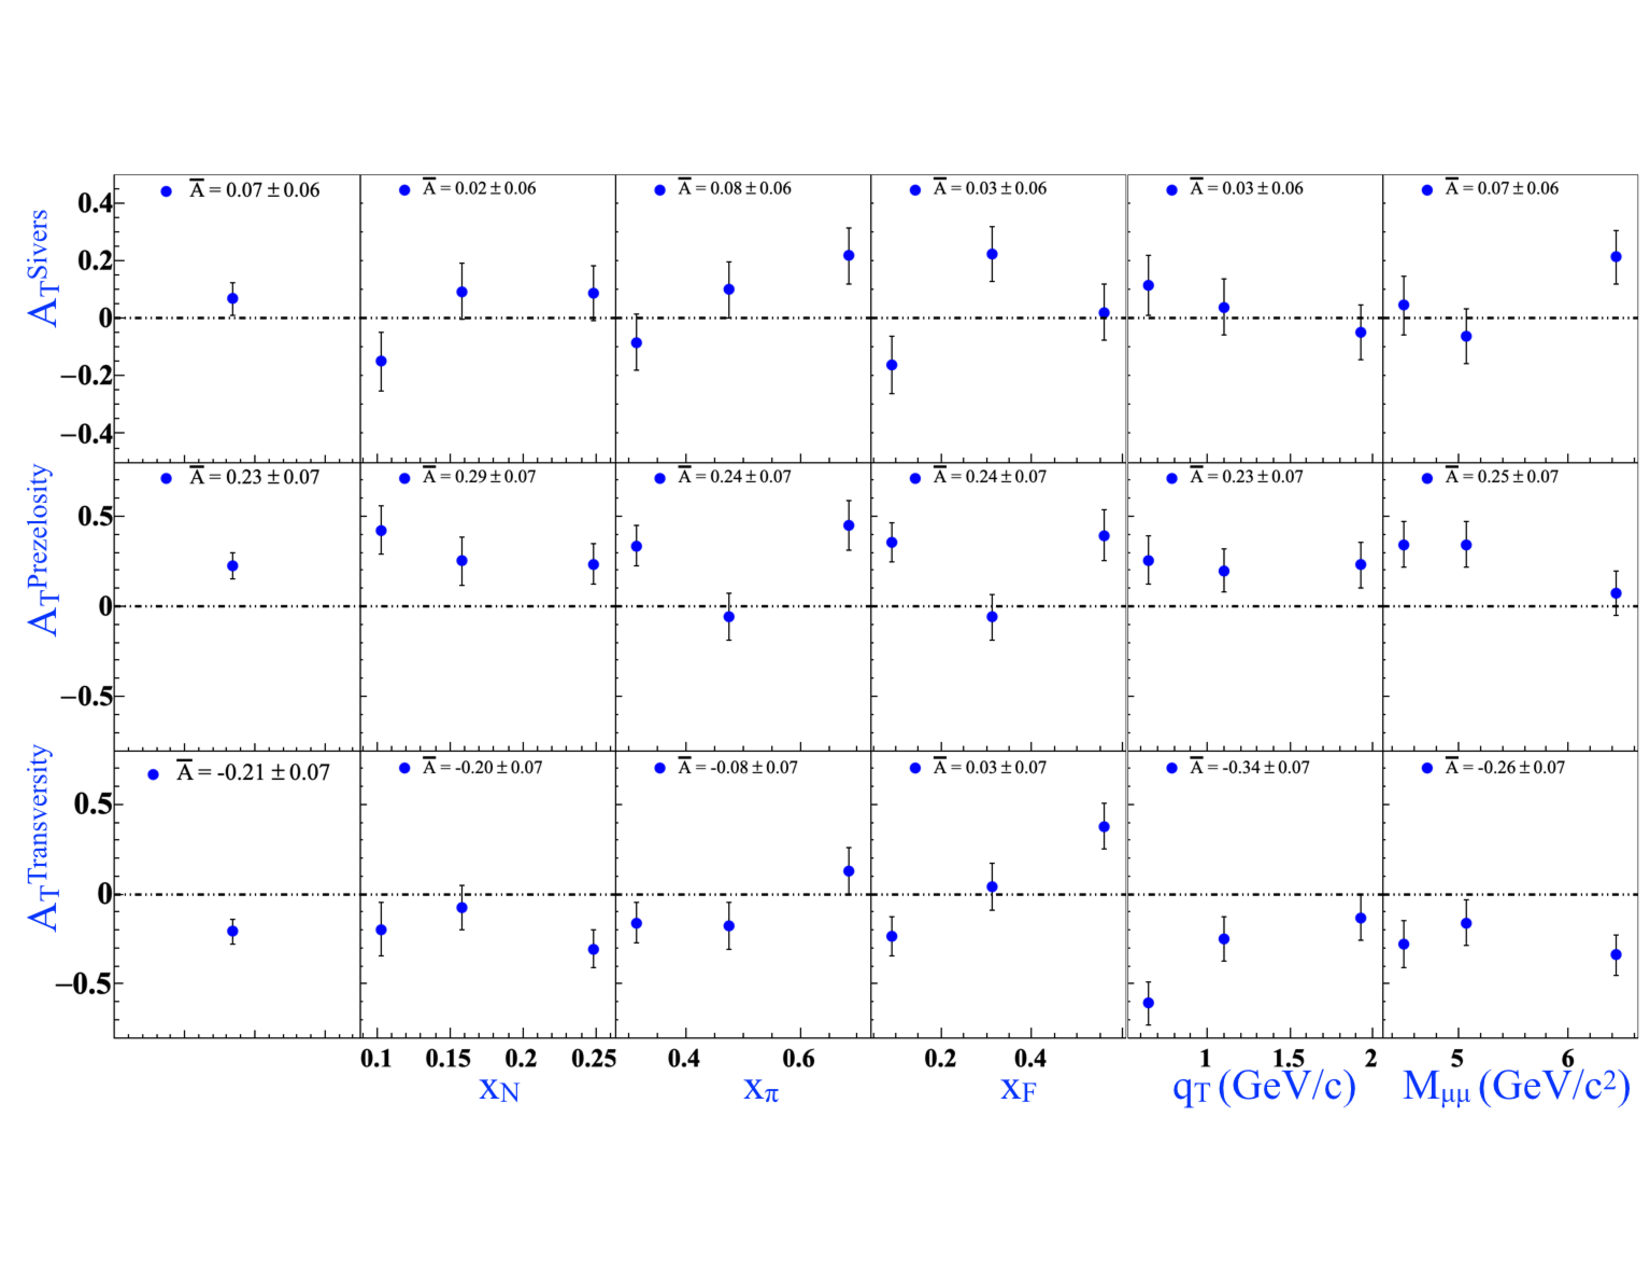
\includegraphics[width=\textwidth,trim=0cm 2.5cm 0cm 2.5cm,
    clip]{dr_final_results}
  \caption{The results and statistical error bars for the transverse
    spin-dependent asymmetry amplitudes $A^{\sin\phi_S}_T$ (top),
    $A^{\sin(2\phi+\phi_S)}_T$ (middle) and $A^{\sin(2\phi-\phi_S)}_T$ (bottom)
    determined from the double ratio method.}
  \label{fig::dr_final_results}
\end{figure}


\section{$q_T$-Weighted Asymmetries} \label{sec::qtweighted}
The $q_T$ weighted asymmetries analysis is used to determine three asymmetry
amplitudes related to TMD functions.  This analysis determined the three
amplitudes: $A_T^{\sin(\phi_S) q_T/M_N}$, $A_T^{\sin(2\phi+\phi_S)
  q^3_T/(2M_{\pi}M_N^2)}$ and $A_T^{\sin(2\phi-\phi_S) q_T/M_{\pi}}$ which are
related to the Sivers, Preztelosity and transversity TMD PDFs respectively.

The theoretical introduction and motivation for measuring $q_T$-weighted
asymmetries is provided in Sec~\ref{sec::qt_w_theory}.  The author of this
thesis was a cross checker for the $q_T$-weighted asymmetry results which is a
required step for any results to become public.  For the full details of the
$q_T$-weighted analysis see reference~\cite{janthesis}.

\subsection{Event Selection}
The results for this analysis were released prior to the slot1 reconstruction
production and therefore this analysis uses the t3 reconstruction.  For
$q_T$-weighted asymmetries the results depend on the full range of the $q_T$
distribution.  In the other analyses in this chapter however, a cut was placed
on high and low $q_T$ values to ensure better azimuthal angular resolution and
quality reconstructed events.  This cut cannot be applied for $q_T$-weighted
analysis because it will effect the weighting used to determine the asymmetry
amplitudes.  On the other hand the combinatorial background and badly
reconstructed events from the high $q_T$ phase space should be cut.  The next
section goes into the details and the remedy for a $q_T$ related cut. All of the
other cuts from Sec~\ref{sec::dy_eventselection} are the same except for this
$q_T$ cut. Figure~\ref{tab::qt_EventTable} provides the final cut order and the
remaining statistics after each cut for this $q_T$-weighted analysis.

\subsubsection{High $q_T$} \label{sec::high_qt}
The $q_T$ distribution without any $q_T$ cuts is shown in
Fig.~\ref{fig::qT_noCuts}.  As can be seen the $q_T$ distribution reaches values
much higher than the maximum 5~{\gvc} cut from the other analyses in this
chapter.  The most fundamental problem with this $q_T$ distribution is that some
of the events violate conservation of momentum.  A first remedy to the high
$q_T$ values then is to add a cut which demands momentum conservation.  This is
achieved by demanding that the momentum sum of the detected muons is physically
possible, $\ell^+ \; + \; \ell^- \; < \; 190$~GeV/c.  Note that this cut does
not take into account the momentum spread of the beam due to the fact that the
beam momentum spread is expected to be small.  Fig.~\ref{fig::qT_PconserveCut}
shows how this cut affects the $q_T$ distribution.  As can be seen, $q_T$ still
reaches values much higher than the 5~GeV/c cut from the other TMD analyses.
The remaining high $q_T$ events still have the potential to be poorly
reconstructed events or combinatorial background and for this reason an
additional cut was put on the individual muons transverse momentum such that
$\ell_T^{\pm} \; <$ 7~GeV/c.

\begin{figure}[h!t]
  \centering
  \begin{subfigure}{.46\textwidth}
    \centering 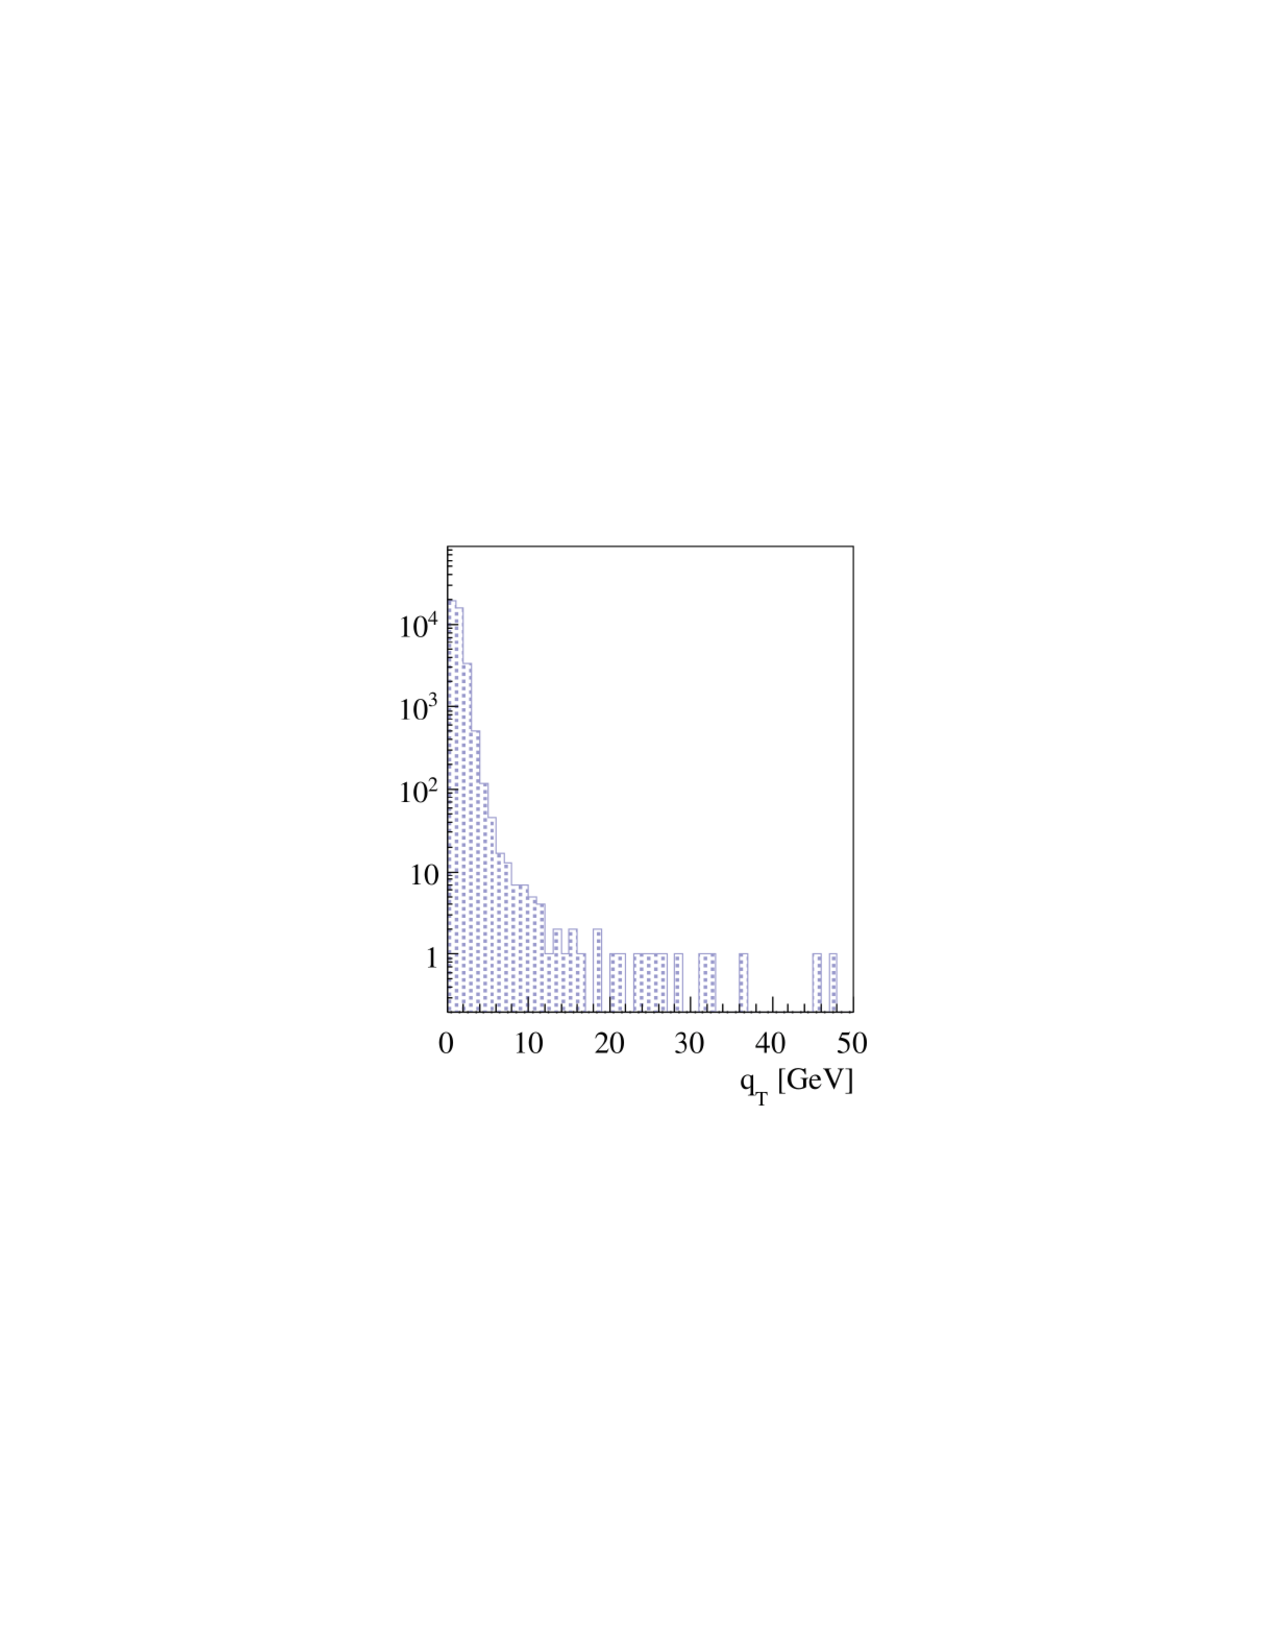
\includegraphics[width=\linewidth, trim=6cm 8.7cm 6cm 8cm,
      clip]{qT_noCuts}
    \caption{$q_T$ distribution without cuts on $q_T$.  All other cuts expect
      the $q_T$ cut from Sec~\ref{sec::dy_eventselection} are applied.  This
      image is from~\cite{janthesis}}
    \label{fig::qT_noCuts}
  \end{subfigure}%
  \begin{subfigure}{.02\textwidth}
    \centering
    
\includegraphics[width=\linewidth]{tmp2}
    \label{fig::tmp2}%
  \end{subfigure}
  \begin{subfigure}{.46\textwidth}
    \centering 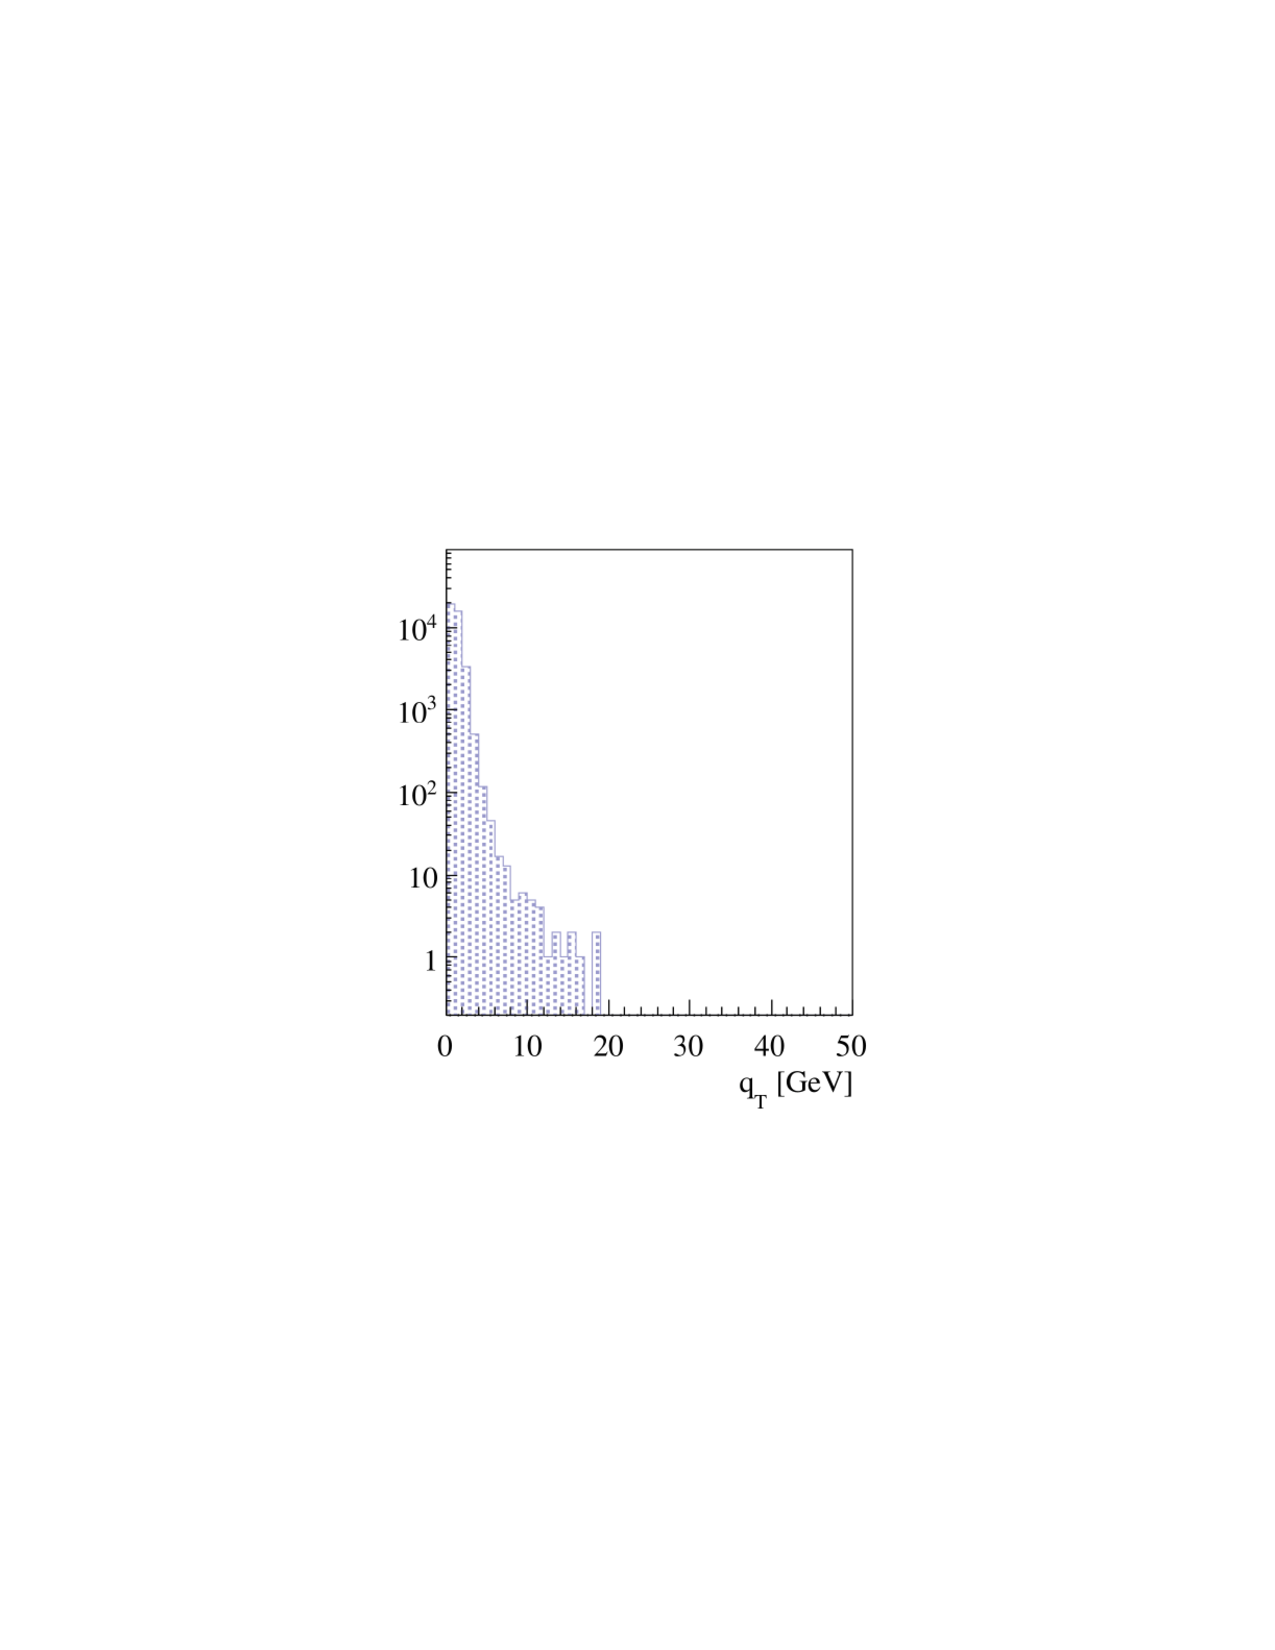
\includegraphics[width=\linewidth, trim=6cm 9cm 6cm 8cm,
      clip]{qT_PconserveCut}
    \caption{$q_T$ distribution after the momentum conservation cut is added,
      $\ell^+ \; + \; \ell^- \; < \; 190$ GeV/c.  All other cuts expect the
      $q_T$ cut from Sec~\ref{sec::dy_eventselection} are applied.  This image
      is from~\cite{janthesis}}
    \label{fig::qT_PconserveCut}
  \end{subfigure}
\end{figure}

\begin{figure}[h!t]
  \centering
    \begin{tabular}{ |c|c|c| }
      \hline \textbf{Cuts}& \textbf{Events} & \textbf{\% Remaining} \\ \hline

      \multirow{2}{15em}{$\mu^+\mu^-$ from best primary vertex,
        4.3$<M_{\mu\mu}<8.5$ GeV/c$^2$}& 1,159,349& 100.00\\ & & \\ \hline
      
      \multirow{2}{14em}{Triggers: (2LAS or LASxOT) and not LASxMiddle}& 
      868,291& 74.89\\ & & \\ \hline
      
      Z$_{first} <$ 300 cm, Z$_{last} >$ 1500 cm& 784,379& 67.66\\ \hline

      $\Delta$t defined& 776,643& 66.99\\ \hline
      
      $|\Delta\mathrm{t}| <$ 5 ns& 337,081& 32.18\\ \hline

      $\chi^2_{track}$/ndf $<$ 10& 370,054& 31.92\\ \hline

      $\ell^+ + \ell^- < 190$ GeV/c& 219,304& 18.92\\ \hline

      $\ell_T^\pm < 7$ GeV/c& 219,014& 18.89\\ \hline

      Trigger Validation& 168,939& 14.57\\ \hline

      Good Spills& 137,812& 11.89\\ \hline

      0$<$ x$_{\pi}$ x$_N$ $<$1, -1$<$ x$_F$ $<$1& 137,802& 11.89  \\ \hline

      Z Vertex within NH$_3$& 42,646& 3.68\\ \hline

      Vertex Radius $<$ 1.9cm& 39,088& 3.37\\ \hline

    \end{tabular}
    \caption{Event selection statistics for $q_T$-weighed asymmetry analysis
      from all periods combined}
    \label{tab::qt_EventTable}
\end{figure}

\subsection{Binning}
As with the other analyses in this chapter, the asymmetry is determined in bins
of the Drell-Yan physical kinematic variables: $x_N$, $x_\pi$, $x_F$,
$M_{\mu\mu}$ and an overall integrated value.  No $q_T$ binning is used however,
because a full integration of the $q_T$ variable needs to be taken into account
to form the weighted asymmetry.

\subsection{Asymmetry Method}
The weighted asymmetry amplitudes $A_T^{\sin(\phi_S) q_T/M_N}$,
$A_T^{\sin(2\phi+\phi_S) q^3_T/(2M_{\pi}M_N^2)}$ and $A_T^{\sin(2\phi-\phi_S)
  q_T/M_{\pi}}$ are determined using a modified double ratio.  As with the
double ratio method from Sec~\ref{sec::doubleratio}, the modified double ratio
does not depend on the spectrometer acceptance.  The modified double ratio is
defined as

\begin{equation}
  \label{equ::modified_dr}
  R^W_{DM}(\Phi)=
  \frac{N^{\uparrow W}_{1}N^{\uparrow W}_{2}
    - N^{\downarrow W}_{1}N^{\downarrow W}_{2}}
       {\sqrt{(N^{\uparrow W}_{1}N^{\uparrow W}_{2}
         + N^{\downarrow W}_{1}N^{\downarrow W}_{2})
         (N^{\uparrow}_{1}N^{\uparrow}_{2}
         + N^{\downarrow}_{1}N^{\downarrow}_{2})}},
\end{equation}
\noindent
where similar notation is used from the previous analyses where
$\uparrow$($\downarrow$) is the transverse polarization direction, 1(2) denotes
the upstream(downstream) cell, $N^{W}$ is the weighted counts, $W$ is the weight
used and $N$ denotes the unweighted counts.  The angles $\Phi$, in the modified
double ratio, are the same used for the double ratio,
Table~\ref{tab::ratio_phiAngles}, and give access to asymmetry amplitudes
related to the same corresponding TMD functions.  Under the same reasonable
acceptance ratio assumption, Eq.~\ref{equ::a_resonable_assump}, from the double
ratio method the acceptance cancels out in the double ratio method.  Using this
assumption, the modified double ratio reduces to

\begin{equation}
  \label{equ::dr_fit_form}
  R^W_{DM}(\Phi) \approx 2 \tilde{D}_{\sin\Phi}\langle S_T \rangle
  A_T^{\sin(\Phi)W} \sin\Phi,
\end{equation}
\noindent
where $\tilde{D}_{\sin\Phi}$ is an integrated virtual photon depolarization
factor defined as

\begin{equation}
  \tilde{D}_{\sin\phi_S} = 1, \quad\quad \tilde{D}_{\sin(2\phi\pm\phi_S)} =
  \frac{\int a(\theta)\sin^2\theta d\cos\theta} {\int a(\theta)(1+\cos^2\theta)
    d\cos\theta} = \frac{1-\langle \cos^2\theta\rangle} {1+\langle
    \cos^2\theta\rangle}.
\end{equation}

The statistical error for the modified double ratio is

\begin{equation}
  \sigma^2_{R^W_{DM}} = \frac{\sum_{c,p} \sigma^2_{N_c^{pW}}
    4(N^{\uparrow}_1N^{\uparrow}_2)N^{\downarrow}_1N^{\downarrow}_2)^2}
        {\sum_{c,p} \sigma^2_{N_c^{p}}
          (N^{\uparrow}_1N^{\uparrow}_2 + N^{\downarrow}_1N^{\downarrow}_2)^4}
        \sum_{c,p}\frac{1}{N_c^p},
\end{equation}
\noindent
where $\sigma^2_{N_c^{pW}} = \sum (W^p_c)^2$ is the sum of event weights, $c$ is
cell 1 or cell 2 and $p$ is polarization $\uparrow$ or $\downarrow$.

The weighted asymmetry amplitude are determined by forming the modified double
ratio in eight bins in the appropriate $\Phi$ angle and fitting this
distribution.  If an infinite number of bins where used and there was sufficient
data, the modified double ratio would be the function form of
Eq.~\ref{equ::dr_fit_form}.  Due to the limited statistics however, $R^W_{DM}$
must be binned in a finite number of bins.  Therefore to account for the fact
that ratio is determined in a finite number of $\Phi$ bins, the average value of
Eq.~\ref{equ::dr_fit_form} over the bin width is used as the fit distribution.
This means the functional fit is

\begin{equation}
  \langle R^W_{DM} \rangle = \frac{1}{\Delta\Phi}
  \int_{\Phi_i-\frac{\Delta\Phi}{2}}^{\Phi_i+\frac{\Delta\Phi}{2}}
  R^W_{DM}(\Phi') d\Phi' =
  \frac{2}{\Delta\Phi}\sin(\frac{\Delta\Phi}{2})R^W_{DM}(\Phi_i),
\end{equation}
\noindent
where $\Delta\Phi$ = $\frac{2\pi}{8}$ for eight bins in $\Phi$.
Fig.~\ref{fig::DRFitSiv} shows the double ratio as a function of $\Phi=\phi_S$
for period W07 in one bin of $x_N$.  One $R^W_{DM}$ is determined for each of
the 3 (number of bins) $\times$ 9 (number of periods) $\times$ 3 (number of
asymmetry amplitudes) = 81 modified double ratios.

\begin{figure}[h!t]
  \centering 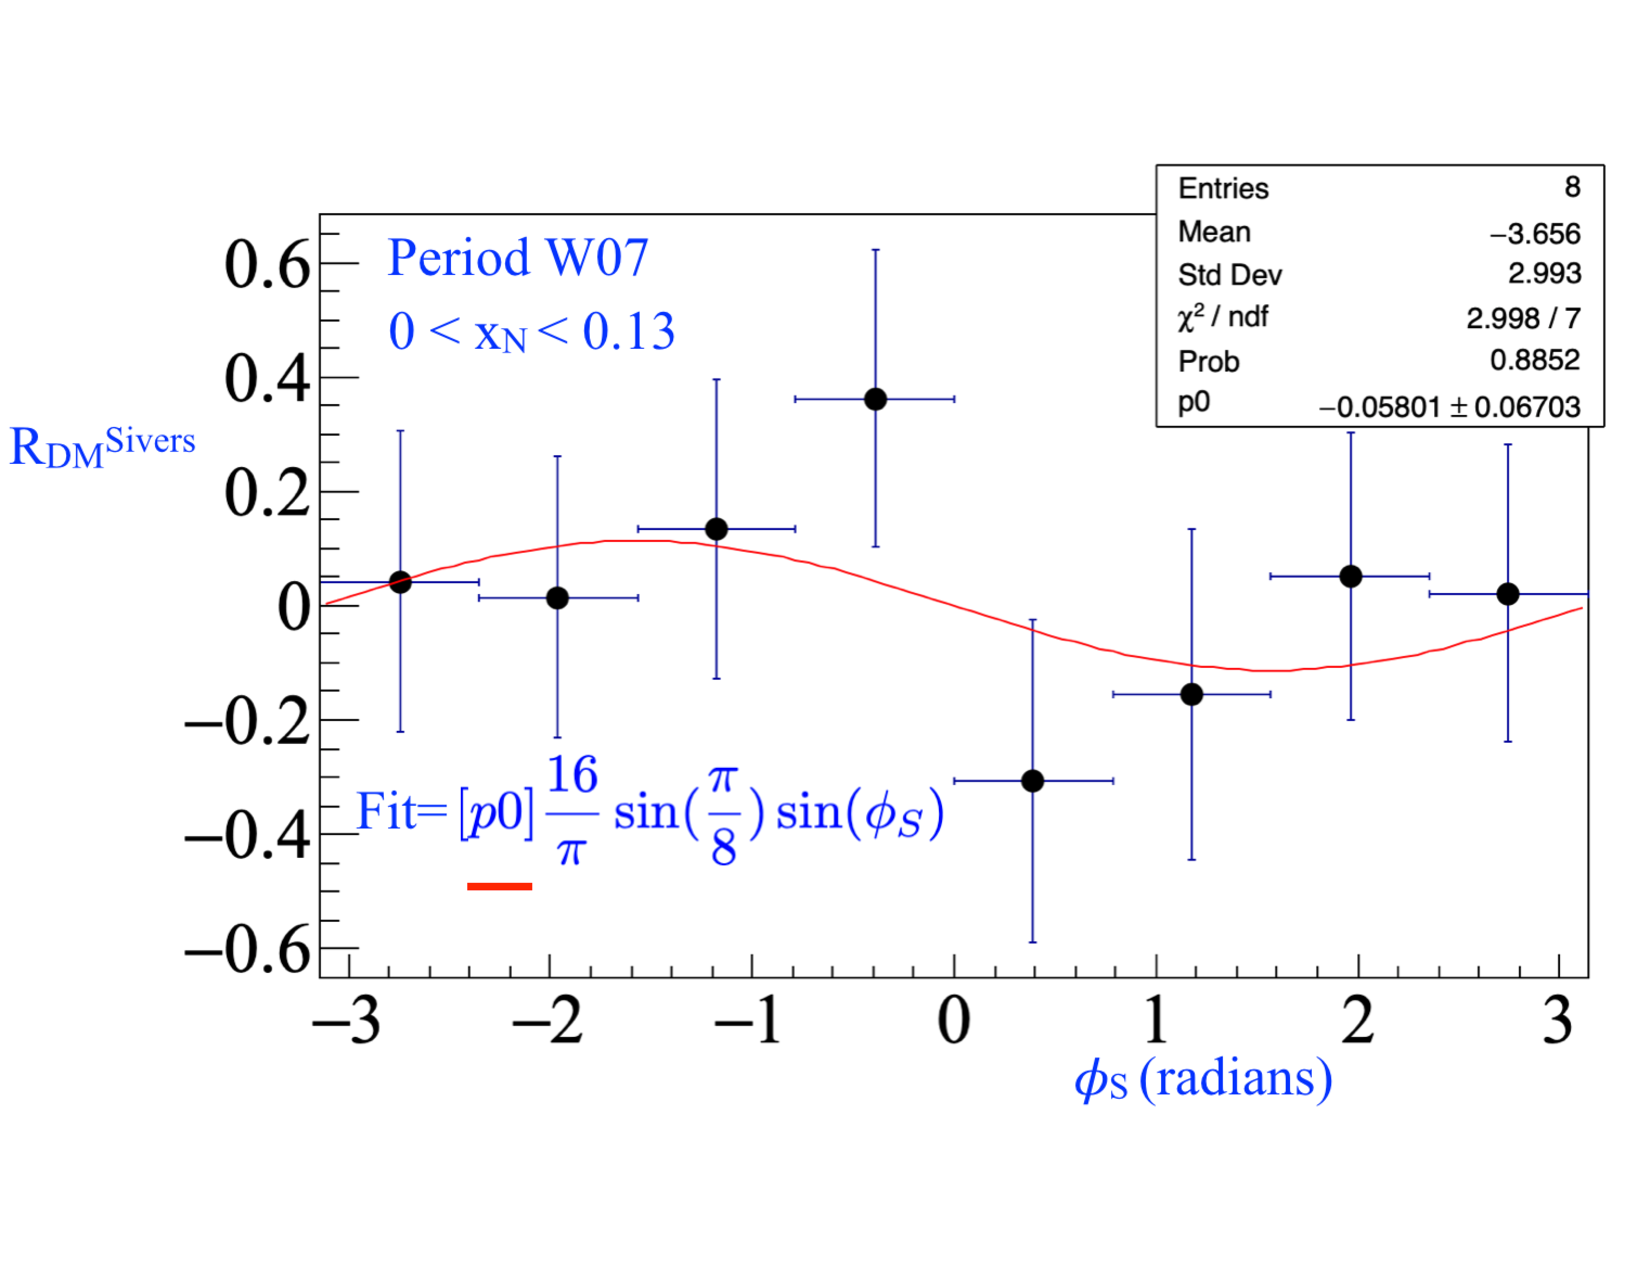
\includegraphics[width=0.6\textwidth, trim=0cm 2.5cm 0cm
    2.5cm,clip]{DRFitSiv}
  \caption{The double ratio as a function of $\phi_S$ used to determine the
    Sivers asymmetry amplitude.  This is for period W07 and the lowest bin in
    $x_N$.  The red line shows the fit.  The results of the fit are shown in the
    statistics box.}
  \label{fig::DRFitSiv}
\end{figure}

\subsection{Results}
As explained in Sec~\ref{sec::doubleratio_results}, the asymmetry amplitudes are
determined for each period and the final asymmetry is determined as a period
weighted average as in Eq.~\ref{equ::wAvg}.  For the same reason as the previous
analyses and explained in Sec~\ref{sec::doubleratio_results}, the polarization
and virtual photon depolarization factors from each period are used to correct
the asymmetry amplitude determined in each period.  The final results are shown
in Fig.~\ref{fig::wA_results} along with the results from the release values.
As can be seen the results agree with those results obtained for the release
which was a requirement before the results could be released to the
public~\cite{Matousek:2018qqd}.

\begin{figure}[h!t]
  \centering 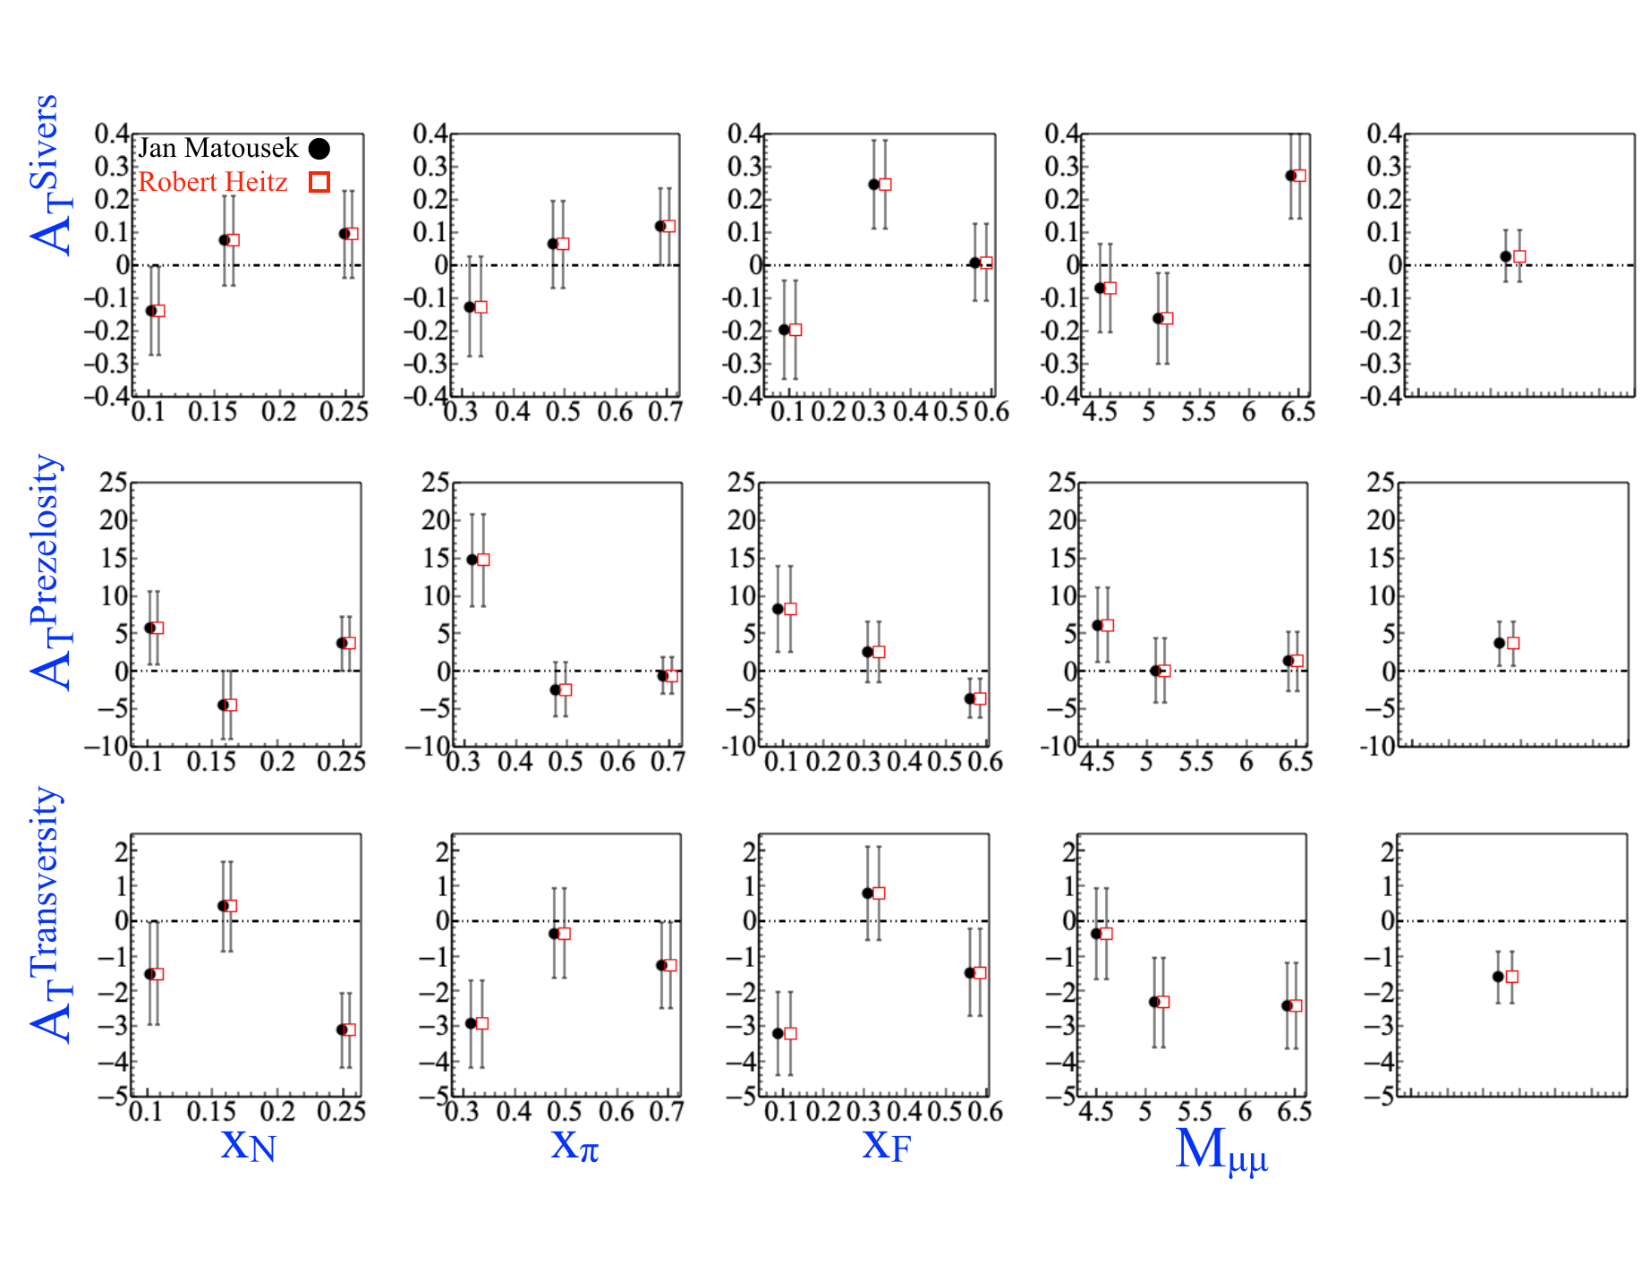
\includegraphics[width=\textwidth,trim=0.2cm 1.5cm 0.2cm 1.5cm,
    clip]{wA_results}
  \caption{The comparison of weighted asymmetry amplitude results from the
    released values from Jan Matousek (black) and the cross checker Robert Heitz
    (red).  From the top row down the asymmetry amplitudes are
    $A_T^{\sin(\phi_S) q_T/M_N}$, $A_T^{\sin(2\phi+\phi_S)
      q^3_T/(2M_{\pi}M_N^2)}$ and $A_T^{\sin(2\phi-\phi_S) q_T/M_{\pi}}$
    respectively.}
  \label{fig::wA_results}
\end{figure}


\section{Left-Right Asymmetries} \label{sec::leftrightasym}

This section goes over the analysis details for measuring the left-right
asymmetry from the transversely polarized Drell-Yan data.  A theoretical
introduction showing how the left-right asymmetry is related to the Sivers TMD
PDF and related past results for this asymmetry are given in
Sec~\ref{sec::lr_theory}.  In short the measured asymmetry can be defined as
\begin{equation}
  A_{lr} = \frac{1}{|S_T|}
  \frac{\sigma_l - \sigma_r}{\sigma_l +
    \sigma_r},
\end{equation}
\noindent
which when assuming the leading order Drell-Yan cross-section,
Eq.~\ref{equ::DY_MostusefulXsect}, is related to the Sivers asymmetry amplitude
as
\begin{equation}
  A_{lr} = \frac{2A_T^{\sin(\phi_S)}}{\pi}.
\end{equation}

There are many ways to determine the left-right asymmetry.  The relevant
techniques for the 2015 COMPASS setup are described and compared to ensure
confidence of the end results.  

\subsection{Asymmetry Extractions}
\subsubsection{Geometric Mean} \label{sec::GeoMean}
The most basic method to determine the left-right asymmetry is

\begin{equation}
  \label{equ::simpleAN}
  A_{lr,simple} = \frac{1}{|S_T|}
    \frac{N_l - N_r}{N_l + N_r},
\end{equation}

\noindent
where $N_l = \int_{\phi_S=0}^{\phi_S=\pi}N(\phi_S)d\phi_S$ denotes the counts
measured left and $N_r = \int_{\phi_S=\pi}^{\phi_S=2\pi}N(\phi_S)d\phi_S$
denotes the counts measured right.  Eq.~\ref{equ::simpleAN} can be used to
determine the left-right asymmetry per target cell.  An intuitive picture of
left and right defined in the target frame is shown in
Fig.~\ref{fig::leftright}.  This simple method to determine the left-right
asymmetry is intuitive and can be helpful for visualizing the forthcoming
methods to determine $A_{lr}$.  Left and right in all definitions in this
section are determined relative to the target spin direction as

\begin{equation}
  \label{equ::Defleftright}
  \begin{aligned}
    &\text{Left}: \hat{q}_T \cdot (\hat{S}_T \times \hat{P}_{\pi}) > 0 \\
    &\text{Right}: \hat{q}_T \cdot (\hat{S}_T \times \hat{P}_{\pi}) < 0, 
  \end{aligned}
\end{equation}

\noindent
where $\hat{q}_T$, $\hat{S}_T$ and $\hat{P}_{\pi}$ are unit vectors in the
target reference frame for the virtual photon transverse momentum, the target
spin and the beam pion momentum respectively.

\begin{figure}[h!t]
  \centering
  \includegraphics[width=0.6\textwidth, trim=7cm 6cm 7cm 7cm,clip]{leftright}
  \caption{The definition of the left plane (red) and right plane (green)
    defined from a target spin up configuration in the target frame}
  \label{fig::leftright}
\end{figure}

The simple definition of the left-right asymmetry, Eq.~\ref{equ::simpleAN}, is
unfortunately dependent on the spectrometer acceptance.  This is can be realized
from the fact that the definition of the detected counts,
Eq.~\ref{equ::countsdef}, depends on the spectrometer acceptance $a(\phi_S)$
which therefore means $A_{lr,simple}$ also depends on the spectrometer
acceptance.  This is a problem because the spectrometer acceptance can change
with time and space and therefore can be dependent on the physical kinematics
which produced the event.  Such dependencies can cause unphysical false
asymmetries in the measurement of $A_{lr}$ and must therefore be removed or must
be included as systematic effects. \par

Forming the geometric mean asymmetry is a way to determine the left-right
asymmetry without acceptance effects from the spectrometer.  The geometric mean
asymmetry is defined as
\begin{equation}
  \label{equ::ANgeomean}
  A_{lr,geo} =
  \frac{1}{|S_T|}
  \frac{\sqrt{N_l^{\uparrow}N_r^{\downarrow}}
    - \sqrt{N_r^{\uparrow}N_r^{\downarrow}}
  }{
    \sqrt{N_l^{\uparrow}N_l^{\downarrow}}
    + \sqrt{N_r^{\uparrow}N_r^{\downarrow}} },
\end{equation}

\noindent
which also defines a left-right asymmetry per target cell.  It is not difficult
to simplify the geometric mean asymmetry as
\begin{equation}
  \label{equ::ANgeomean_expand}
  A_{lr,geo} = \frac{1}{|S_T|}\frac{\kappa_{geo}
    \sqrt{\sigma_l\sigma_l} -
    \sqrt{\sigma_r\sigma_r}}{\kappa_{geo}
    \sqrt{\sigma_l\sigma_l} + \sqrt{\sigma_r\sigma_r}}
  = \frac{1}{|S_T|}\frac{\kappa_{geo}\sigma_l - \sigma_r}{
    \kappa_{geo}\sigma_l + \sigma_r},
\end{equation}

\noindent
where $\kappa_{geo}$ is a ratio of acceptances defined for the geometric mean as
\begin{equation}
  \kappa_{geo} =
  \frac{
    \sqrt{a^\uparrow_J a^\downarrow_S}
    }{
    \sqrt{a^\uparrow_S a^\downarrow_J}
  },
  \label{equ::accGeoMean}
\end{equation}

\noindent
where $J$ stands for the Jura spectrometer side and $S$ stands for Saleve
spectrometer side which are the west and east sides respectively.  The
assumption made for the notation in Eq.~\ref{equ::accGeoMean}, which will be
made throughout this section, is that the target is polarized exactly vertical
in the target frame.  If this assumption violated, the Jura and Saleve
acceptances blend into each other and Eq.~\ref{equ::accGeoMean} is no longer the
correct notation for the acceptance ratio.  The assumption is violated when the
beam particle and the target polarization do not make a right angle in the
laboratory frame, in which case the target will no longer be polarized
vertically in the target frame.  However the target will be assumed to be
vertically polarized in the target frame strictly for ease of notation.

Relation~\ref{equ::ANgeomean_expand} is equal to $A_{lr}$ if $\kappa_{geo} = 1$.
However as stated previously, time effects can vary $\kappa_{geo}$ from
unity. These effects are estimated through false asymmetry analysis and included
in the systematic uncertainties described in Sec~\ref{sec::systematics}.
Equation~\ref{equ::ANgeomean} is therefore to a good approximation an acceptance
free method to determine $A_{lr}$.  It is also defined for the upstream and
downstream cells independently and therefore can be used as a consistency check
between the two target cells.

The statistical uncertainty of the geometry mean is
\begin{equation}
  \delta A_{lr,geo} = \frac{1}{|S_T|}
  \frac{
    \sqrt{
      N_{l}^{\uparrow}N_{l}^{\downarrow}
      N_{\mathrm{r}}^{\uparrow}N_{r}^{\downarrow}
    }
  }{
    \Big( \sqrt{N_{l}^{\uparrow}N_{l}^{\downarrow}} +
    \sqrt{N_{r}^{\uparrow}N_{r}^{\downarrow}} \Big)^2
  }
  \sqrt{
    \frac{1}{N_{l}^{\uparrow}} +
    \frac{1}{N_{l}^{\downarrow}} +
    \frac{1}{N_{r}^{\uparrow}} +
    \frac{1}{N_{r}^{\downarrow}}
  } \quad,
\end{equation}

\noindent
which reduces to $\frac{1}{|S_T|}\frac{1}{\sqrt{N}}$, where $N = N^\uparrow_l +
N^\downarrow_l + N^\uparrow_r + N^\downarrow_r$, in the case of equal statistics
per target cell meaning $N^\uparrow_l = N^\downarrow_l = N^\uparrow_r =
N^\downarrow_r = N/4$.

\subsubsection{Two-Target Geometric Mean} \label{sec::TwoTargGeoMean}
The previous geometric mean asymmetry determined an $A_{lr}$ per target cell.
As described in Sec~\ref{sec::datasample} however, COMPASS had two oppositely
polarized target cells in 2015.  It is desirable from a statistical point of
view and for comparison purposes to determine one $A_{lr}$ from the 2015 COMPASS
setup.  This can be accomplished by modifying the geometric mean to add both
target cells as follows:

\begin{equation}
  \label{equ::AN4TargGeomean}
  A_{lr,2Targ} =
  \frac{1}{|S_T|}
  \frac{ \sqrt[4]{ N_{1,l}^\uparrow N_{1, l}^\downarrow
      N_{2,l}^\uparrow N_{2, l}^\downarrow }
    - \sqrt[4]{ N_{1,r}^\uparrow N_{1,r}^\downarrow
      N_{2,r}^\uparrow N_{2,r}^\downarrow }
  }{
    \sqrt[4]{ N_{1,l}^\uparrow N_{1, l}^\downarrow
      N_{2,l}^\uparrow N_{2, l}^\downarrow }
    + \sqrt[4]{ N_{1,r}^\uparrow N_{1,r}^\downarrow
      N_{2,r}^\uparrow N_{2,r}^\downarrow } }.
\end{equation}

As in the basic geometric mean asymmetry, Sec~\ref{sec::GeoMean}, left and right
are determined relative to the spin direction of the target as in
Eq.~\ref{equ::Defleftright}.  Similarly to Eq.~\ref{equ::ANgeomean_expand}, the
two-target geometric mean asymmetry can be written as
\begin{equation}
  A_{lr,2Targ}= \frac{1}{|S_T|}
  \frac{
    \kappa_{2Targ} \sqrt[4]{\sigma_l\sigma_l\sigma_l\sigma_l} -
    \sqrt[4]{\sigma_r\sigma_r\sigma_r\sigma_r}
  }{
    \kappa_{2Targ} \sqrt[4]{\sigma_l\sigma_l\sigma_l\sigma_l} +
    \sqrt[4]{\sigma_r\sigma_r\sigma_r\sigma_r}
  }
  =
  \frac{1}{|S_T|}
  \frac{\kappa_{2Targ}\sigma_l - \sigma_r}{
    \kappa_{2Targ}\sigma_l + \sigma_r},
  \label{equ::AN2targAcceptCancel}
\end{equation},

\noindent
where now $\kappa_{2Targ}$ is the ratio of acceptances from all targets and
polarizations.  This inclusive acceptance ratio is defined as
\begin{equation}
  \label{equ::acc4TargGeoMean}
  \kappa_{2Targ} =
  \frac{
    \sqrt[4]{
      a^\uparrow_{1,J}
      a^\downarrow_{1,S}
      a^\uparrow_{2,J}
      a^\downarrow_{2,S}}
  }{
    \sqrt[4]{
      a^\uparrow_{1,S}
      a^\downarrow_{1,J}
      a^\uparrow_{2,S}
      a^\downarrow_{2,J}}
  }.
\end{equation}

\noindent
In this case the acceptance ratio is expected to vary less with time and
therefore be closer to unity than the normal geometric mean acceptance ratio,
Eq.~\ref{equ::accGeoMean}.  This is a consequence of having the different target
cells oppositely polarized.  Rewriting Eq.~\ref{equ::acc4TargGeoMean} with
sub-period superscripts instead of target polarization superscripts results in
the relation

\begin{equation}
  \label{equ::acc4TargGeoMean_subperiod}
  \kappa_{2Targ} =
  \frac{ \sqrt[4]{ a^{one}_{1,J} a^{two}_{1,S} a^{two}_{2,J} a^{one}_{2,S} }
  }{
    \sqrt[4]{ a^{one}_{1,S} a^{two}_{1,J} a^{two}_{2,S} a^{one}_{2,J} }
  }
\end{equation}

\noindent
where sub-period $one$ is with the upstream target polarized up and the
downstream target polarized down and vise versa for sub-period $two$.  From
Eq.~\ref{equ::acc4TargGeoMean_subperiod} it is more evident that the acceptance
ratio terms for sub-period $two$ are reciprocal to the terms for sub-period
$one$ and therefore the acceptance ratio is expected to be more stably close to
unity.

Finally the statistical uncertainty of the two target geometric mean is
\begin{equation}
  \delta A_{lr,2Targ} = \frac{1}{|S_T|}
  \frac{LR}{\Big( L+R \Big)^2}
  \sqrt{
    \sum_{c,p}
    \Big(
    \frac{1}{N_{c,l}^{p}}
    + \frac{1}{N_{c,r}^p}
    \Big)
  } \quad,
\end{equation}

\noindent
where $L$ can be thought of as the left counts and equals to
$\sqrt[4]{N_{1,l}^\uparrow N_{1,l}^\downarrow N_{2,l}^\uparrow
  N_{2,l}^\downarrow}$ and $R$ can be thought of as the right counts and equals
$\sqrt[4]{N_{1,r}^\uparrow N_{1,r}^\downarrow N_{2,r}^\uparrow
  N_{2,r}^\downarrow}$.  As with the geometric mean asymmetry, in the case of
equal statistic populations in each direction and target polarization, the
statistical uncertainty for the two-target geometric mean also reduces to
$\frac{1}{|S_T|}\frac{1}{\sqrt{N}}$, where $N$ is the sum of all counts.


\subsection{Systematic Studies} \label{sec::systematics}
Several tests were performed to estimate the systematic uncertainty of the
left-right asymmetry.  The systematic uncertainties are determined by adding all
non-zero systematic uncertainties in quadrature.  The impact from each source of
systematic error is summarized in Table.~\ref{tab::sysError}.

\subsubsection{Period Compatibility (Time Dependence)}\label{sec::sysPulls}
The asymmetries calculated for each time period in each kinematic bin are shown
in Fig.~\ref{fig::allPhysBinned4Targ}.

\begin{figure}[h!t]
  \begin{center}
    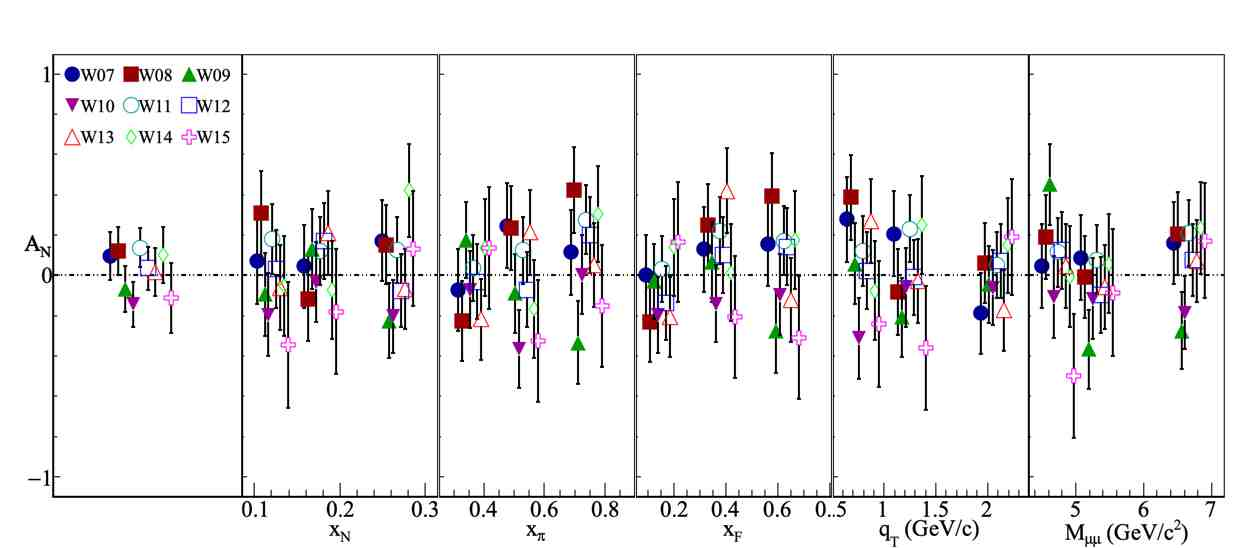
\includegraphics[width=\textwidth,trim=0cm 5cm 0cm
      5cm,clip]{allPhysBinned4Targ}
    \caption{$A_{lr}$ determined for each period}
    \label{fig::allPhysBinned4Targ}
  \end{center}
\end{figure}

\noindent
By eye the asymmetry fluctuations appear to be statistically compatible.  To
quantify the compatibility of the asymmetries between the periods, a pull
distribution is formed where the pull value is defined as

\begin{equation}
  \label{eq::pull}
  \Delta\mathrm{A}_i =
  \frac{
    \mathrm{A}_i - \langle \mathrm{A} \rangle
  }{
    \sqrt{
      \sigma^2_{\mathrm{A}_i} - \sigma^2_{\langle \mathrm{A} \rangle}
    }
  },
\end{equation}

\noindent
and is determined for each period and kinematic bin.  There are therefore 3
(number of bins) x 5 (number of kinematics) x 9 (number of periods) = 135
entries in the pull distribution. The pull distribution is shown in
Fig.~\ref{fig::pull4Targ} along with a Gaussian fit to determine the
distributions width and average.  If the asymmetries all come from the same
parent distribution then, due to the central limit theorem, the pull
distribution will be a Gaussian distribution with zero mean and unit variance.
The discrepancy of the pull distribution from a standard Gaussian distribution
is used to determine a systematic error as

\begin{equation}
  \label{equ::sysErrorPull}
  \frac{\sigma_{\mathrm{systematic}}}{\sigma_{\mathrm{statistical}}} =
  \sqrt{|\sigma^2_{\mathrm{pull}} - 1|} + \frac{\mu_{\mathrm{pull}}}{2}.
\end{equation}

\begin{figure}[h!t]
  \begin{center}
    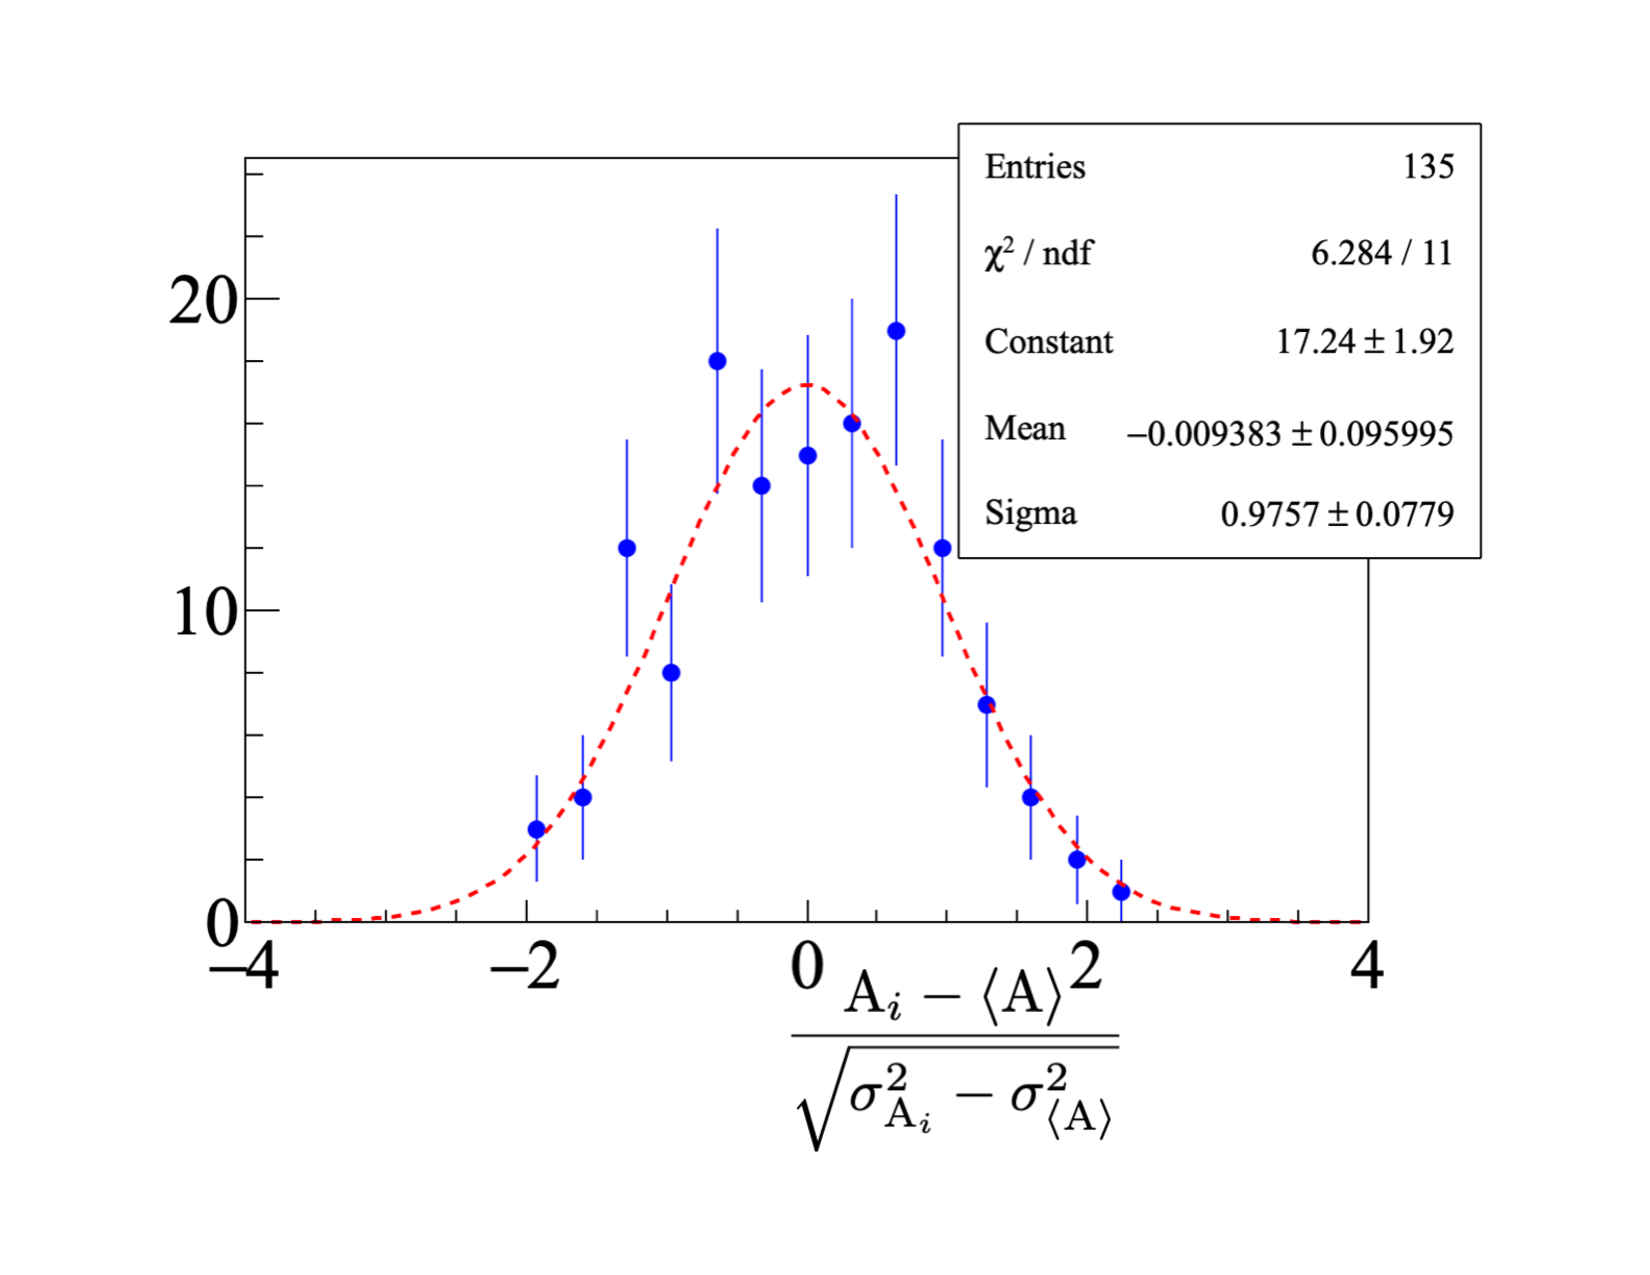
\includegraphics[width=0.6\textwidth, trim=2cm 2cm 2cm 2cm,clip]{pull4Targ}
    \caption{Pull distribution from the two-target geometric mean}
    \label{fig::pull4Targ}
  \end{center}
\end{figure}

\noindent
As the asymmetries in different kinematic bins are formed using the same data
set, the asymmetries between kinematic binnings are correlated.  For this reason
an uncorrelated pull distribution is also formed for each kinematic bin and also
compared with a standard Gaussian distribution.  These distributions are shown
in Fig.~\ref{fig::allPhysPulls4Targ_fit} along with the results of their
respective Gaussian fits.  For these uncorrelated pull distributions there are
now only 3 (number of bins) x 9(number of periods) = 27 entries in each
kinetically binned pull distributions and only 9 (number of periods) bins in the
integrated pull distribution.

\begin{figure}[h!t]
  \begin{center}
    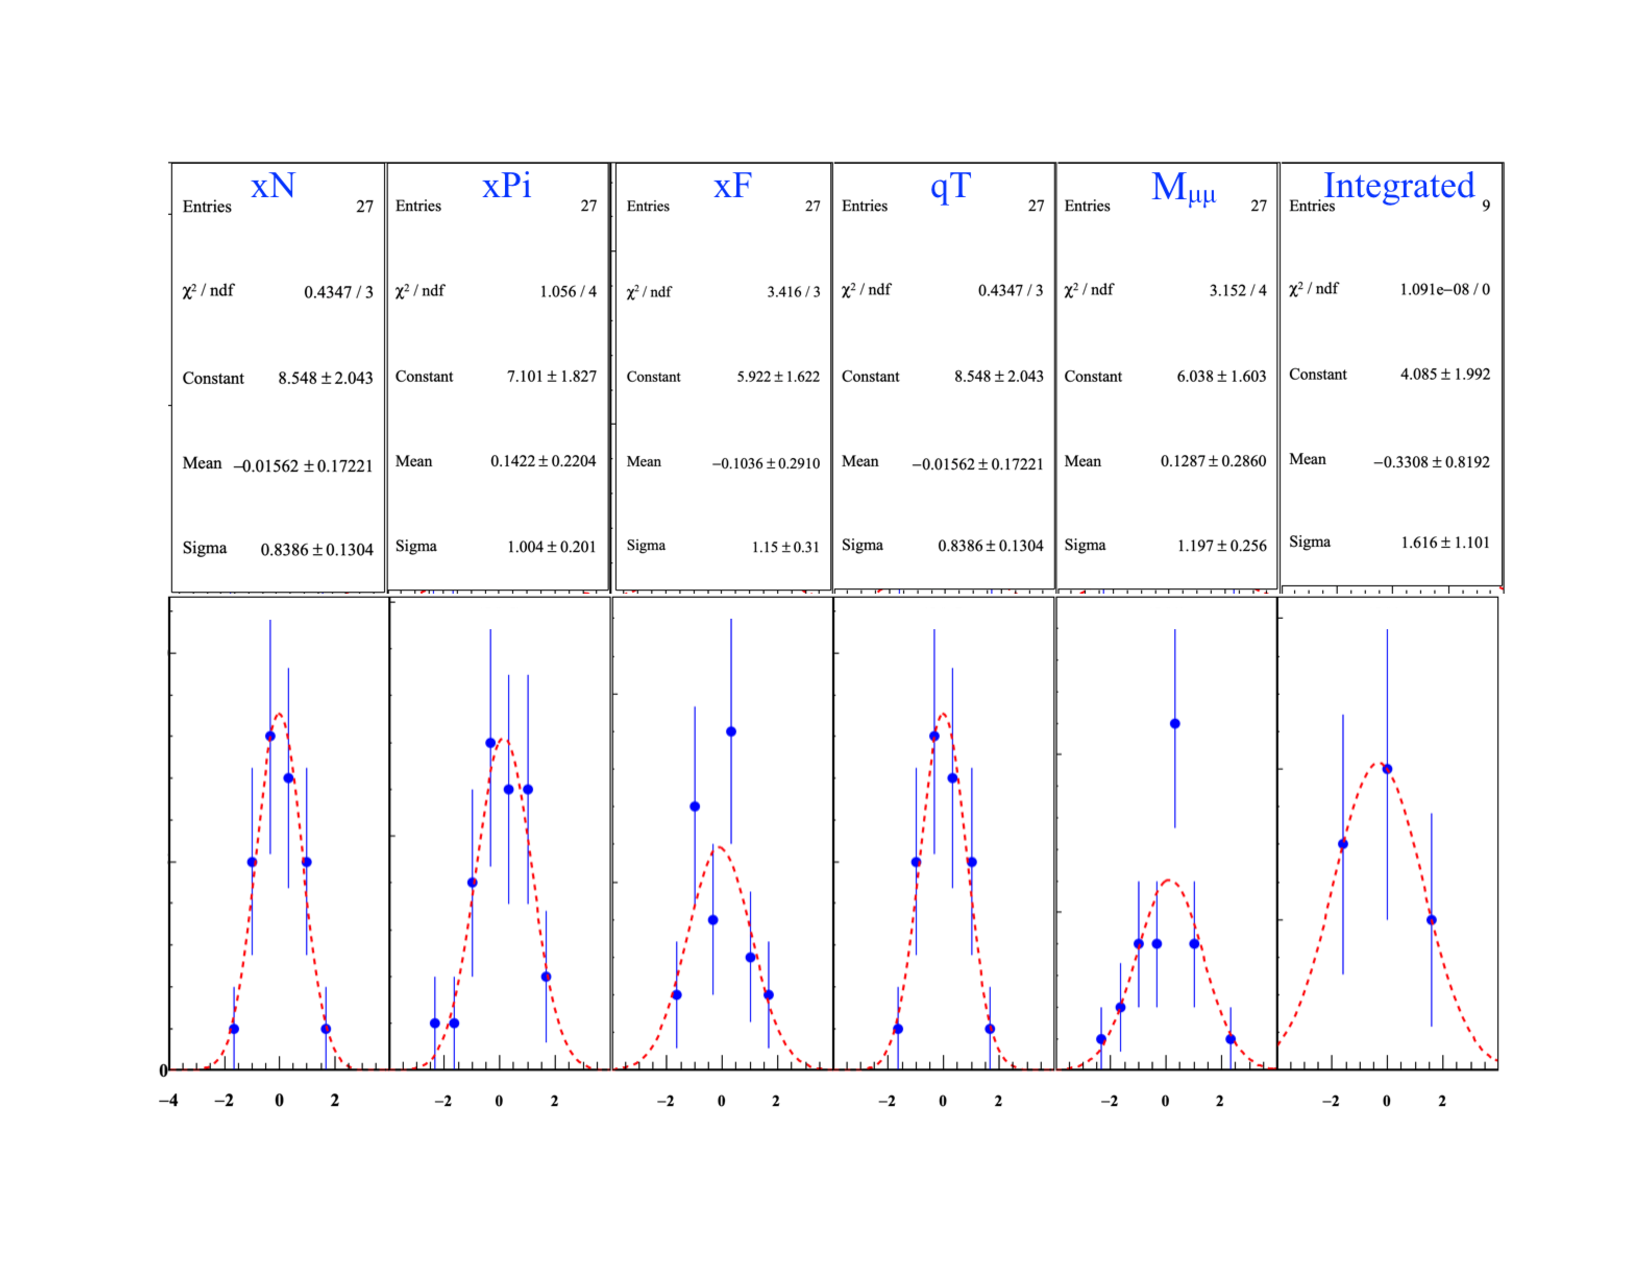
\includegraphics[width=\textwidth, trim=2.5cm 2.5cm 2.5cm 2.5cm,
      clip]{allPhysPulls4Targ_fit}
    \caption{Uncorrelated pull distributions and Results of the Gaussian fit for
      the pull distributions}
    \label{fig::allPhysPulls4Targ_fit}
  \end{center}
\end{figure}

Even though the Gaussian fits did not give exactly a standard Gaussian, the fit
parameters are well compatible with a standard Gaussian within the errors of the
fit.  Therefore no systematic error was assigned due to incompatibility of the
periods.

\subsubsection{Left/Right Event Migration} \label{sec::syslrEventMigration}
The spectrometer has finite resolution for any measured quantity.  For this
reason events measured as left outgoing could really be events that are right
outgoing and vise versa.  This left-right misidentification has the result of
diluting spin-dependent effects by effectively having a sample from an
unpolarized target along with the sample from the polarized target.  Therefore
the asymmetry $A_{lr}$ reduces from left-right misidentification and this
effect is included as a systematic effect. 

A Monte-Carlo data set was analyzed to determine the left-right
misidentification percentage.  Four Monte-Carlo processes were generated
corresponding to three background processes and a spin-independent signal
process.  The generator used was PYTHIA8 and the data was generated and
reconstruction at Blue Waters.  The background processes simulated were JPsi
production, Psi' production and open charm (OC) production.  Each of these
backgrounds can decay into two final state muons which results in a background
contamination to the Drell-Yan signal.  Table~\ref{tab::MCproduction} gives the
parameters used for the Monte-Carlo generated.

\begin{table}[h!t]
  \centering
  \caption{Monte-Carlo settings produced on Blue Waters}
  \label{tab::MCproduction}
  \begin{tabular}{ |c|c| }
    \hline
    \textbf{Description}& \textbf{Monte-Carlo Setting Setting} \\ \hline
    \hline
    Event generator& PYTHIA8\\
    \hline

    Pion PDF& GRVPI1\\
    \hline

    Proton PDF& NNPDF23\\
    \hline
    
    Proton/Neutron mixing ratio& 1.96\\
    \hline

    Initial state radiation& on\\
    \hline
    
    Final state radiation& on\\
    \hline
    
    Multiple parton interactions& on\\
    \hline

    GEANT4 detector simulation& TGEANT \\
    \hline

    Simulated detector efficiency distributions& uniform\\
    \hline
    
  \end{tabular}
\end{table}

The generated Monte-Carlo data corresponds to a 4$\pi$ spectrometer acceptance.
The COMPASS spectrometer on the other hand, does not have a full 4$\pi$
acceptance.  Therefore to produce simulated data that corresponds to the actual
data taking conditions, a GEANT4~\cite{AGOSTINELLI2003250} based detector
simulation, called TGEANT~\cite{TGEANTthesis}, simulated the COMPASS
spectrometer response to the generated data.  The data from TGEANT was then
reconstructed with the same reconstruction software as real data.

Misidentification was estimated by comparing the data input to TGEANT with the
output reconstructed data.  The same analysis and cuts were performed on the
simulated and then reconstructed data as were performed on the real data set.
Fig.~\ref{fig::lrMigration} shows the rate of events identified correctly and
incorrectly as a function of $\phi_S$.  Fig.~\ref{fig::lrMigration} is made by
comparing which outgoing direction the generated events emerged with the
outgoing direction the reconstructed events emerged.

\begin{figure}[h!t]
  \centering
  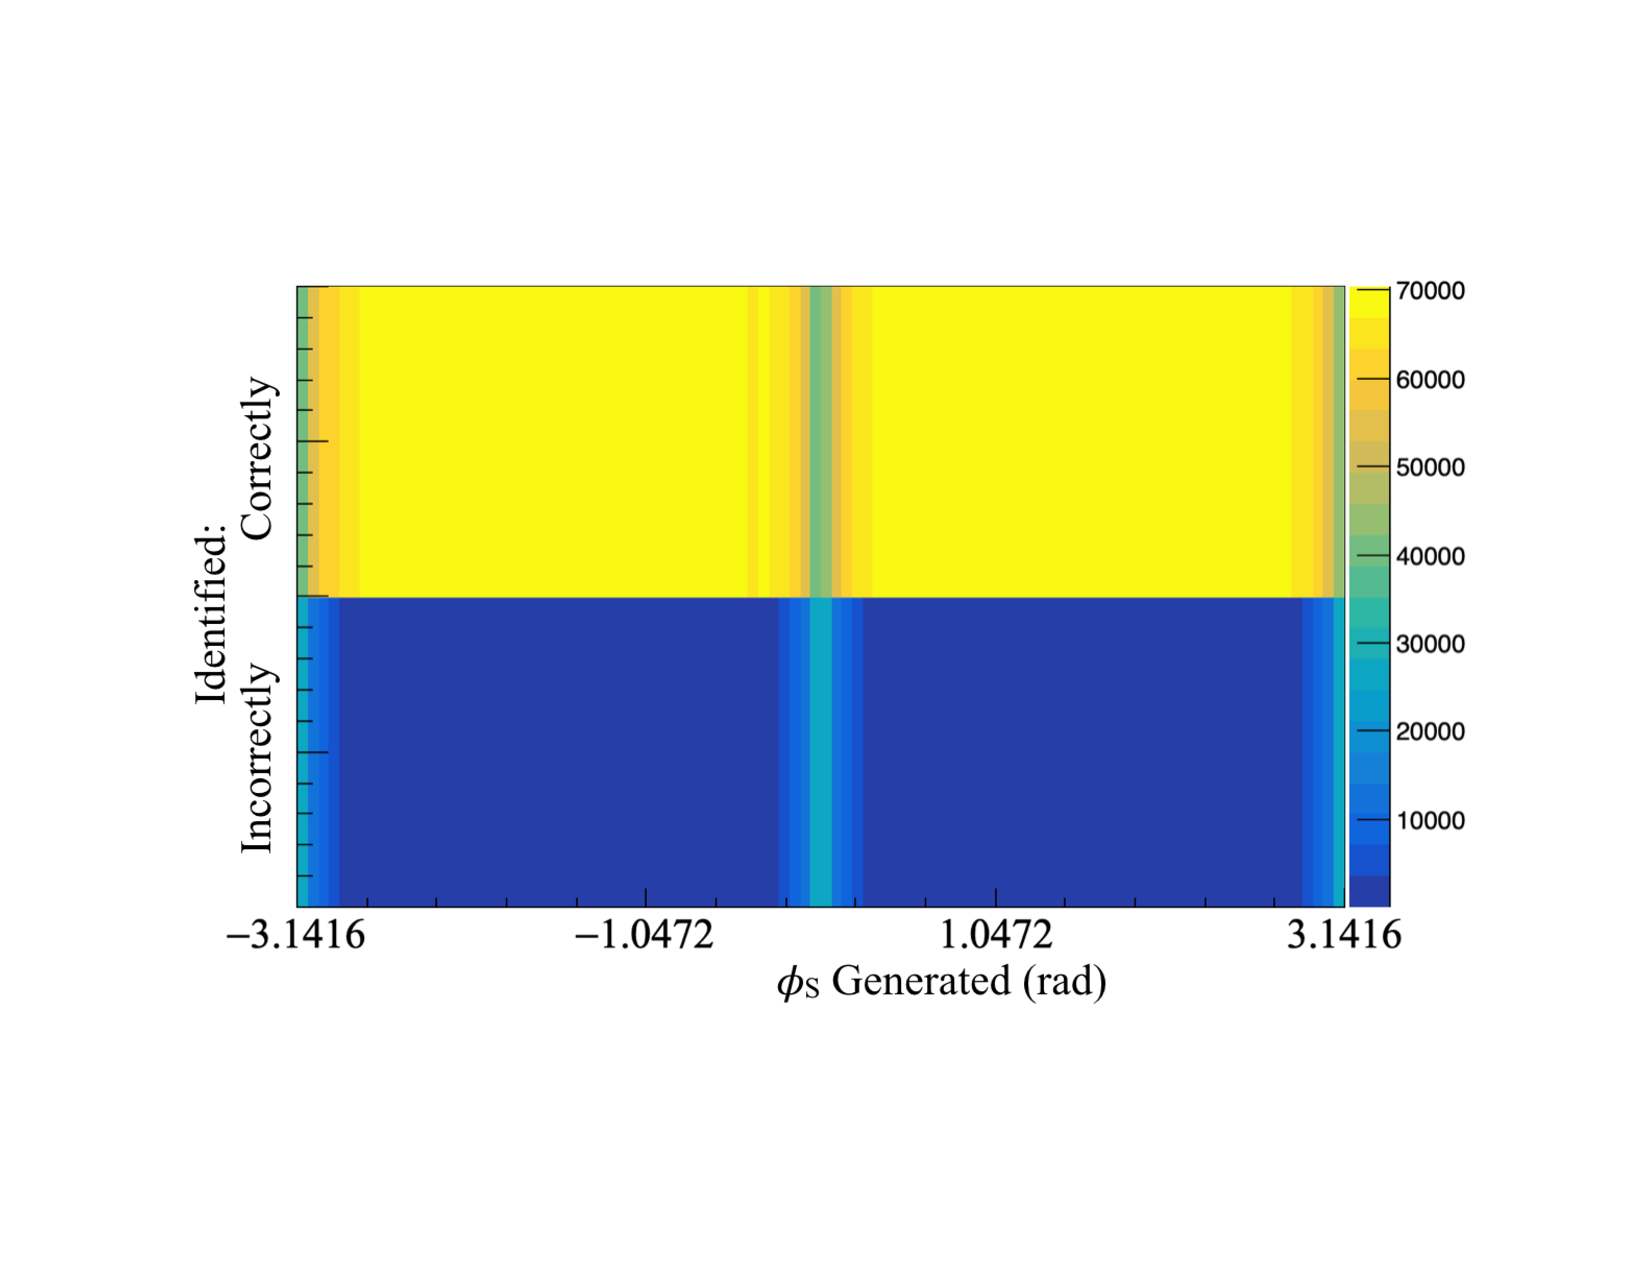
\includegraphics[width=0.6\textwidth,trim=3cm 4cm 3cm 6cm, clip]{lrMigration}
  \caption{The rate of identified correctly and incorrectly left-right events as
    a function of $\phi_{S}$.  This is determined by comparing the generated
    outgoing direction with the reconstructed outgoing direction.  The
    left-right boundary is clearing visible at $\phi_{S}$ = 0~rad and $\phi_{S}$
    = -$\pi$~rad and $\phi_{S}$ = $\pi$~rad}.
  \label{fig::lrMigration}
\end{figure}

\noindent
As is clearly visible in Fig.~\ref{fig::lrMigration}, there is a band of higher
misidentification rate at the border between left and right.  For this reason a
cut on the $\phi_{S}$ variable symmetric about the left-right border was tested
to determine the percent of misidentification as a function of the amount of
$\phi_{S}$ cut.  These results are shown in Fig.~\ref{fig::percentLRmiss}.

\begin{figure}[h!t]
  \centering 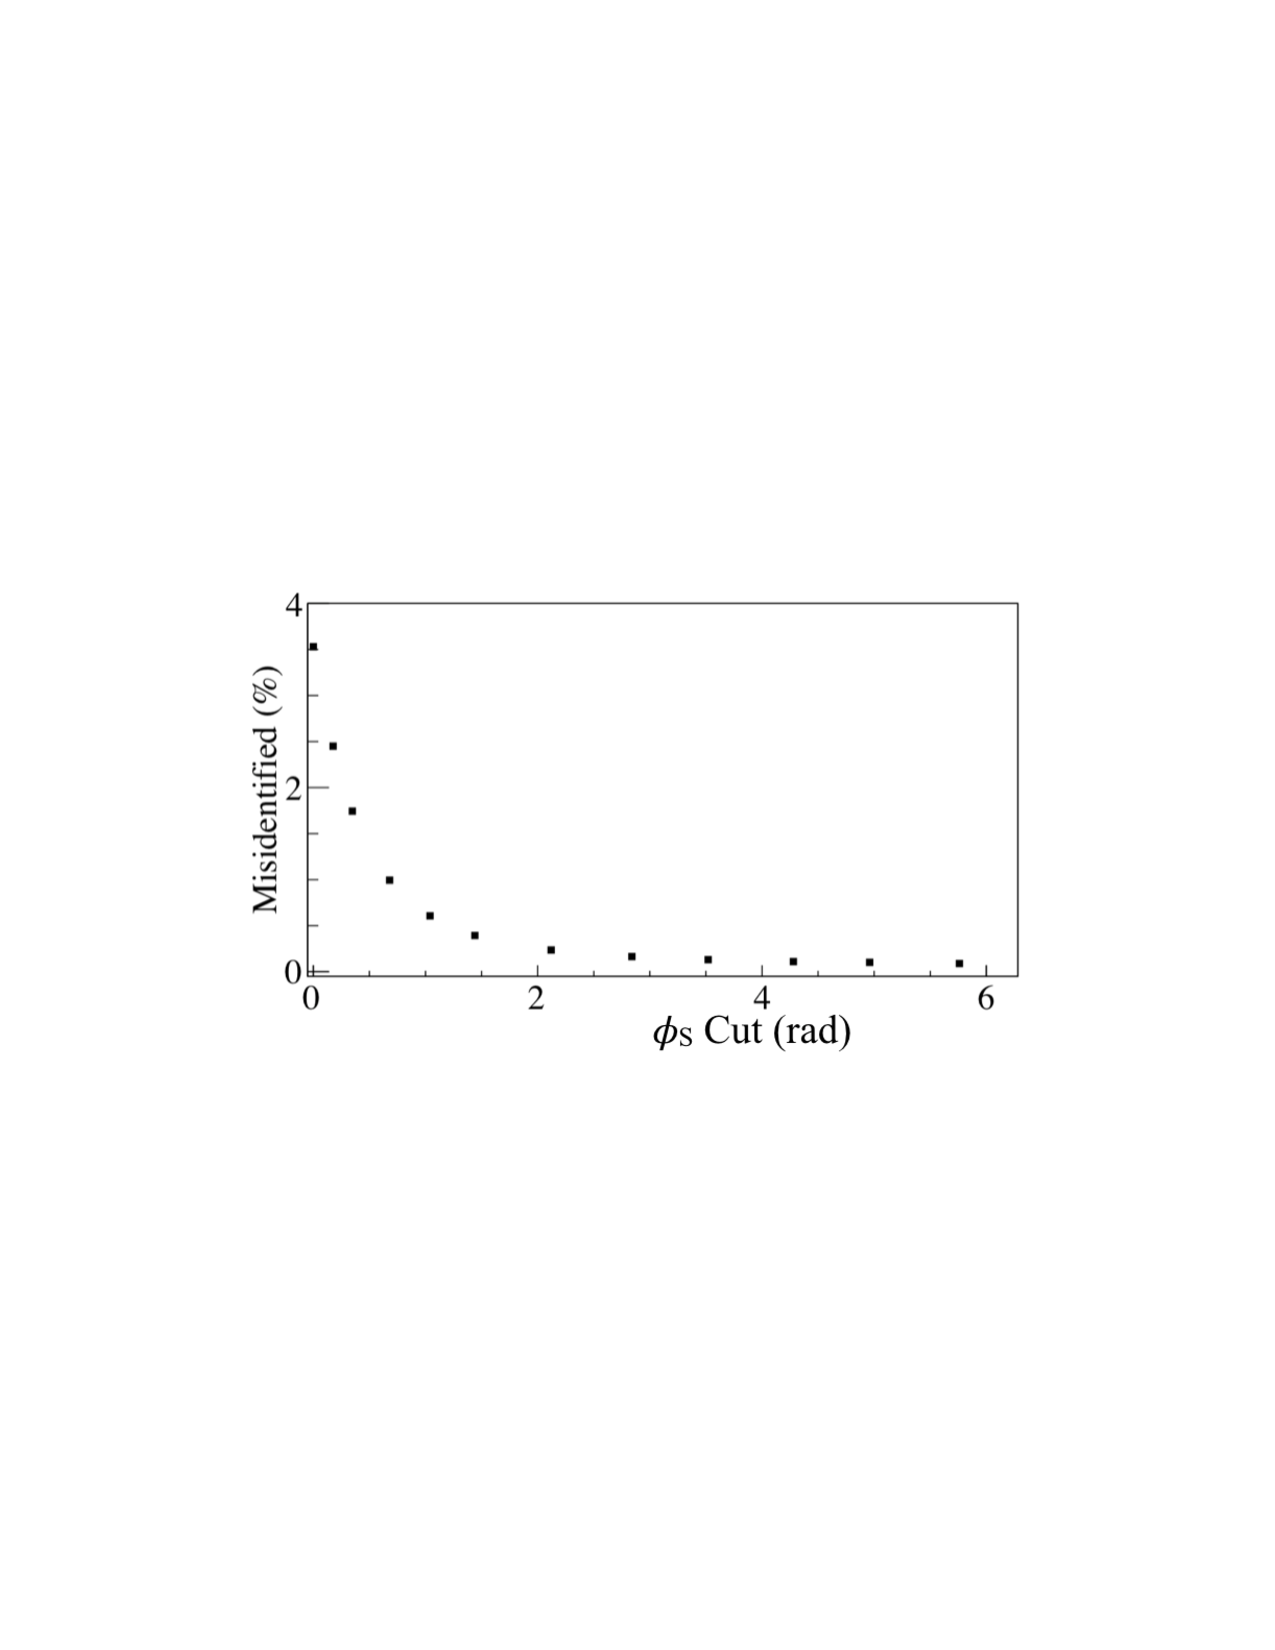
\includegraphics[width=0.5\textwidth, trim=4cm 10cm 4cm 10cm,
    clip]{percentLRmiss}
  \caption{Percent left-right migration as a function of the amount of
    $\phi_{S}$ cut.}
    \label{fig::percentLRmiss}
\end{figure}

The systematic error for left-right migration is calculated as

\begin{equation}
  \delta A_{lr,systematic} = \gamma *A_{lr} + \gamma *\delta A_{lr},
\end{equation}

\noindent
where this expression is derived in Appendix~\ref{app::sysLRmiss}.  No cut on
$\phi_{S}$ was ultimately used for the asymmetry determination.  This is to
avoid loss of statistics and due to the fact that the systematic error is
already small with no cut in $\phi_{S}$.  The integrated systematic error due to
left-right event migration was determined to be 9\% of the statistical error.


\subsubsection{False Asymmetries}
\subsubsection{Acceptance From False Asymmetries}
As was pointed out in Sec.~\ref{sec::GeoMean} and
Sec.~\ref{sec::TwoTargGeoMean}, the asymmetry measurement assumes the acceptance
does not change with time and therefore the acceptance ratio, $\kappa$ is
unitary.  Any deviation from a unitary acceptance ratio is estimated with a
false asymmetry and is taken as a systematic error.  To determine if acceptance
does change with time, a false asymmetry is calculated where the only way the
false asymmetry could be non-zero is if acceptance changes with time.  This
false asymmetry for the two-target geometric mean is

\begin{align}
  \label{equ::falseAcc}
  A_{lr,False} &= 
    \frac{1}{|S_T|}
    \frac{
      \sqrt[4]{
        N_{1,r}^\uparrow N_{1, l}^\downarrow
        N_{2,l}^\uparrow N_{2, r}^\downarrow
      } 
      -\sqrt[4]{
        N_{1,l}^\uparrow N_{1, r}^\downarrow
        N_{2,r}^\uparrow N_{2, l}^\downarrow
      }
    }{
      \sqrt[4]{
        N_{1,r}^\uparrow N_{1, l}^\downarrow
        N_{2,l}^\uparrow N_{2, r}^\downarrow
      } +
      \sqrt[4]{
        N_{1,l}^\uparrow N_{1, r}^\downarrow
        N_{2,r}^\uparrow N_{2, l}^\downarrow
      }
    } \\ \nonumber
    & =
    \frac{1}{|S_T|}
    \frac{
      \alpha_{2Targ} \sqrt[4]{\sigma_r\sigma_l\sigma_l\sigma_r} -
      \sqrt[4]{\sigma_l\sigma_r\sigma_r\sigma_l}
    }{
      \alpha_{2Targ} \sqrt[4]{\sigma_r\sigma_l\sigma_l\sigma_r} +
      \sqrt[4]{\sigma_l\sigma_r\sigma_r\sigma_l}
    }
    = \frac{1}{|S_T|}
    \frac{
      \alpha_{2Targ} - 1     
    }{
      \alpha_{2Targ} + 1
    },
\end{align}

\noindent
where $\alpha_{2Targ}$ is an acceptance ratio and is defined as

\begin{equation} \label{equ::alphaAcc}
  \alpha_{2Targ} =
  \frac{ \sqrt[4]{ a^\uparrow_{1,S}a^\downarrow_{1,S}
      a^\uparrow_{2,J}a^\downarrow_{2,J}}
  }{
    \sqrt[4]{
      a^\uparrow_{1,J} a^\downarrow_{1,J}
      a^\uparrow_{2,S} a^\downarrow_{2,S}
    }
  }.
\end{equation}

\noindent
The false asymmetry, Eq.~\ref{equ::falseAcc}, can be simplified as

\begin{equation}
  A_{lr,False} = 
  \frac{1}{|S_T|}
  \frac{
    \sqrt[4]{ N_{1, S} N_{2, J} }
    - \sqrt[4]{ N_{1, J} N_{2, S} }
  }{
    \sqrt[4]{ N_{1, S} N_{2, J} }
    + \sqrt[4]{ N_{1, J} N_{2, S} }
  }.
\end{equation}

\noindent
That is $A_{lr,False}$ is the normalized difference of counts from each
target cell assuming the upstream target is always polarized down and the
downstream target is always polarized up.  Given that the polarization flips for
both upstream and downstream target cells, $A_{lr,False}$ is an
asymmetry where physical effects cancel out.  The kinematic dependencies of the
false asymmetry are shown in Fig.~\ref{fig::falseAacc} and the kinematic
dependencies of the acceptance ratio, $\alpha_{2Targ}$, are shown in
Fig.~\ref{fig::alpha}.

\begin{figure}[h!t]
  \begin{center}
    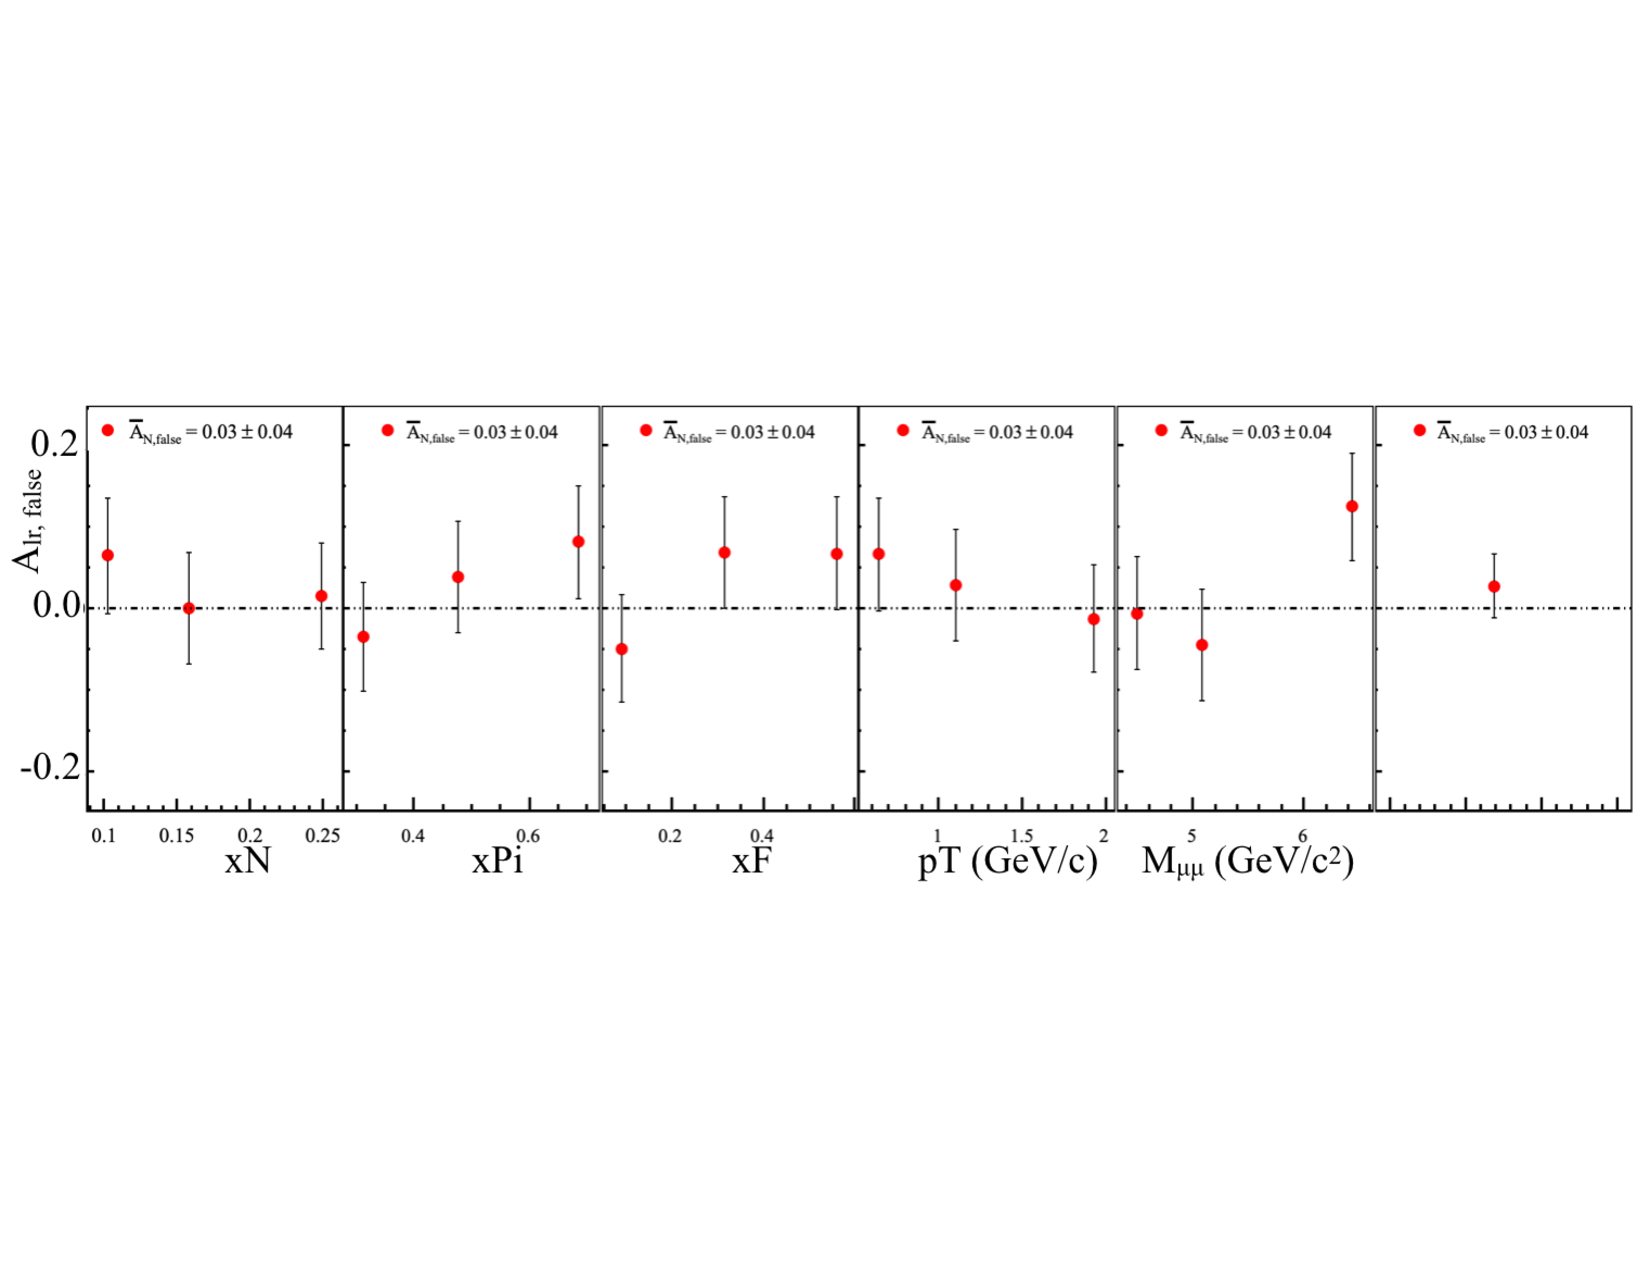
\includegraphics[width=\textwidth, trim=0cm 6.5cm 0cm 6.5cm,
      clip]{falseAacc}
    \caption{False asymmetry, $A_{lr,False}$, to estimate fluctuations in
      acceptance in time}
    \label{fig::falseAacc}
  \end{center}
\end{figure}

\begin{figure}[h!t]
  \begin{center}
    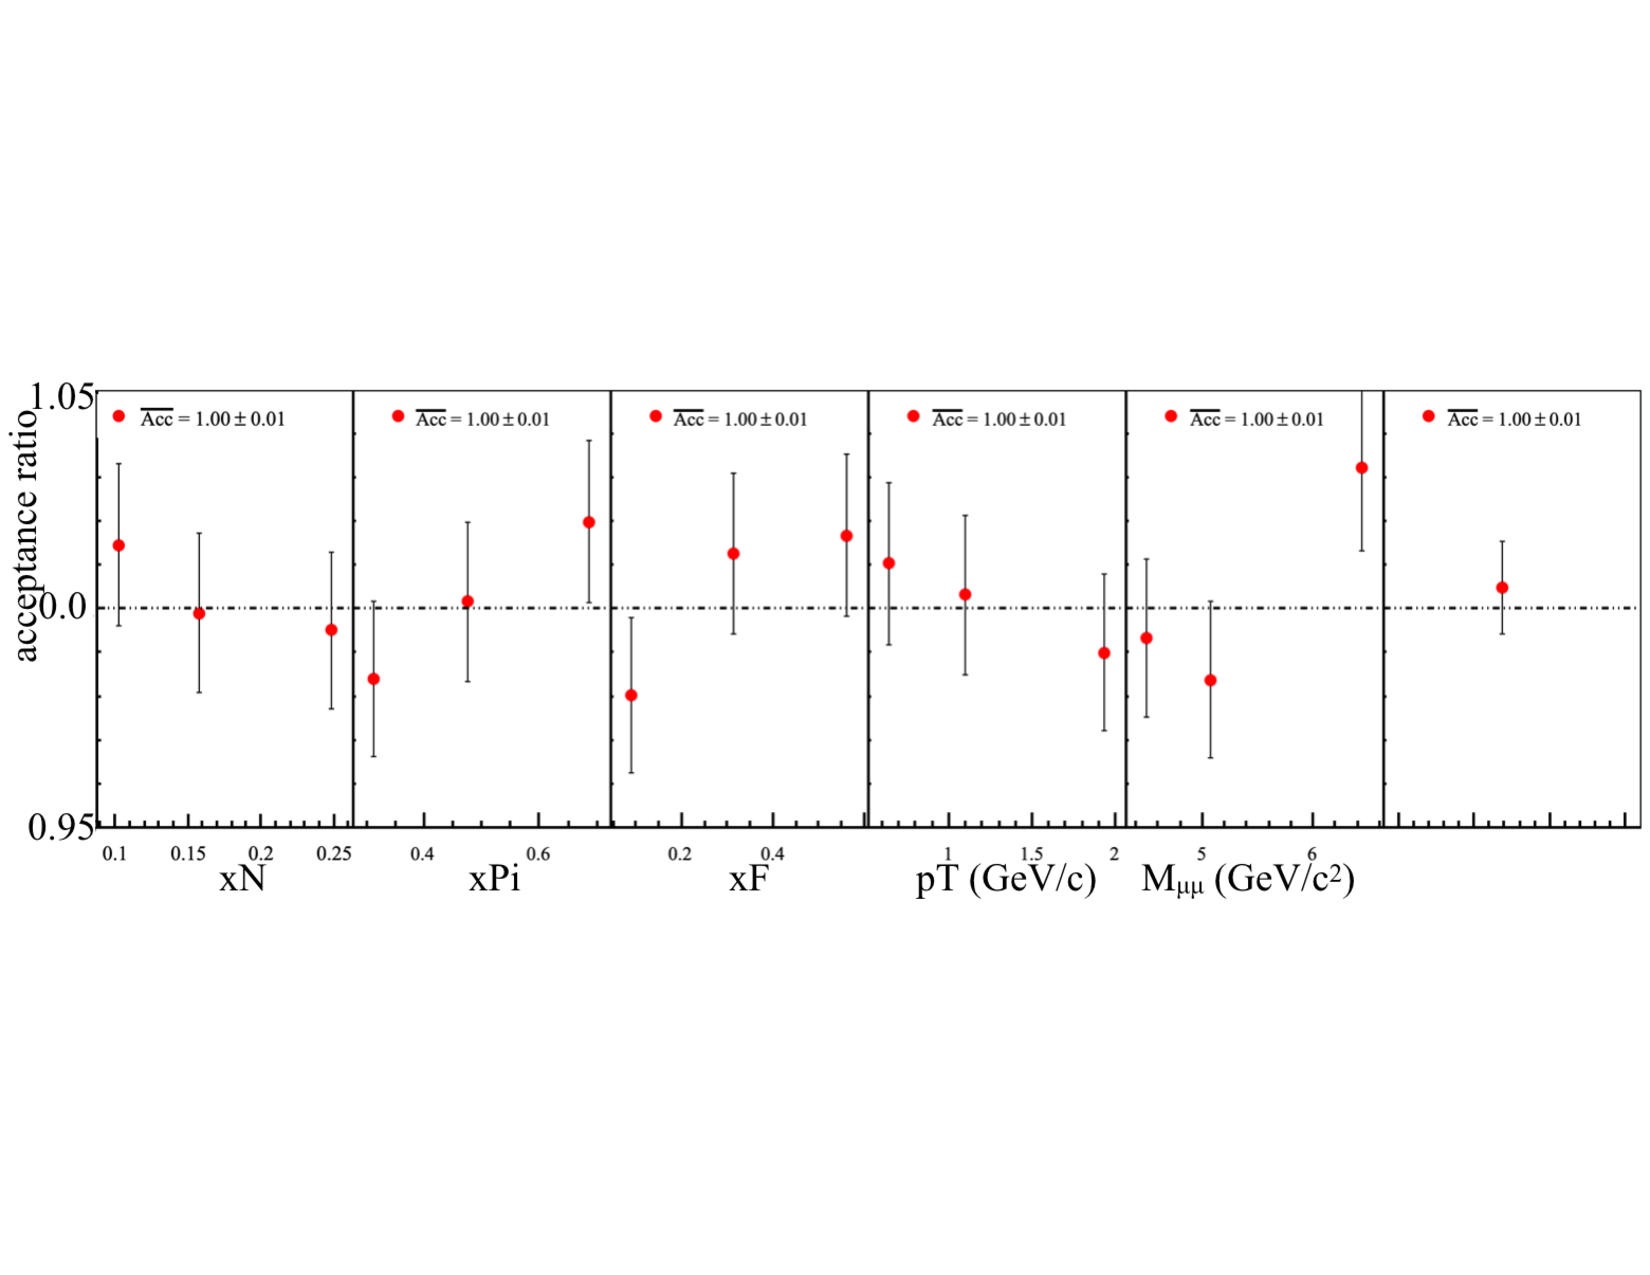
\includegraphics[width=\textwidth, trim=0cm 6cm 0cm 6cm,
      clip]{alpha4Targ}
    \caption{Acceptance ratio $alpha_{2Targ}$, Eq.~\ref{equ::alphaAcc}, used to
      determine the systematic effects from acceptance changes in time}
    \label{fig::alpha}
  \end{center}
\end{figure}

While $\alpha_{2Targ}$ is an acceptance ratio it is not the same as,
$\kappa_{2Targ}$ the acceptance ratio in the true asymmetry.  However
$\alpha_{2Targ}$ is similar to $\kappa_{2Targ}$ in that $\alpha_{2Targ}$ will
only be different from unity as a result of time changes in the spectrometer.
Therefore it is assumed $\alpha_{2Targ}$ can be used as a good estimate of the
true acceptance ratio fluctuations.  The systematic error due to acceptance
fluctuations is determined as

\begin{equation}
  \delta A_{lr,systematic} =
  \frac{1}{|S_T|}
  \Big(\frac{|\alpha_{2Targ}-1|}{2}
  + \delta_{\frac{|\alpha_{2Targ}-1|}{2}} \Big),
\end{equation}

\noindent
where this expression is derived in Appendix~\ref{app::sysAcc}.  The kinematic
dependence of the systematic error normalized to the statistical error is shown
in Fig.~\ref{fig::accSysStat}.  The binned average systematic error due to
acceptance is 20\% of the statistical error.

\begin{figure}[h!t]
  \begin{center}
    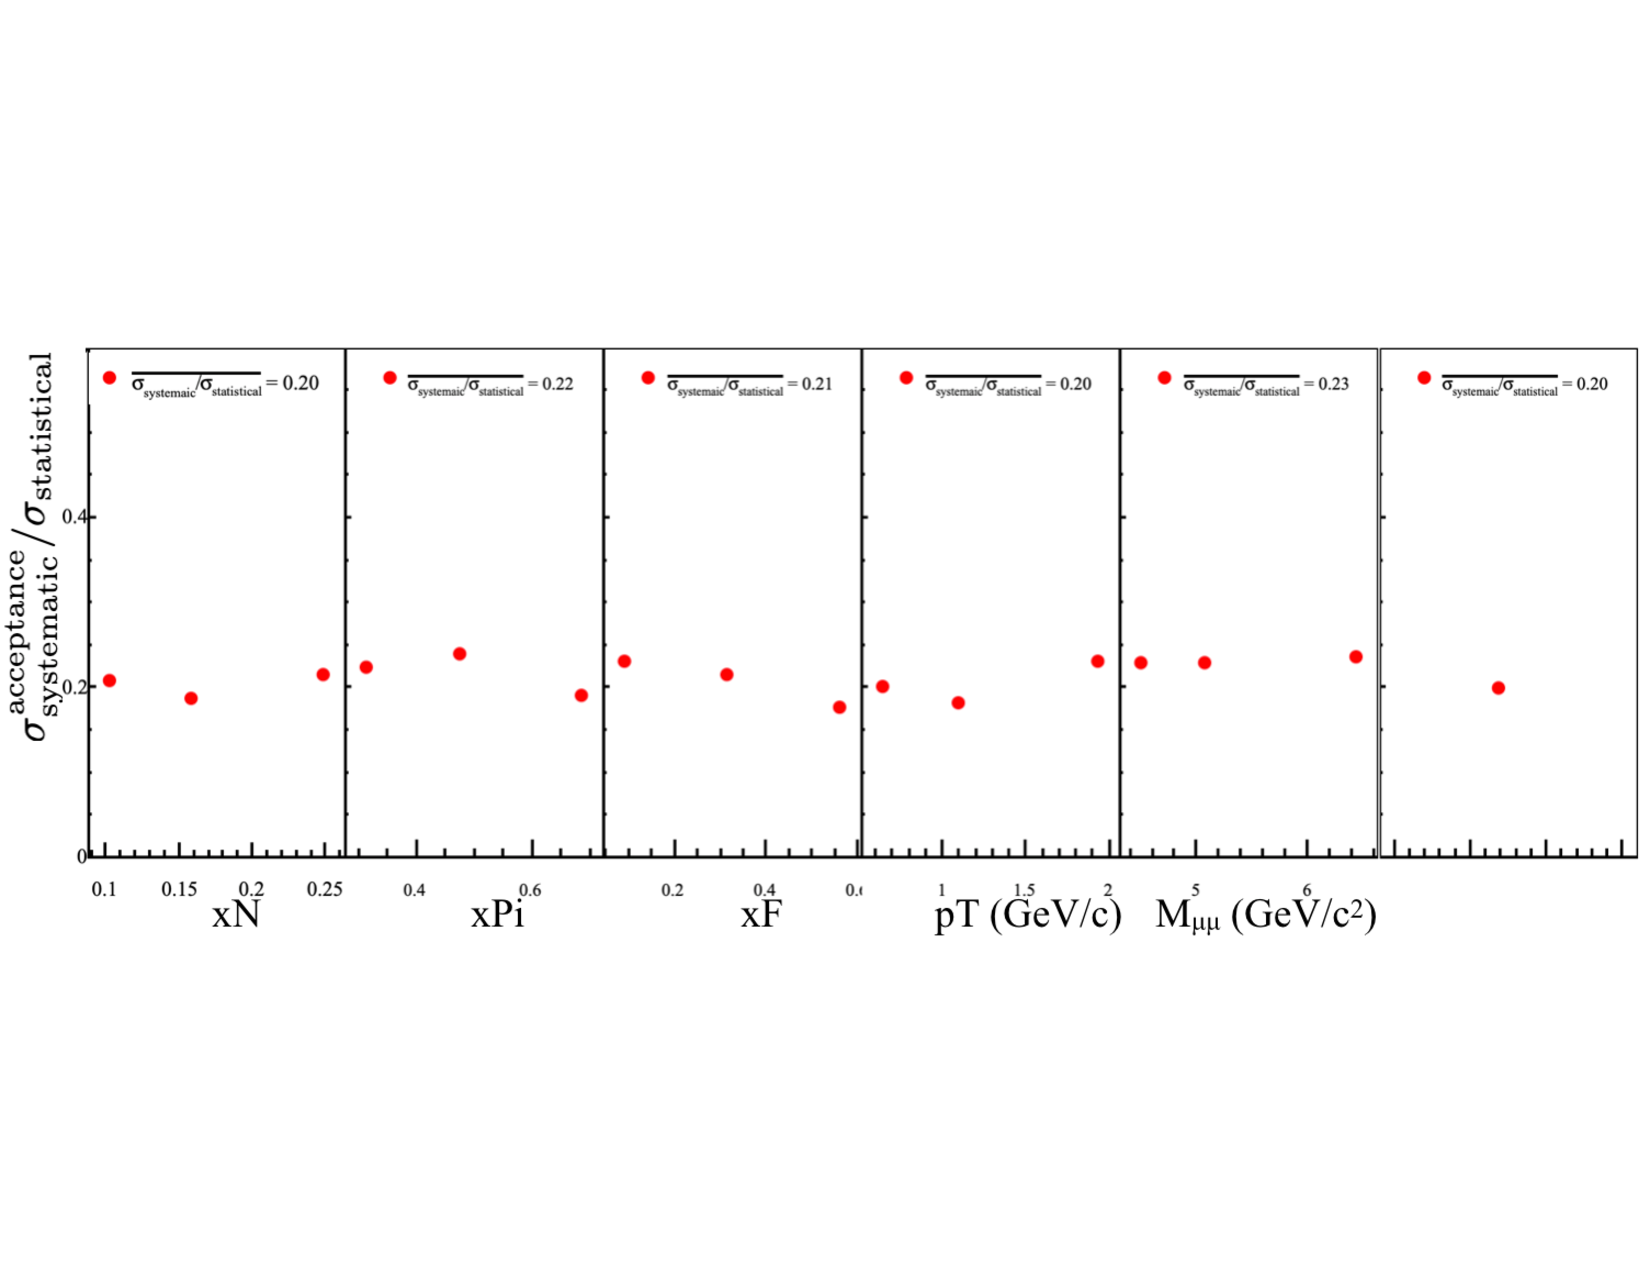
\includegraphics[width=\textwidth, trim=0cm 5cm 0cm 5cm,
      clip]{accSysStat}
    \caption{Systematic uncertainty due to acceptance effects normalized to the
      statistical error.}
    \label{fig::accSysStat}
  \end{center}
\end{figure}

\subsubsection{Further False Asymmetry Effects}
Although the list of systematic effects specifically studied is quite exhaustive
there is always the potential for other systematic effects not considered.
Studies of the changes in time from additional false asymmetries were performed
in an attempt to take into account all other systematic effects.  All false
asymmetries considered must be constructed in such a way that the physical
process of interest cancels out.  A false asymmetry could therefore only be
non-zero from acceptance effects, luminosity or some other reason not
considered.  The additional false asymmetries are constructed in a way that
luminosity effects cancel out and acceptance effects are approximately constant.
With these assumptions, the pull values from Eq.~\ref{eq::pull} are expected to
be distributed as a standard Gaussian distribution.  Any deviation from a
standard Gaussian is conservatively taken as a systematic effect from some
unknown cause.  The additional studied false asymmetries are summarized in the
following enumerated list.

\begin{enumerate}
  \label{tab::additionalFA}

\item A false asymmetry similar to Eq.~\ref{equ::falseAcc} but with the upstream
  left and right counts flipped defined as
  
  \begin{equation}
    \label{equ::additionalfalseAsym}
    A_{lr, F1} = \frac{1}{|S_T|}
    \frac{
      \sqrt[4]{
        N_{1,l}^\uparrow N_{1,r}^\downarrow N_{2,l}^\uparrow N_{2,r}^\downarrow
      }
      - \sqrt[4]{ N_{1,r}^\uparrow N_{1,l}^\downarrow
        N_{2,r}^\uparrow N_{2, l}^\downarrow }
      }{
      \sqrt[4]{
        N_{1,l}^\uparrow N_{1,r}^\downarrow
        N_{2,l}^\uparrow N_{2, r}^\downarrow
      } + \sqrt[4]{ N_{1,r}^\uparrow N_{1,l}^\downarrow
        N_{2,r}^\uparrow N_{2, l}^\downarrow
      }
    }.
  \end{equation}
  This false asymmetry can be thought of as measuring the normalized counts on
  the Jura side minus the Saleve side.  The period weighted average results of
  this false asymmetry are shown in Fig.~\ref{fig::fa2TargJuraSaleve}.  As
  Fig.~\ref{fig::fa2TargJuraSaleve} shows, the asymmetry is systematically less
  than zero by more than a standard deviation resulting from acceptance effects.
  The uncorrelated pull distributions from this false asymmetry are shown in
  Fig.~\ref{fig::fa2TargJSPulls} along with the corresponding Gaussian fit
  results.  Due to the fact that there are less entries in these pull
  distributions the Gaussian fit results are not necessarily that good.  In an
  attempt to correct for this and to take into account the fit errors, a
  weighted average of the mean and standard deviation are made, as in
  Eq.~\ref{equ::wAvg}, using weights as the inverse fit variances.  The
  resulting systematic error is again determined as in
  Eq.~\ref{equ::sysErrorPull} using the weighted mean and weighted standard
  deviation.

  \begin{figure}[h!t]
    \centering 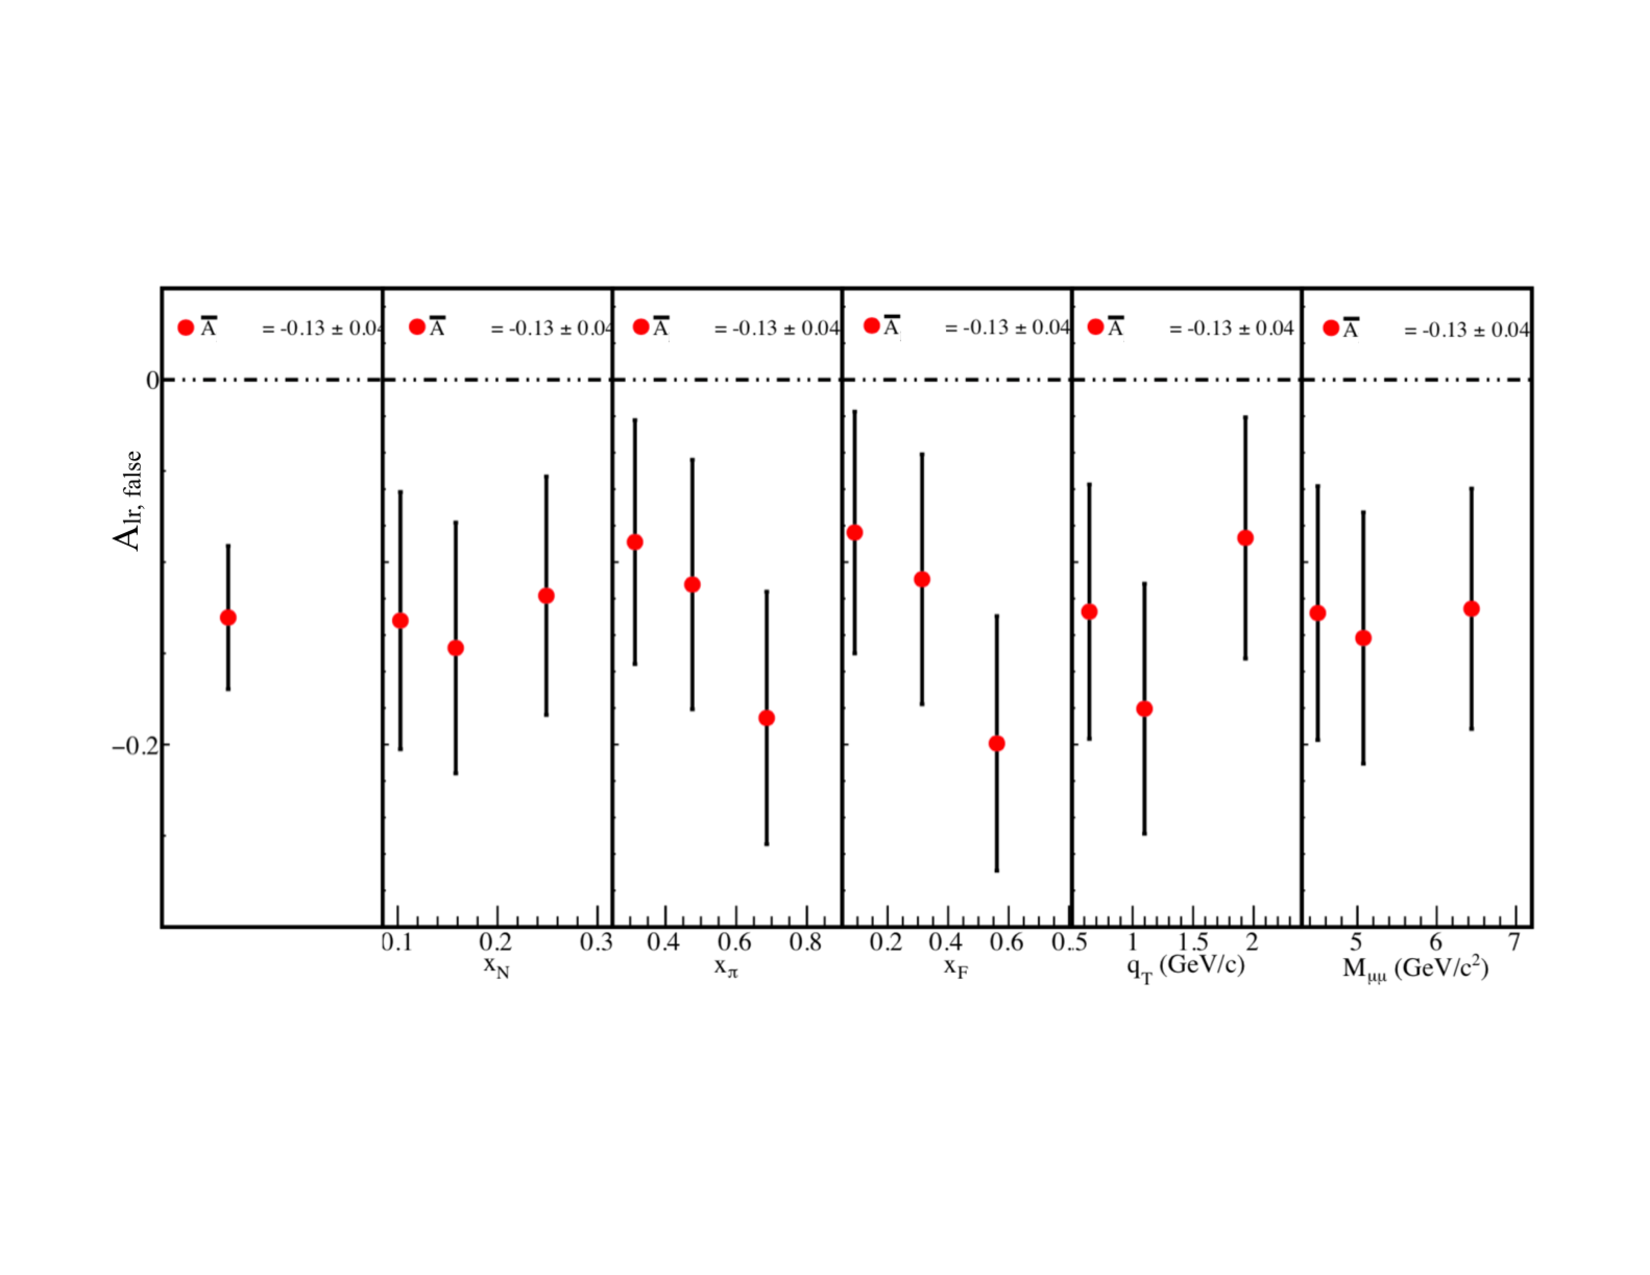
\includegraphics[width=0.9\textwidth, trim=1.5cm 4.5cm 1.5cm
      4.5cm, clip]{fa2TargJuraSaleve}
    \caption{Two-target geometric mean false asymmetry.  This is non-zero due to
      acceptance effects}
    \label{fig::fa2TargJuraSaleve}
  \end{figure}
  
  \begin{figure}[h!t]
    \centering 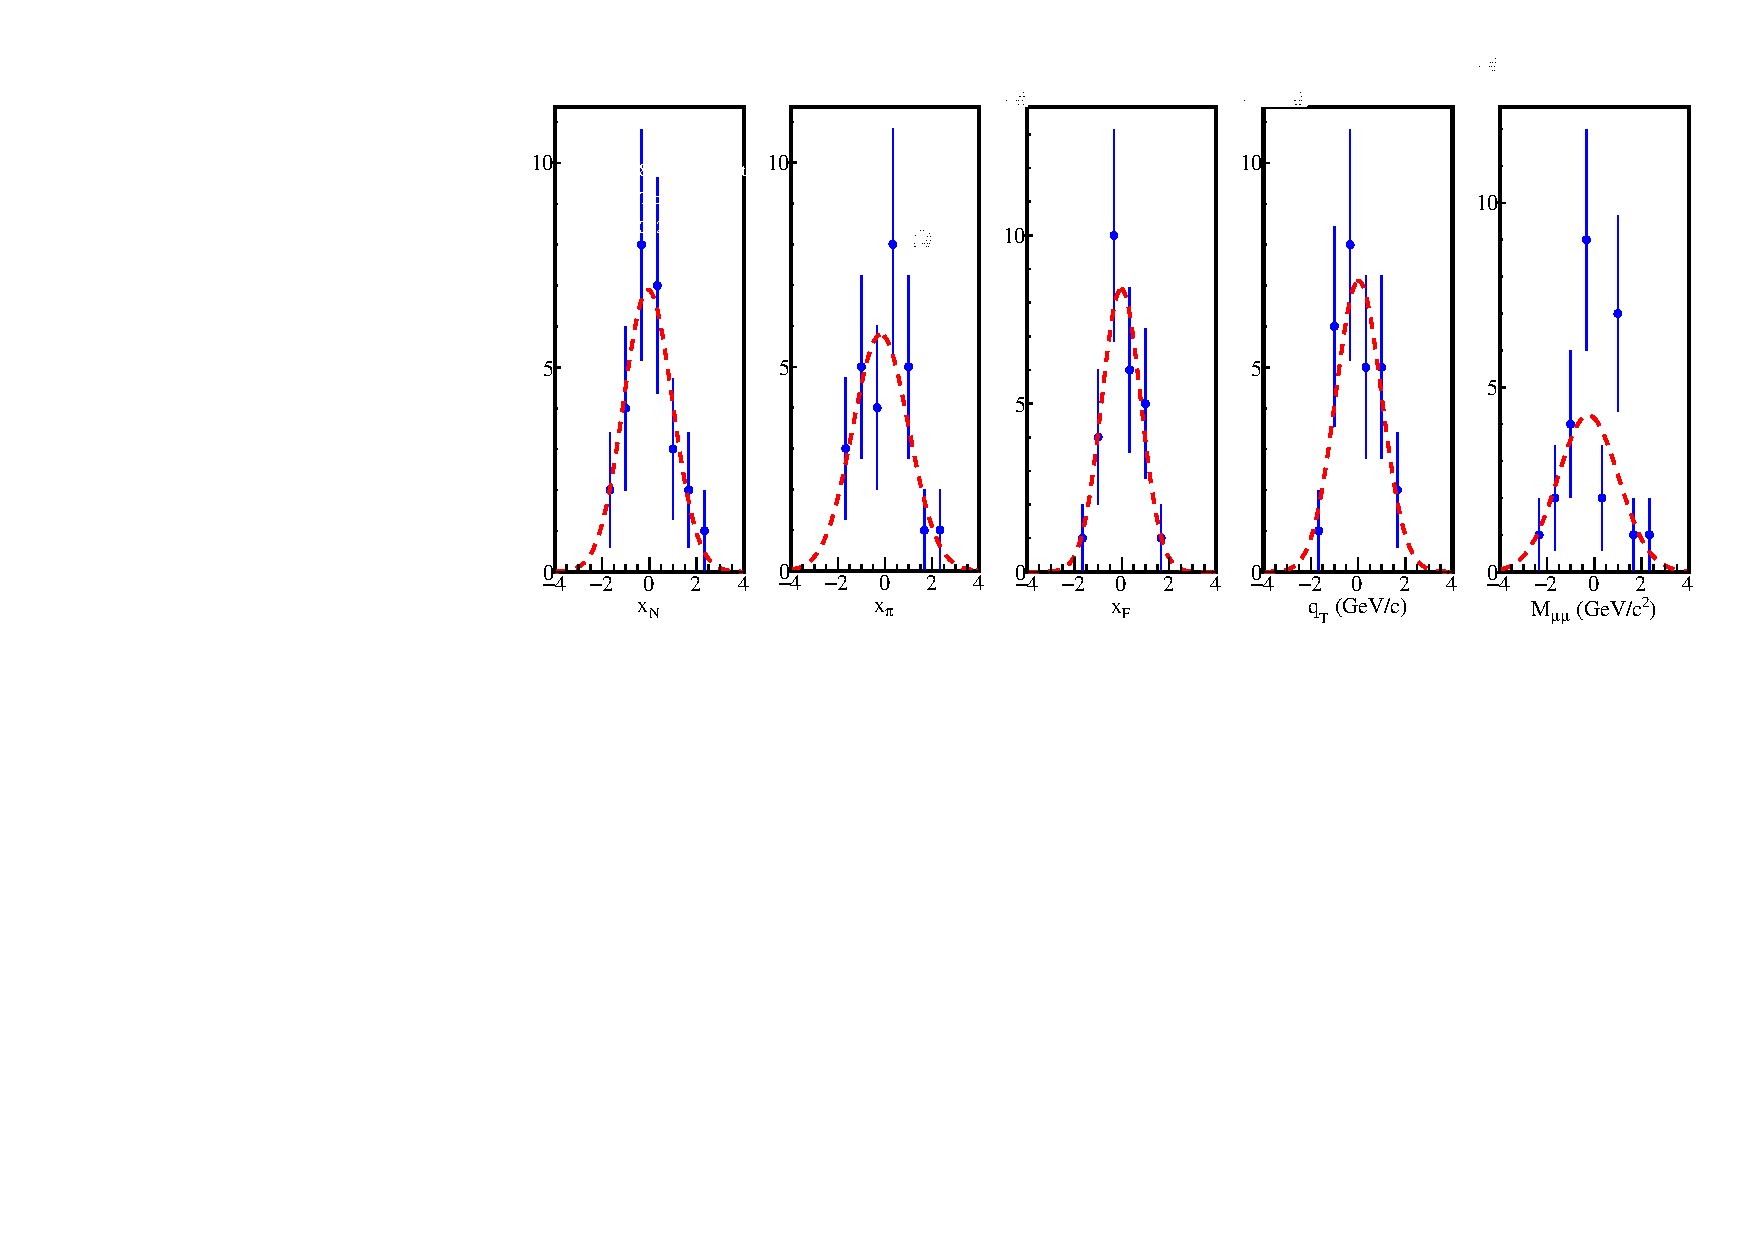
\includegraphics[width=0.9\textwidth, trim=1.5cm 2.5cm 1.5cm
      2.5cm, clip]{fa2TargJSPulls}
    \caption{Uncorrelated pulls of the two-target geometric mean false asymmetry
      and Gaussian fit results}
    \label{fig::fa2TargJSPulls}
  \end{figure}

\item A false asymmetries using only the information from the upstream or the
  downstream target defined as

  \begin{equation}
    \label{equ::falseANgeomean}
    A_{lr, F2} =
    \frac{1}{|S_T|}
    \frac{\sqrt{N_l^\uparrow N_r^\downarrow}
      - \sqrt{N_r^\uparrow N_l^\downarrow}
    }{
      \sqrt{N_l^\uparrow N_r^\downarrow}
      + \sqrt{N_r^\uparrow N_l^\downarrow}
    }.
  \end{equation}
  This false asymmetry can also be thought of as measuring the normalized counts
  on the Jura side minus the Saleve side but for each target individually.  Both
  this false asymmetry and the previous false asymmetry,
  Eq.~\ref{equ::additionalfalseAsym}, can be written as
  \begin{equation}
    A_{lr,F1/2} =
    \frac{1}{|S_T|}
    \frac{\alpha - 1}{\alpha + 1},
  \end{equation}
  where $\alpha$ will be an acceptance ratio of Jura/Saleve.  As the Jura/Saleve
  acceptance ratio is expected to be the same for the upstream and downstream
  targets, any difference between the two false asymmetries must be due to other
  reasons.  A by-period comparison between the upstream and downstream target is
  shown in Fig.~\ref{fig::alphaAsymPeriod} and as can be seen there are
  difference by-period between the upstream and downstream asymmetries.  A
  combined pull distribution is made using the information from both upstream
  and downstream asymmetries and is shown in Fig.~\ref{fig::alphaAsymPull}.  As
  with the previous false asymmetry, lack of data leads to the same problems
  with fit and therefore the same weighting method is used to determine a
  systematic error.

  \begin{figure}[h!t]
    \centering 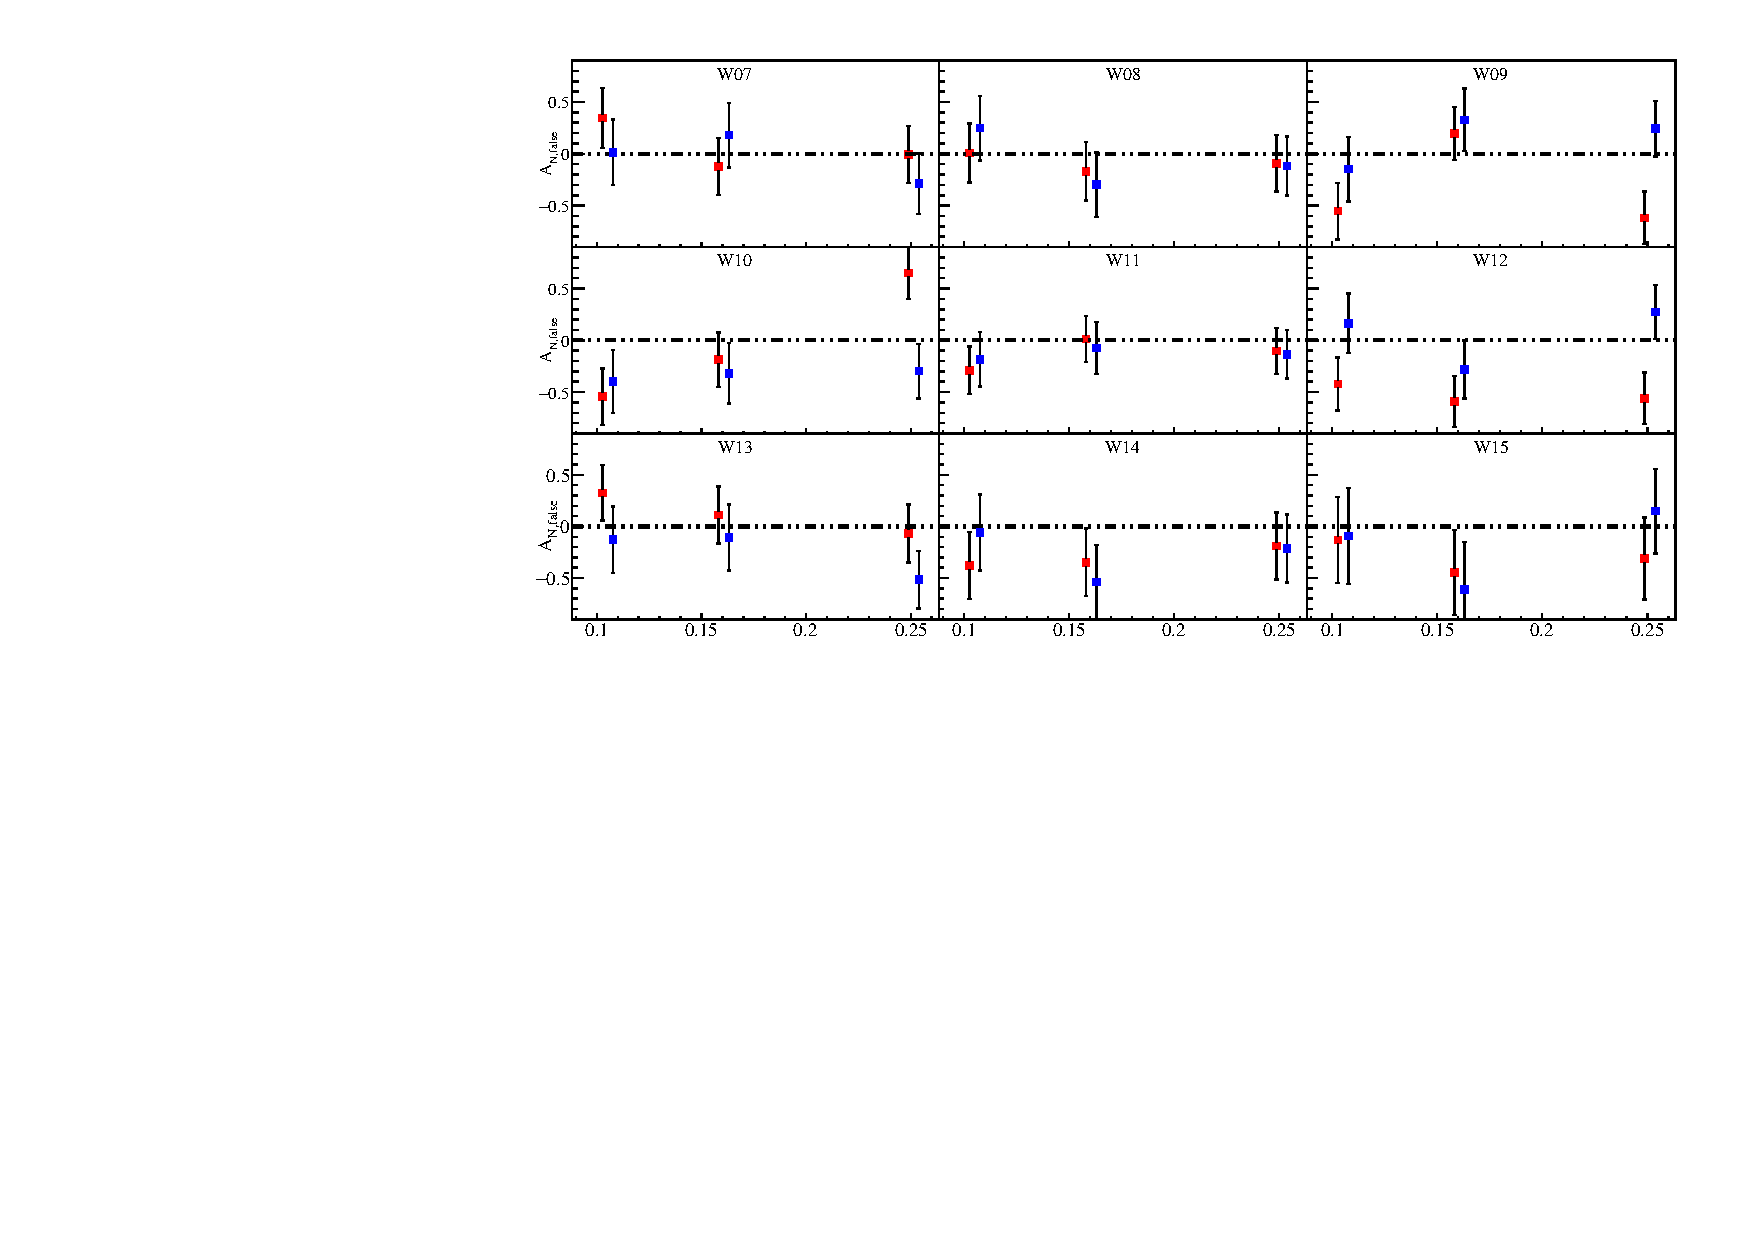
\includegraphics[width=\textwidth, trim=2cm 4cm 2cm 4cm,
      clip]{alphaAsymPeriod}
    \caption{One target false asymmetries for the upstream target (red) and the
      downstream target (blue), as a function of x$_{\mathrm{N}}$.  Each graph
      is from a different period in time.}
    \label{fig::alphaAsymPeriod}
  \end{figure}

  \begin{figure}[h!t]
    \centering
    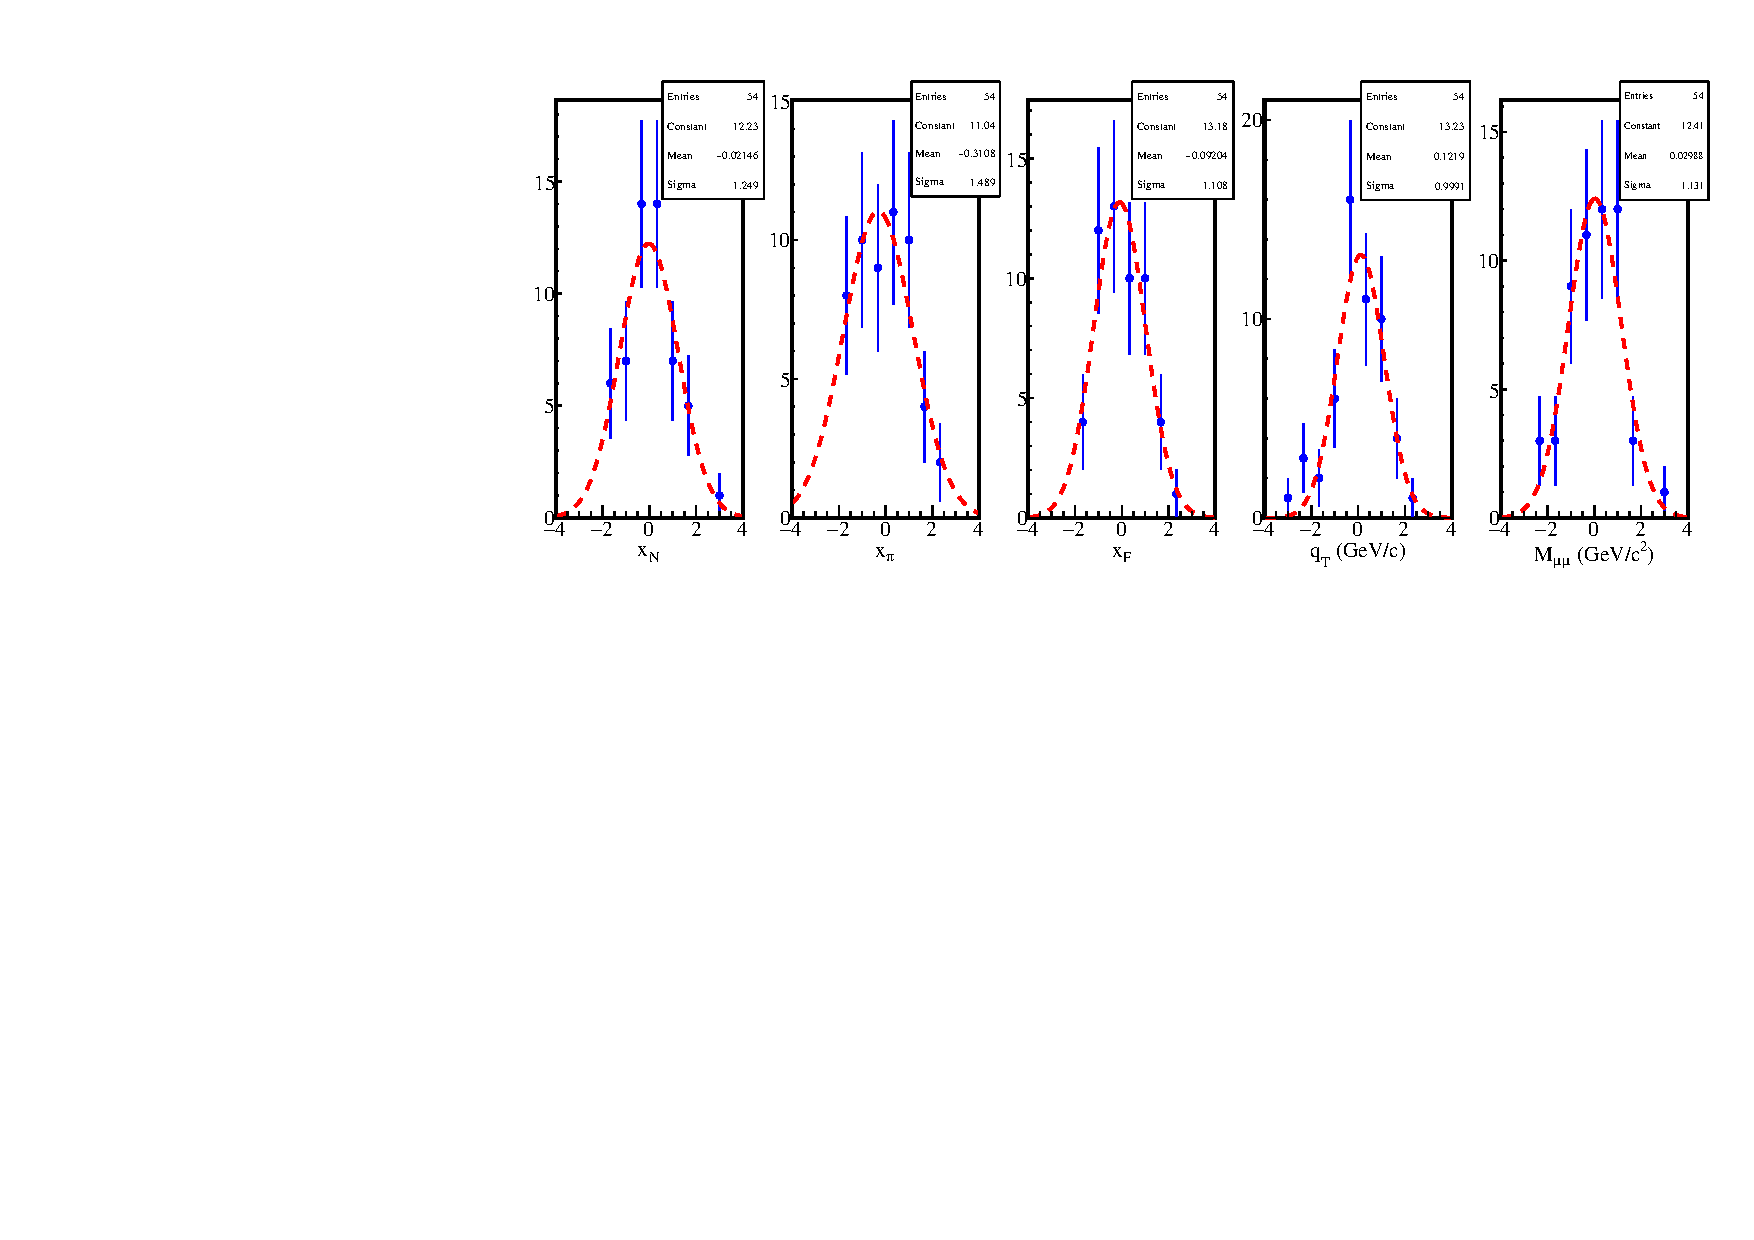
\includegraphics[width=\textwidth]{alphaAsymPull}
    \caption{Pull values from one-target geometric mean false asymmetries.  Both
      upstream and downstream values are used to make this pull}
    \label{fig::alphaAsymPull}
  \end{figure}

\item Finally the same false asymmetry used to determine the acceptance
  fluctuations, Eq.~\ref{equ::falseAcc}, is also checked for compatibility and a
  systematic error is determined in the same way as the previous false
  asymmetries.  The pulls are shown in Fig.~\ref{fig::fa2TargPulls} along with
  the corresponding fit parameters and errors.

  \begin{figure}[h!t]
    \centering 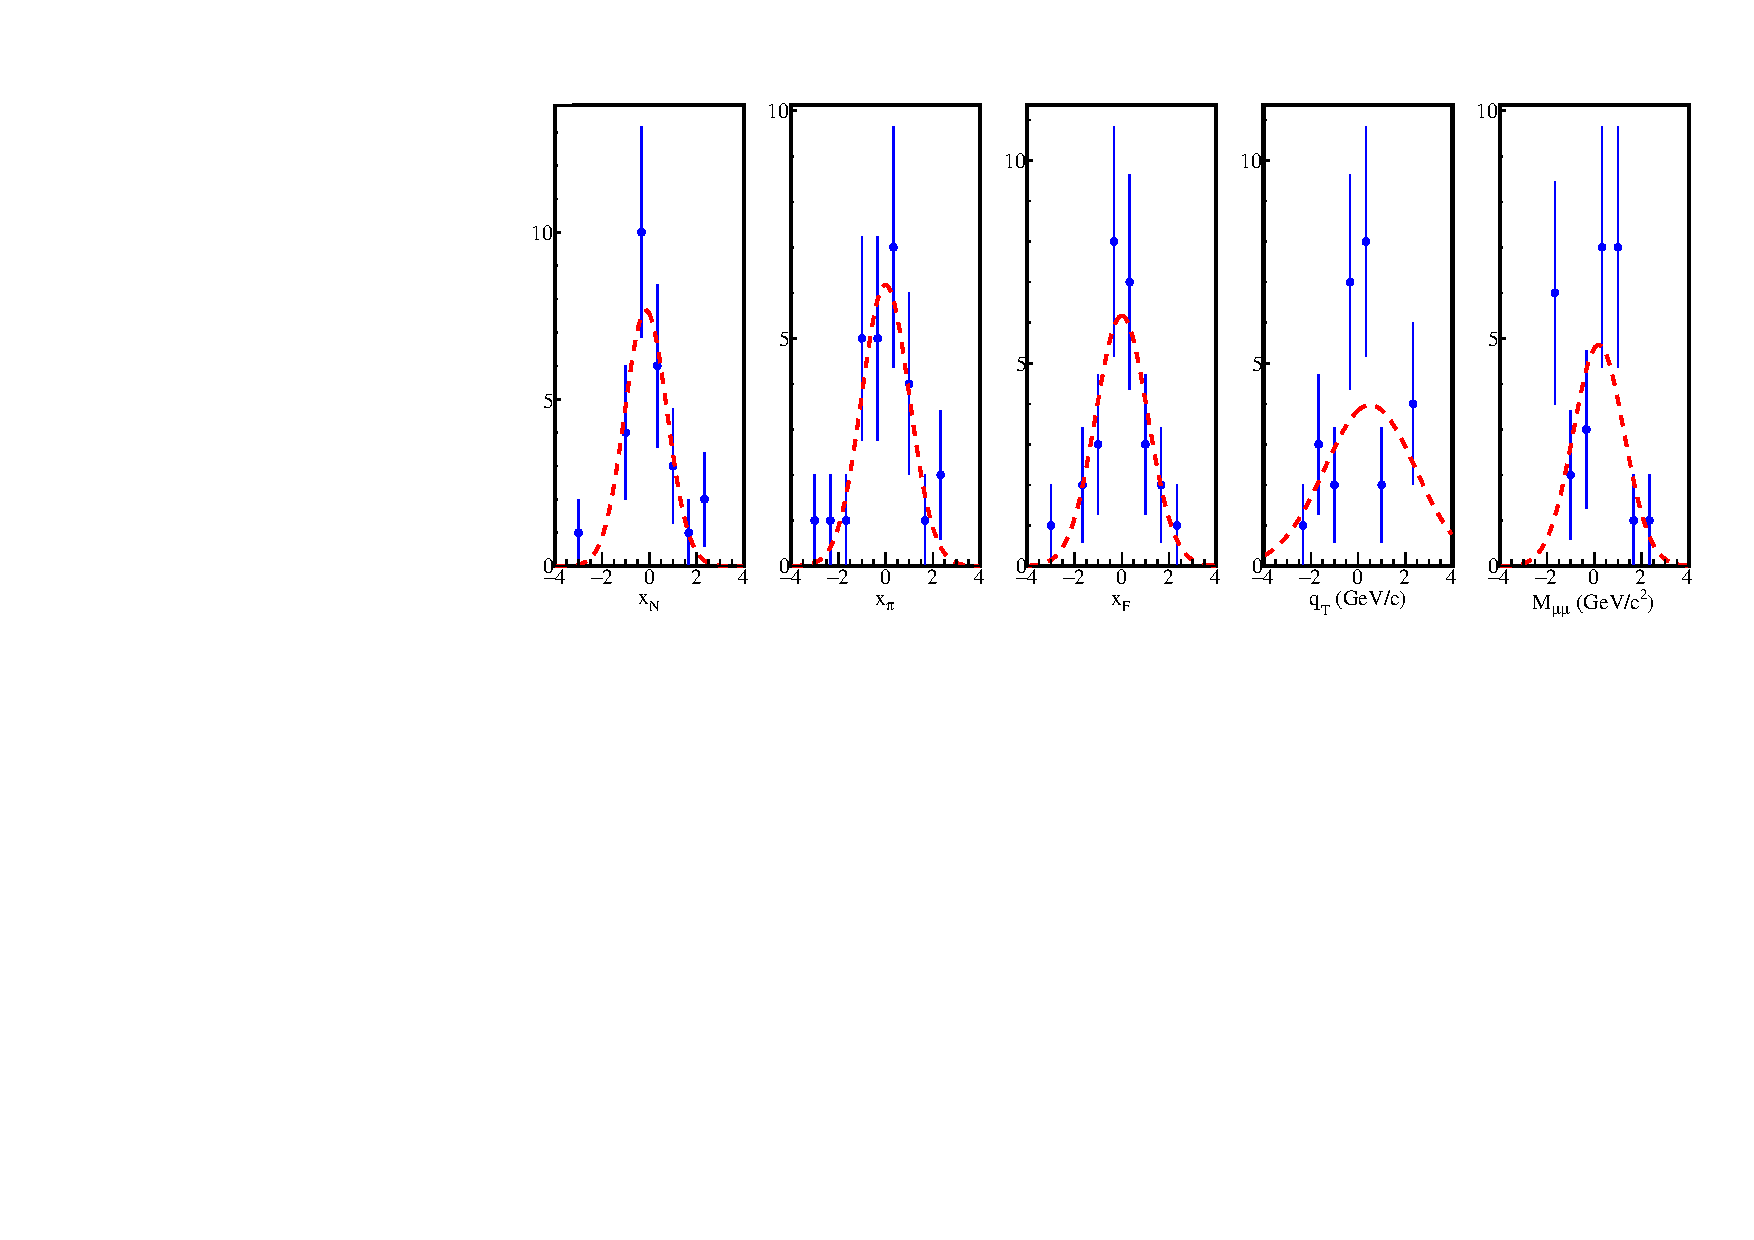
\includegraphics[width=\textwidth, trim=2.5cm 6cm 2.5cm 6cm,
      clip]{fa2TargPulls}
    \caption{Pull distribution for a nearly acceptance free two-target false
      geometric mean asymmetry}
    \label{fig::fa2TargPulls}
  \end{figure}
  
\end{enumerate}

A summary of the systematic error from each false asymmetry is shown in
Table.~\ref{tab::faSys}

\begin{table}[h!t]
  \centering
  \begin{tabular}{|c|c|}
    \hline Systematic error& \multirow{2}{9em}{$\langle
      \sigma_{\mathrm{systematic}}/\sigma_{\mathrm{statistical}}
      \rangle$}\\ & \\ \hline
    
    Two target Jura-Saleve& 0.26\\ \hline

    Combined one target& 0.5\\ \hline

    Two target acceptance estimation& 0.29\\ \hline
    
  \end{tabular}
  \caption{Summary of systematic error impacts from false asymmetries.  The
    maximum systematic error is chosen as the systematic error.}
  \label{tab::faSys}
\end{table}

\subsubsection{Total Systematics}
The total systematic uncertainty is determined by adding all non-zero systematic
effects in quadrature as

\begin{equation}
  \Big \langle \frac{
    \sigma_{\mathrm{systematic}}}{\sigma_{\mathrm{statistical}}} \Big \rangle =
  \sqrt{ \sum_i^{\mathrm{all \; systematic}} \Big \langle
    \frac{\sigma^2_{\mathrm{systematic, i}}}{\sigma^2_{\mathrm{statistical}}}
    \Big \rangle } \;,
\end{equation}
where all the systematic effects considered are summarized in
Table.~\ref{tab::sysError}.  For reference the integrated left-right asymmetry
is $\langle A_{lr} \rangle = 0.030$ and the integrated statistical error is
$\langle \sigma_{\mathrm{statistical}} \rangle$ = 0.039.

\begin{table}[h!t]
  \centering
  \begin{tabular}{|c|c|c|}
    \hline
    \multirow{2}{*}{Systematic Uncertainty}&
    \multirow{2}{*}{
      $\langle \sigma_{\mathrm{systematic}}/\sigma_{\mathrm{statistical}}
      \rangle$} &
    \multirow{2}{*}{$\langle \sigma_{\mathrm{systematic}} \rangle$}\\
    & & \\ \hline \hline

    Period compatibility& 0.0 & 0.0\\ \hline

    Left-Right migration& 0.09 & 0.004\\ \hline

    Target Polarization& 0.05& 0.003\\ \hline

    Dilution Factor& 0.05 & 0.003\\ \hline

    Acceptance fluctuation& 0.2 & 0.008\\ \hline

    False asymmetry& 0.5 & 0.020\\ \hline \hline
    \textbf{Total}& \textbf{0.55} & \textbf{0.022}\\\hline
    
  \end{tabular}
  \caption{Summary of systematic uncertainty impacts to the integrated
    asymmetry}
  \label{tab::sysError}
\end{table}

\subsection{Results} \label{sec::lr_results}
The left-right asymmetry is extracted per period, corrected for the target
polarization and ultimately combined as a weighed average, Eq.~\ref{equ::wAvg},
to get an overall result as in Sec~\ref{sec::doubleratio_results}.

The results for the geometric mean are shown in Fig.~\ref{fig::ANgeom} and the
results for the two-target geometric mean are shown in
Fig.~\ref{fig::AN4TargGeom}.  The numerical values for the two-target geometric
mean systematic uncertainty are summarized in Table~\ref{tab::sysError}.  To
verify the results in this section are correct, an independent cross-check was
performed by a member from the University of Turin and no discrepancies were
found.  The results of the cross-check are provided in
Appendix~\ref{app::xcheckAlr}.

\begin{figure}[h!t]
  \begin{center}
    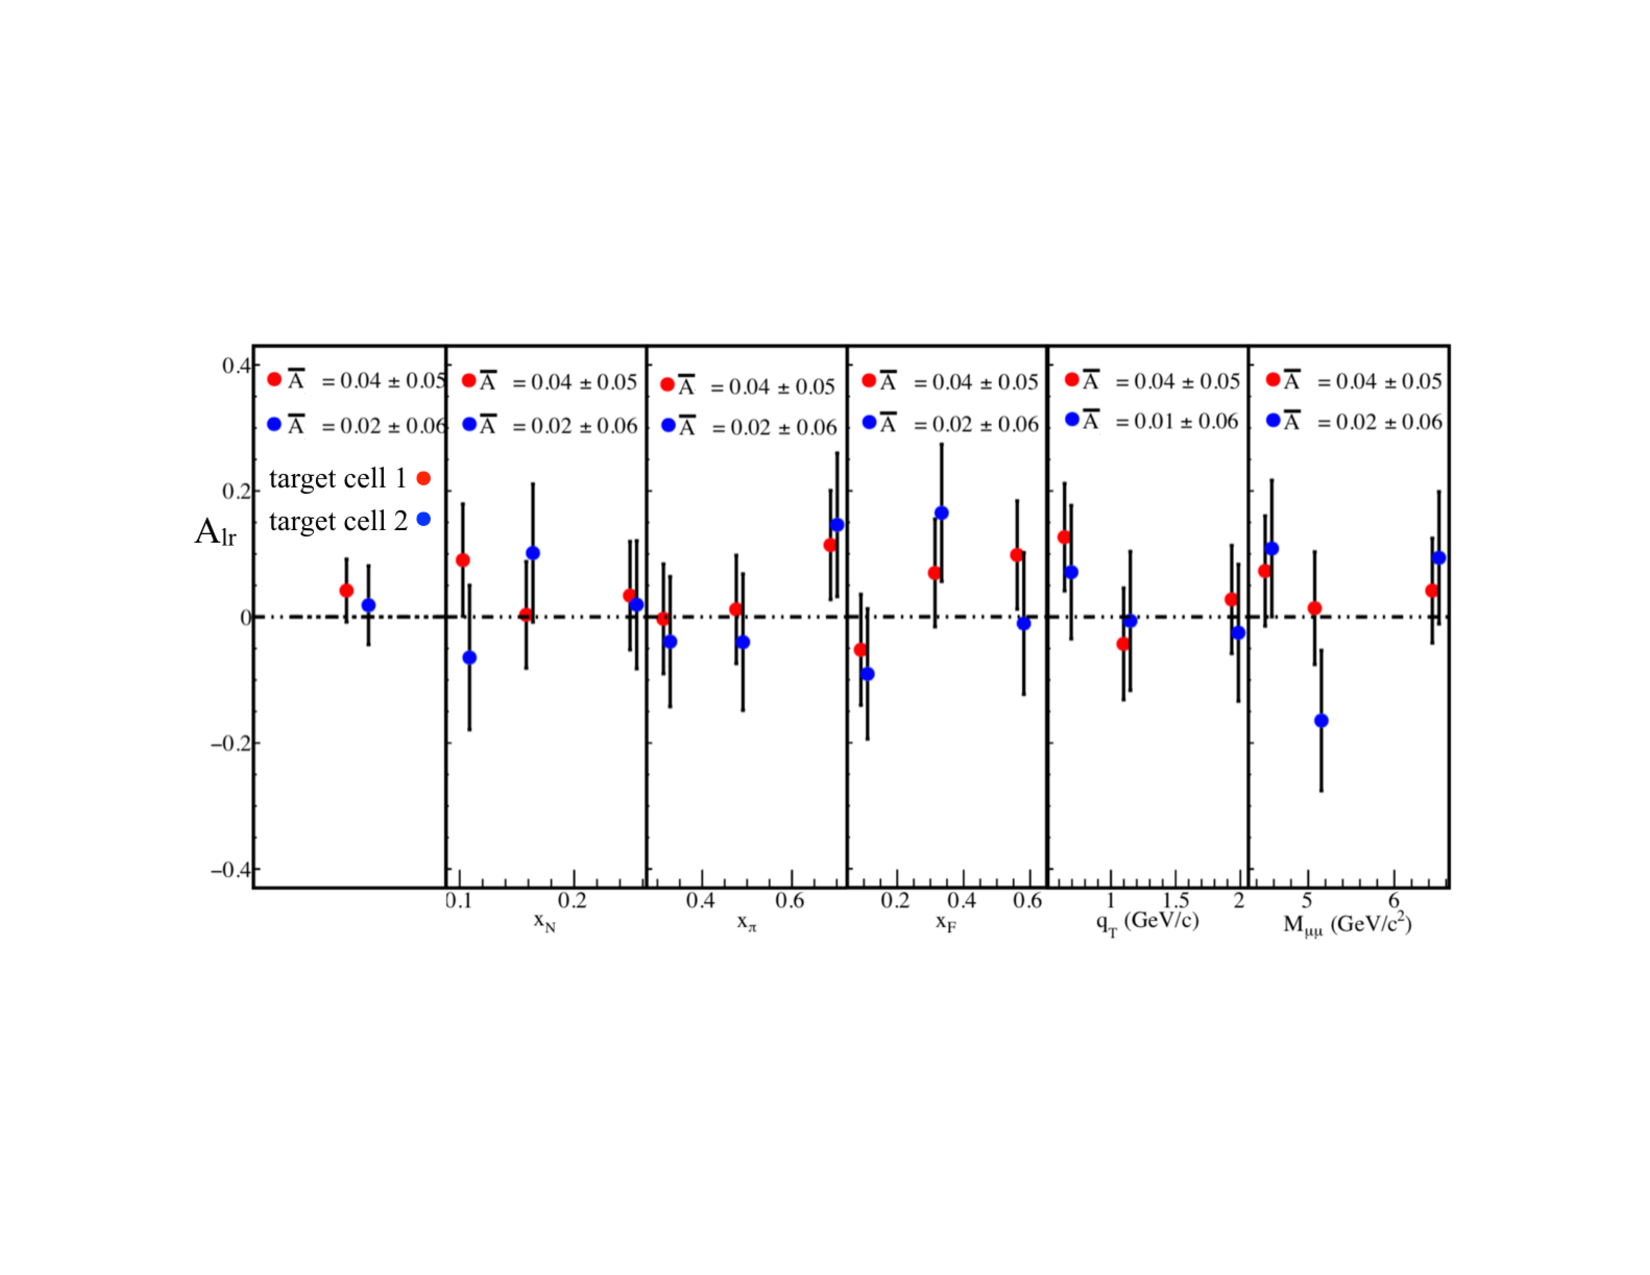
\includegraphics[width=\textwidth, trim=1cm 5.5cm 1cm 5.5cm,
      clip]{ANgeom}
    \caption{$A_{lr}$ determined from the geometric mean method for the upstream
      target cell (red) and the downstream target cell (blue) for all kinematic
      binnings}
    \label{fig::ANgeom}
  \end{center}
\end{figure}

\begin{figure}[h!t]
  \begin{center}
    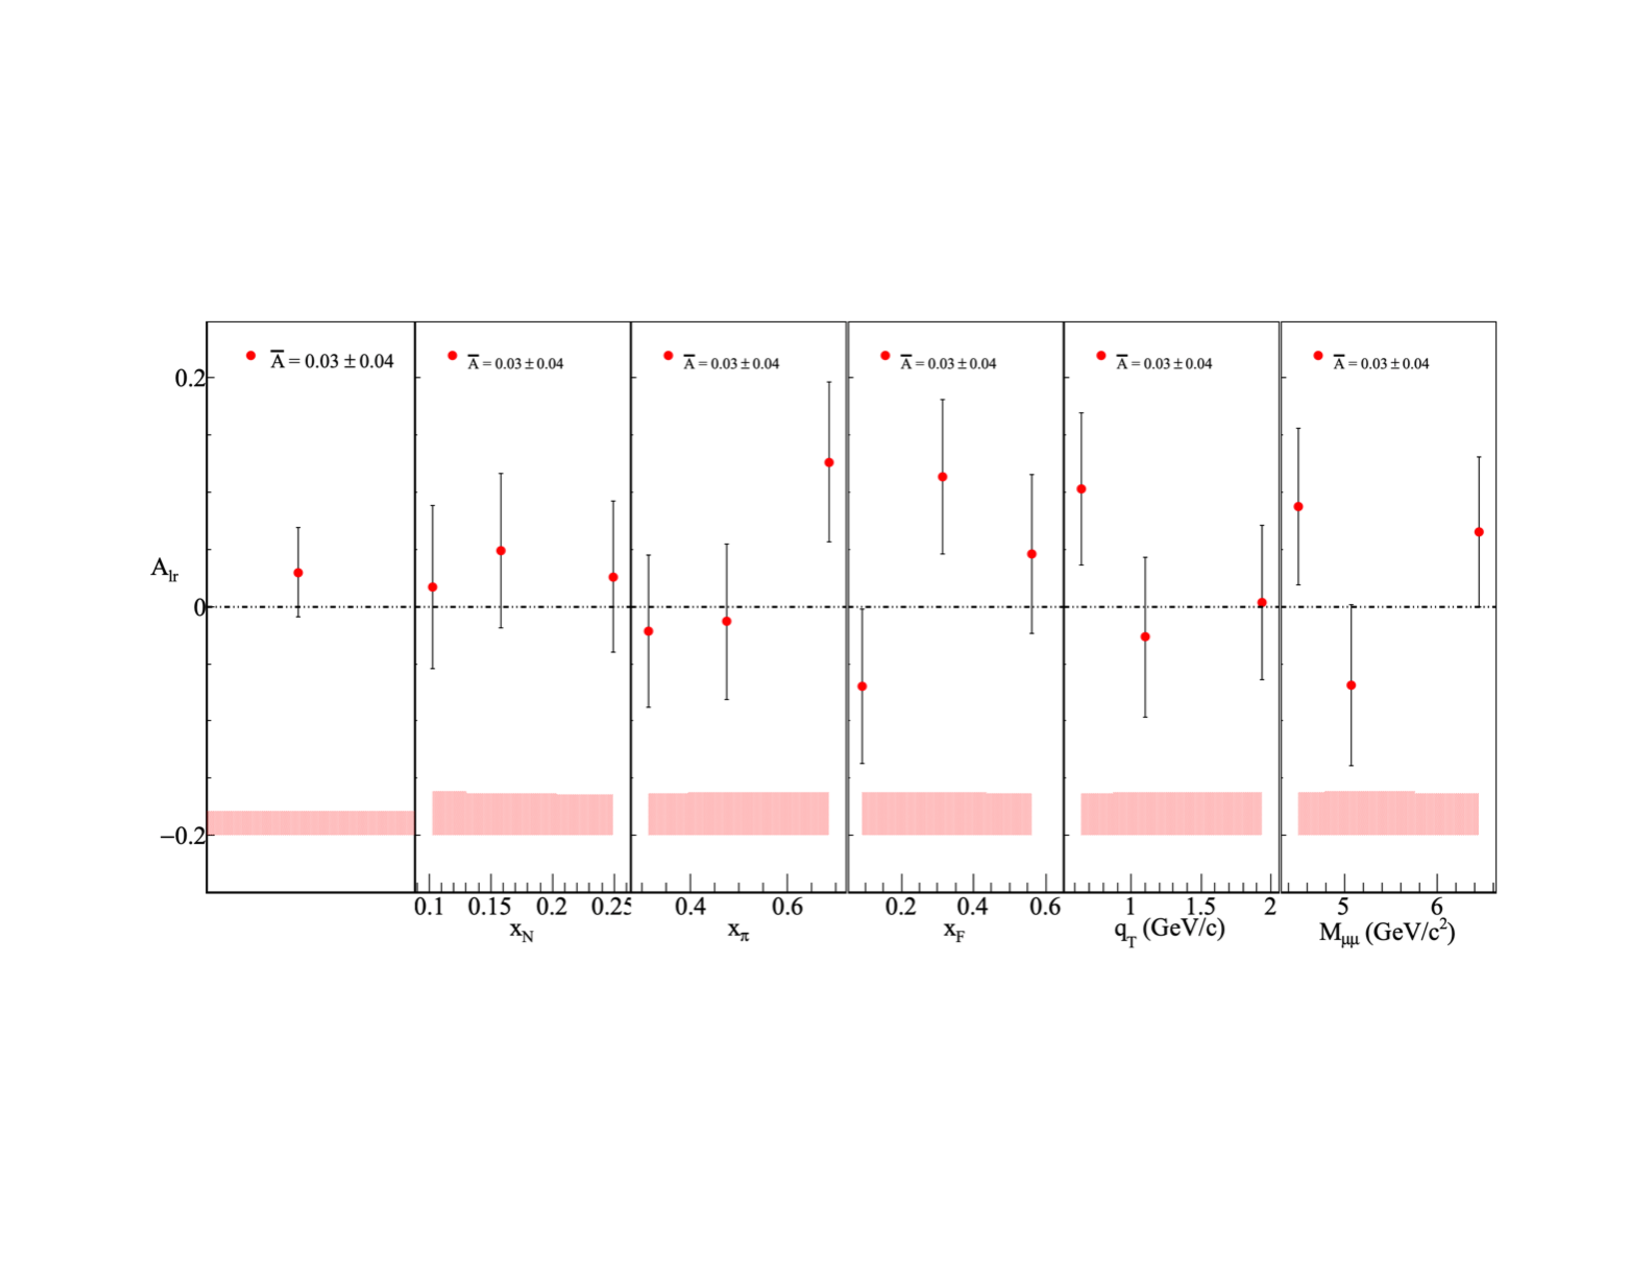
\includegraphics[width=\textwidth, trim=2cm 5cm 2cm 5cm,
      clip]{AN4TargGeom}
    \caption{$A_{lr}$ determined by the two-target geometric mean method
      for all kinematic binnings}
    \label{fig::AN4TargGeom}
  \end{center}
\end{figure}

It was shown in Sec~\ref{sec::lr_theory} that the left-right asymmetry is
related to the Sivers amplitude as

\begin{equation}
  \label{equ::all_an_convert}
  A_{lr} = \frac{2A^{\sin(\phi_S)}}{\pi} = \frac{2A_N}{\pi},
\end{equation}

\noindent
where $A_N$ is the analyzing power.  The Sivers amplitude was measured to be
approximately 1 sigma above zero from the unbinned maximum likelihood method,
Fig.~\ref{fig::DY_Siv_signFlip}, the double ratio method,
Fig.~\ref{fig::dr_final_results}, and the left-right asymmetry.  Adjusting the
left-right asymmetry, as in Eq.~\ref{equ::all_an_convert}, shows the amplitude
determined from the left-right asymmetry is statistically consistent with the
Sivers amplitude determined from the double ratio method,
Fig.~\ref{fig::AN_DR_comp}.  Therefore all methods to determine the Siver
amplitude in this chapter are consistent with the sign flip hypothesis between
the Drell-Yan and SIDIS processes.  On the other hand, the statistical error
bars are too large to definitively conclude the sign flip assumption holds.
There are also no clear trends in the kinematic variable binning due to the
large statistical error bars.

It is interesting to note that Eq.~\ref{equ::all_an_convert} was derived with
the assumption that the leading order Drell-Yan cross-section,
Eq.~\ref{equ::DY_MostusefulXsect}, is sufficient.  It is not theoretically ruled
out however, that the left-right asymmetry results from higher order amplitudes
in addition to the Sivers amplitude.  As Fig.~\ref{fig::AN_DR_comp} shows, the
left-right asymmetry is slightly less significant about zero than the Sivers
amplitude determined from the double ratio method.  This could indicate the need
to include higher order terms in the Drell-Yan cross-section.

\begin{figure}[h!t]
  \centering 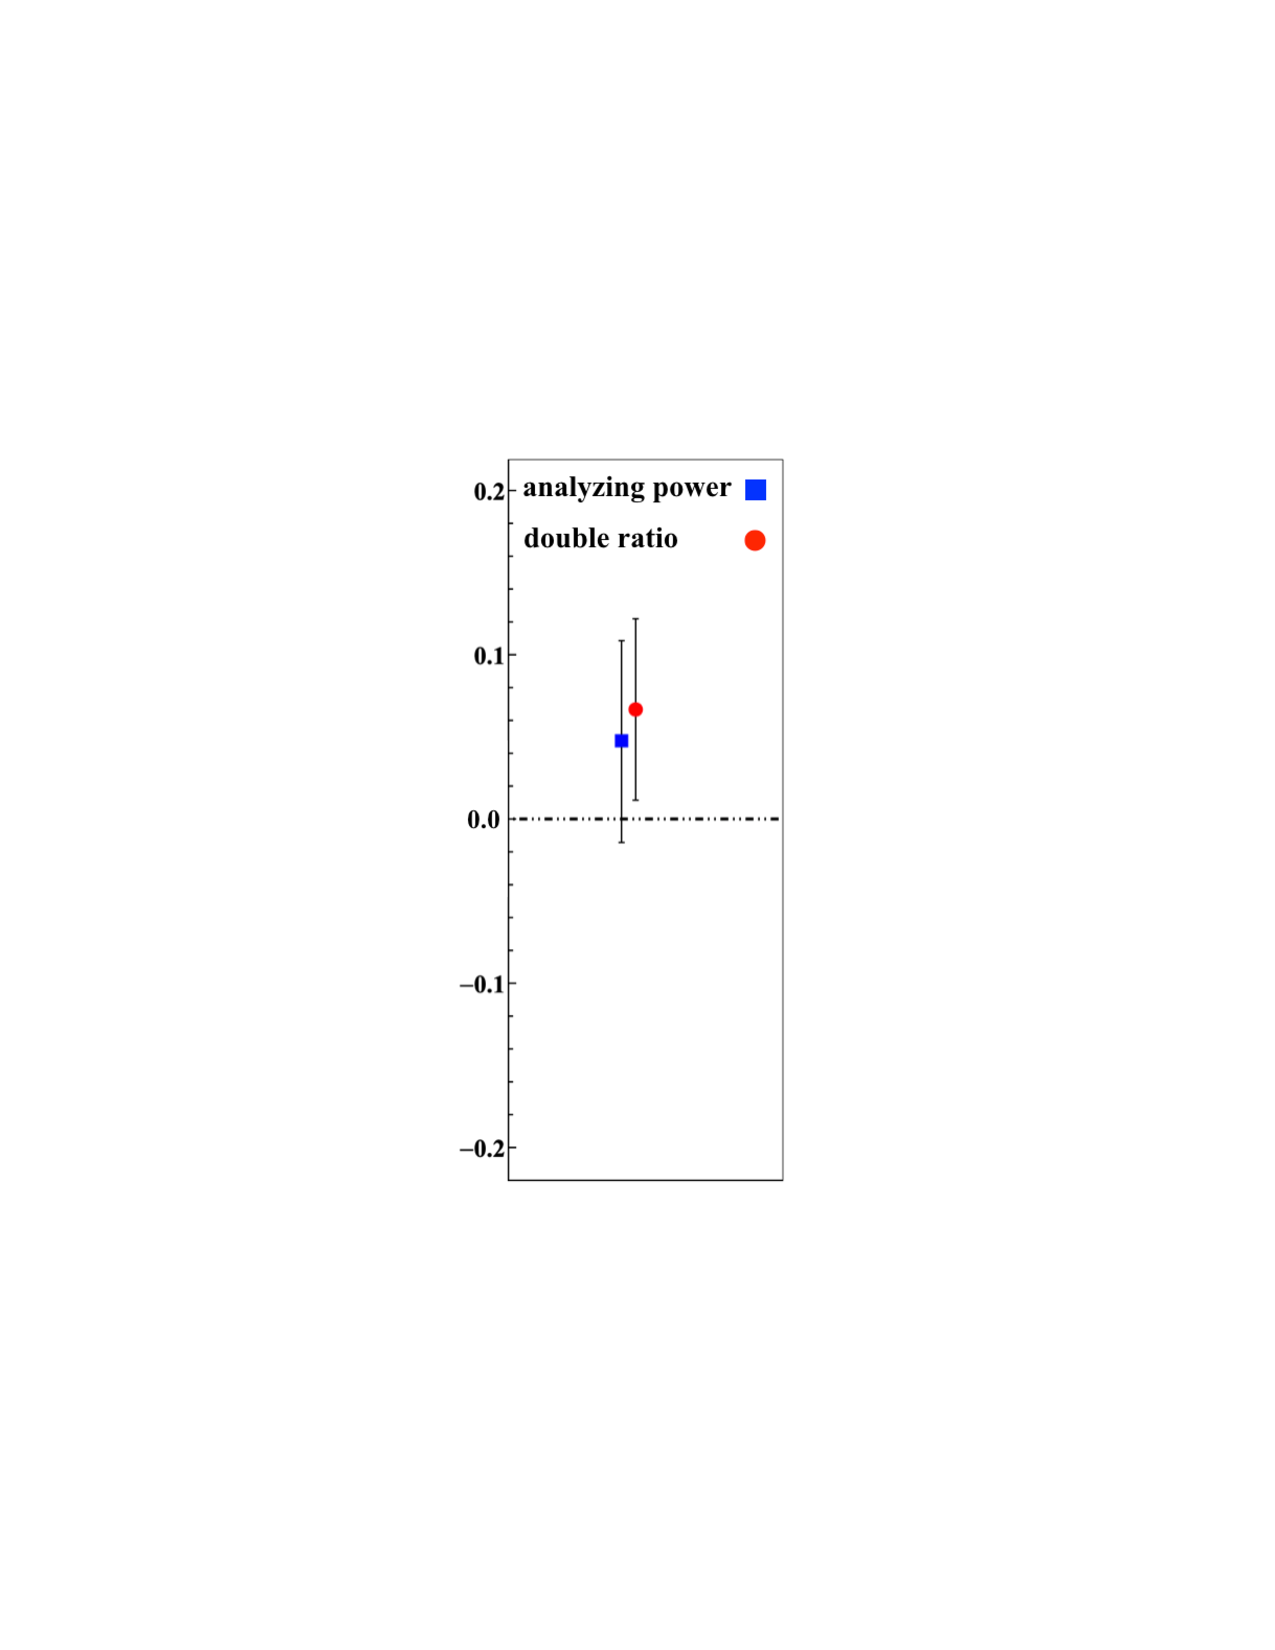
\includegraphics[width=0.2\textwidth, trim=7.5cm 7.5cm 7.5cm
    7.5cm, clip]{AN_DR_comp}
  \caption{The left-right asymmetry adjusted (analyzing power, blue) to be
    compared with Sivers amplitude determined from the double ratio method
    (red).}
  \label{fig::AN_DR_comp}
\end{figure}


%\begin{table}[h!t]
%  \centering
%  \label{tab::AN4TargGeom}
%  \caption{Two-target geometric mean numerical values and error bars for each
%    kinematic bin}
%  \begin{tabular}{ |c|c|c|c|c| }
%    \hline \textbf{Binning variable}& \textbf{Bin Range}&
%    \textbf{A}$_{\mathrm{\textbf{N}}}$&
%    \textbf{$\delta$}\textbf{A}$^{\mathrm{\textbf{stat}}}_{\mathrm{\textbf{N}}}$&
%    \textbf{$\delta$}\textbf{A}$^{\mathrm{\textbf{sys}}}_{\mathrm{\textbf{N}}}$
%    \\ \hline \hline
%
%    $\langle$ {\xn} $\rangle$& & & & \\
%  \end{tabular}
%\end{table}
